\documentclass[aspectratio=169]{beamer}
\usepackage[utf8]{inputenc}

\setbeamersize{text margin left=3mm,text margin right=3mm} 

\usetheme{Oxygen}
\usepackage{hyperref}
%\usepackage{movie15}
\usepackage{textpos}
\usepackage{fancybox}
\usepackage{colortbl}
\usepackage{rotating}
\usepackage{pgfplots}
% \usepackage{subfigure}
%\usepackage{subcaption}
\usepackage{multicol}
\usepackage{multirow}
\usepackage{amsmath,amssymb,amsfonts,amsbsy,dsfont}
\usepackage{mathrsfs}
\usepackage{amsthm}
\usepackage{bm}
\usepackage{array}
%\usepackage[caption=false]{subfig}
\usepackage{arydshln}
\usepackage{breakcites}
\usepackage{booktabs}
\usepackage{tabularx}
\usepackage{makecell}
\usepackage{amsmath}
\usepackage{tikz}
\usepackage{pgf-pie}
\usepackage{epsfig,epic,eepic,threeparttable,amscd,here,lscape,tabularx,graphicx }
\usepackage{booktabs}
\usepackage{tabu,array}
\usepackage{overpic}
\usepackage{microtype}

\usepackage{subcaption}
\usetikzlibrary{decorations.pathreplacing}

\definecolor{GII}{RGB}{255,255,107}
\definecolor{GI}{RGB}{72,197,72}
\definecolor{GIII}{RGB}{214, 36, 47}

\providecommand{\ppunto}[2]{\langle#1, #2 \rangle}% producto punto
\providecommand{\promed}[1]{{\mathbb{E}}\left\lbrace #1\right\rbrace}% operador de promedio
\providecommand{\promeddd}[2]{\mathbb{E}_{#1}\!\left\{#2\right\}}% op{\tiny }erador de promedio
\providecommand{\promedd}[2]{\mathds{E}_{#1}\left\{#2\right\}}% operador de promedio
\providecommand{\cov}[2]{{\fam=7 cov}\{#1, #2\}}% operador de covarianza
\providecommand{\gaus}[2]{{\fam=6 N}(#1 #2)} % FDP Gauss
% Kronecker delta function
\providecommand{\Kronecker}[2]{\delta_{K}( #1 , #2 )}
% cardinality
\providecommand{\Cardinality}[1]{| #1 |}

\let\oldcite\cite % store the original \cite command
\renewcommand{\cite}[1]{{\tiny\oldcite{#1}}}

\usepackage{bm}

\usepackage{etoolbox}

\DeclareUnicodeCharacter{2212}{-}

\newcommand{\ve}[1]{\bm {#1}}
\newcommand{\mat}[1]{\bm {#1}}
\usepackage[nopar]{lipsum} 

\newif\ifcomment
\newcommand{\Com}{\par\footnotesize\itshape\commenttrue}

\newenvironment{Itemize}
 {%
  \edef\Itemizecurrent{\the\font}%
  \itemize
  \preto{\item}{\ifcomment\par\Itemizecurrent\fi}%
 }{%
  \enditemize
 }


\title[]{Regularized Gaussian Functional Connectivity Network with Post-Hoc Interpretation for Improved EEG-based Motor Imagery-BCI Classification}
\vskip -0.7cm
\author{\normalsize{Daniel Guillermo Garc\'ia Murillo}\\ \scriptsize{dggarciam@unal.edu.co
}}
\institute{\includegraphics[width=0.15\textwidth]{../Tesis_document/Figures/EscudoUN2016.jpg}\\\scriptsize{
Universidad Nacional de Colombia \\ Signal Processing and Recognition Group - SPRG
\\
Advisor: Andrés Marino Álvarez-Meza, Ph.D.\\
Co-advisor: César Germán Castellanos-Domíguez, Ph.D.\\
\vspace{-0.3cm}
}}

% \date[]{\scriptsize{Signal Processing and Recognition Group - SPRG\\
% Department of Electrical, Electronic and Computer Engineering\\
% Universidad Nacional de Colombia - Sede Manizales\\
% 2024}}
\date[]{\scriptsize{\today}}



\setbeamercovered{dynamic}
\setbeamertemplate{navigation symbols}{}

\begin{document}

{\setbeamertemplate{headline}{}
\setbeamertemplate{footline}{}
\begin{frame}{}
\vspace{-0.7cm}
    \titlepage 
\end{frame}
}


\newif\iflattersubsect

% \AtBeginSection[] {
%     \begin{frame}
%     \frametitle{Outline} %
%     \tableofcontents[currentsection, sections={1-6}]  
%     \end{frame}
%     \lattersubsectfalse
% }

% \AtBeginSection[] {
%     \begin{frame}
%     \frametitle{Outline I} %
%     \tableofcontents[currentsection, sections={1-6}]  
%     \end{frame}
%     \only<7-9>{
%         \begin{frame}
%         \frametitle{Outline II} %
%         \tableofcontents[currentsection, sections={7-9}]  
%         \end{frame}
%     }
%     \lattersubsectfalse
% }

\AtBeginSection[] {
    \ifnum\thesection<7
        \begin{frame}
        \frametitle{Outline I} %
        \tableofcontents[currentsection, sections={1-6}]  
        \end{frame}
    \else
        \begin{frame}
        \frametitle{Outline II} %
        \tableofcontents[currentsection, sections={7-9}]  
        \end{frame}
    \fi
    \lattersubsectfalse
}

\AtBeginSubsection[] {
    \ifnum\thesection<7
        \begin{frame}
        \frametitle{Outline I} %
        \tableofcontents[currentsubsection, sections={1-6}]  
        \end{frame}
    \else
        \begin{frame}
        \frametitle{Outline II} %
        \tableofcontents[currentsubsection, sections={7-9}]  
        \end{frame}
    \fi
    \lattersubsectfalse
}

\section[Motivation]{Motivation}

\begin{frame}{Brain computer interface (BCI)}
    \centering
    BCI provides people with external world communication by translating brain signals.~\cite{khan2020review}
    \begin{figure}[!ht]
        \centering
        \resizebox{0.8\linewidth}{!}{\includegraphics{figures/Motivation_BCI.png}}
        % \caption{Functional connectivity estimators classified based on direct or indirect, time or frequency domain and linear or nonlinear. The varying shades of orange represent different sensitivities to volume conduction.}
    \end{figure}

\end{frame}

\begin{frame}{Socioeconomic facts}
    \begin{columns}
        \column{0.6\textwidth}
        \begin{figure}
            \centering
            \resizebox{0.7\linewidth}{!}{\includegraphics{figures/pie_bci}}
            % \includegraphics[width=0.7\linewidth]{figures/BCI_applications.png}
            % \caption{Distribution of BCI Applications~\footnotemark[1].}
        \end{figure}
        \column{0.4\textwidth}
            \begin{itemize}
                \item Over 150 companies specializing in BCI as of 2019.
                \item BCI market valued at $228$ million in 2019, projected to reach $460$ million by 2029~\footnotemark[2].
            \end{itemize}
    \end{columns}
    \footnotetext[1]{\textbf{{Image}:} {Adapted from} \href{https://www.weforum.org/agenda/2024/06/the-brain-computer-interface-market-is-growing-but-what-are-the-risks/}{The World Economic Forum 2024}}
    \footnotetext[2]{\href{https://www.marketreportsworld.com/enquiry/request-sample/23789843}{Global Brain Computer Interface Market Research Report 2023}}
\end{frame}


\begin{frame}{Motor Imagery (MI)}
    \centering
    MI is a widely studied BCI paradigm that allows external motor communication~\cite{cattan2018recommendations}.
    \vspace{3em}
    \begin{columns}
        \column{0.5\textwidth}
        \centering
        \includegraphics[width=0.7\linewidth]{figures/Motor_imagery.png}
        \column{0.5\textwidth}
            \textbf{Applications:}
            \begin{itemize}
                \item Recovery of motor functionality \cite{bonci2021introductory}.
                \item Motor rehabilitation \cite{sitaram2017closed}.
                \item Virtual reality  \cite{cattan2018recommendations}.
                \item Gaming \cite{ahn2014review}.
                \item Skill acquisition \cite{casimo2017bci}.
            \end{itemize}
    \end{columns}
\end{frame}

\begin{frame}{Neuroimaging techniques}
    \begin{columns}
        \column{0.3\textwidth}
            \begin{itemize}
                \item MI involves fast-evolving cognitive processes \cite{varbu2022past}
                \item EEG and MEG have remarkable temporal precision \cite{alsharif2020neuromarketing}
                \item EEG is portabile and cost-effective \cite{janapati2023advances, hosseini2020review}
            \end{itemize}
        \column{0.7\textwidth}
            \begin{figure}[h!]
                \centering
                \resizebox{1\linewidth}{!}{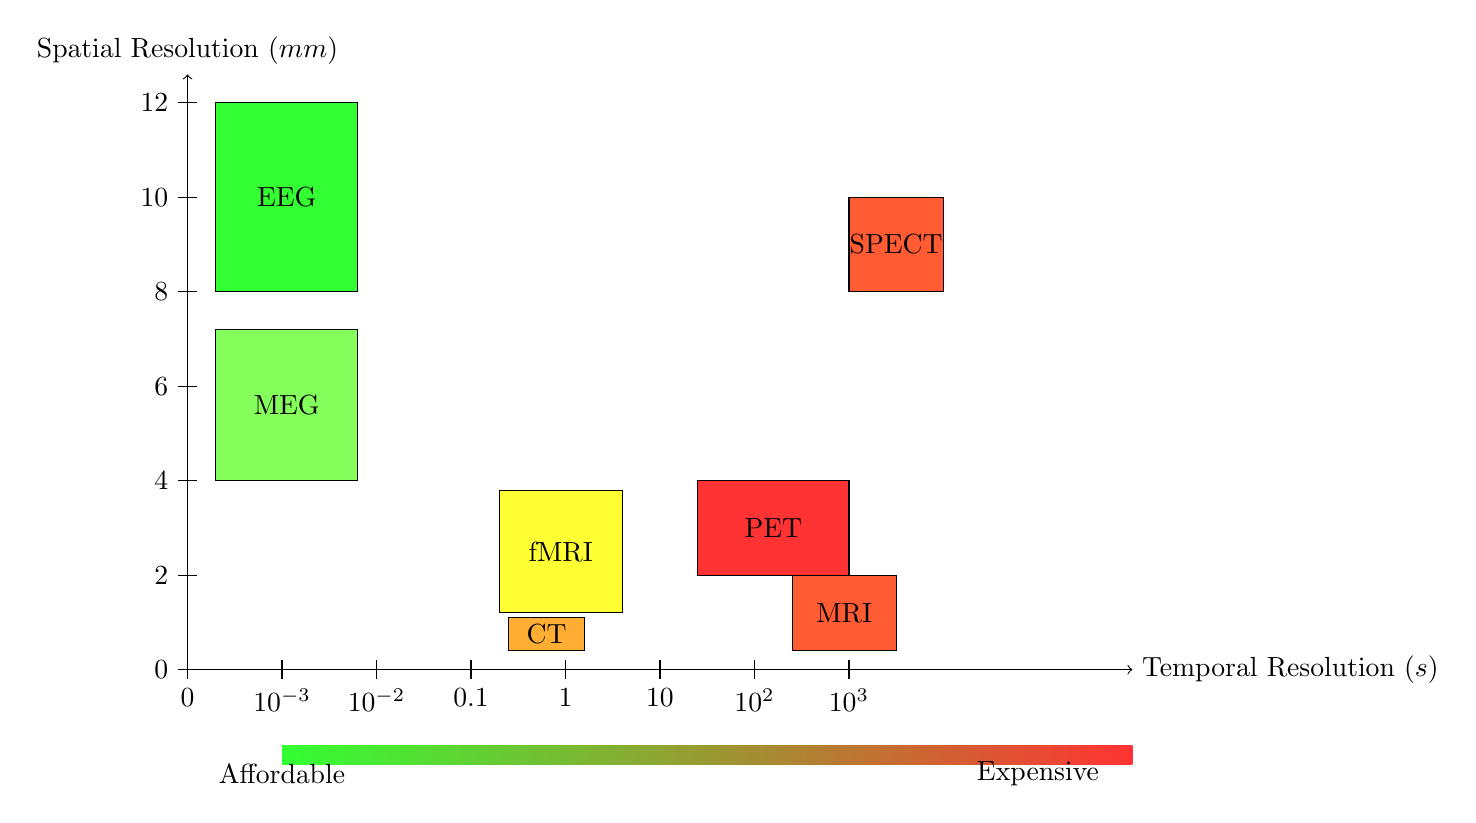
\begin{tikzpicture}[scale=1.2]

% Draw axes
% EEG 0.2
% MEG 0.4
% fMRI 0.8
% CT 0.6
% MRI 0.7
% PET 0.9
% SPECT 0.8

\definecolor{eegcolor}{HTML}{00FF00}
\definecolor{megcolor}{HTML}{66FF33}
\definecolor{fmricolor}{HTML}{FFFF00}
\definecolor{ctcolor}{HTML}{FF9900}
\definecolor{mricolor}{HTML}{FF3300}
\definecolor{petcolor}{HTML}{FF0000}
\definecolor{spectcolor}{HTML}{FF3300}
% X-axis labels
\draw[->] (0,0) -- (10,0) node[right] {Temporal Resolution $(s)$};
\draw (0,0.1) -- (0,-0.1) node[below] {$0$};
\draw (1,0.1) -- (1,-0.1) node[below] {$10^{-3}$};
\draw (2,0.1) -- (2,-0.1) node[below] {$10^{-2}$};
\draw (3,0.1) -- (3,-0.1) node[below] {$0.1$};
\draw (4,0.1) -- (4,-0.1) node[below] {$1$};
\draw (5,0.1) -- (5,-0.1) node[below] {$10$};
\draw (6,0.1) -- (6,-0.1) node[below] {$10^2$};
\draw (7,0.1) -- (7,-0.1) node[below] {$10^3$};

% Y-axis labels
\draw[->] (0,0) -- (0,6.3) node[above] {Spatial Resolution $(mm)$};
\draw (0.1,0) -- (-0.1,0) node[left] {$0$};
\draw (0.1,1) -- (-0.1,1) node[left] {$2$};
\draw (0.1,2) -- (-0.1,2) node[left] {$4$};
\draw (0.1,3) -- (-0.1,3) node[left] {$6$};
\draw (0.1,4) -- (-0.1,4) node[left] {$8$};
\draw (0.1,5) -- (-0.1,5) node[left] {$10$};
\draw (0.1,6) -- (-0.1,6) node[left] {$12$};

\fill[left color=eegcolor!80, right color=petcolor!80] (1,-1) rectangle ++(9,0.2);

\draw (9,-1.1) node[align=center] {Expensive};
\draw (1,-1.1) node[align=center] {Affordable};

% EEG (x,y)
\draw[fill=eegcolor!80] (0.3,4) rectangle (1.8,6) node[pos=.5] {EEG};

% MEG
\draw[fill=megcolor!80] (0.3,2) rectangle (1.8,3.6) node[pos=.5] {MEG};

% fMRI
\draw[fill=fmricolor!80] (3.3,0.6) rectangle (4.6,1.9) node[pos=.5] {fMRI};

% CT
\draw[fill=ctcolor!80] (3.4,0.2) rectangle (4.2,0.55) node[pos=.5] {CT};

% MRI
\draw[fill=mricolor!80] (6.4,0.2) rectangle (7.5,1) node[pos=.5] {MRI};

% PET
\draw[fill=petcolor!80] (5.4,1) rectangle (7,2) node[pos=.5] {PET};

% SPECT
\draw[fill=spectcolor!80] (7,4) rectangle (8,5) node[pos=.5] {SPECT};

\end{tikzpicture}}
                % \caption{Comparison of neuroimaging techniques: spatial and temporal resolutions, and relative costs}\label{fig:neuroimagig}
            \end{figure}
    \end{columns}
\end{frame}

\begin{frame}{Experimental setup for MI-based BCIs}
    \begin{columns}
        \column{0.6\textwidth}
            \begin{figure}[!ht]
                \centering
                \includegraphics[width=0.8\linewidth]{../Tesis_document/Figures/preliminaries/EEG-setup.png}
                % \caption{Experimental setup for MI-based BCIs. \textbf{{Source}
                %         :} {Adapted from} \cite{grigorev2021bci}}
            \end{figure}
        \column{0.4\textwidth}
            \begin{itemize}
                \item EEG headsets are equipped with $1$ to $256$ electrodes \cite{grigorev2021bci}.
                \item Visual cues are often used to guide MI tasks during EEG recordings \cite{hosseini2020review}.
            \end{itemize}
    \end{columns}
    \footnotetext[1]{\textbf{{Image}:} {Adapted from} \cite{grigorev2021bci}}
\end{frame}


\begin{frame}{Sensorimotor rhythms (SMRs)}
    \begin{columns}
        \column{0.4\textwidth}
            \begin{itemize}
                \item EEG signals contains multiple electrical variations (rhythms) \cite{barios2019synchronization}.
                \item Sensorimotor Rhythms (SMRs) occur in the brain's sensorimotor cortex \cite{altaheri2023deep}. 
                \item SMRs contain spectral-spatio-temporal patterns of MI tasks \cite{li2019motor}.
            \end{itemize}
        \column{0.6\textwidth}
            \begin{figure}[!ht]
                \centering
                \includegraphics[width=0.7\linewidth]{figures/SM_area.png}
            \end{figure}
    \end{columns}
    \footnotetext[1]{\textbf{{Image}:} {Adapted from} \cite{bookbiology20001}}
\end{frame} 


\begin{frame}{MI-EEG feature extraction}
    \begin{columns}
        \column{0.7\textwidth}
            \begin{figure}[!ht]
                \centering
                \includegraphics[width=0.7\linewidth,trim={0 0 0 10},clip]{figures/RAW_EEG.png}
                % \caption{Raw EEG signal representation}
            \end{figure}
        \column{0.3\textwidth}
            \begin{itemize}
                \item High number of channels and sampling rate \cite{chevallier2024largest}.
                \item Huge number of data points \cite{singh2021comprehensive}.
                \item Feature extraction strategies are required to reduce dimentionality \cite{ai2019feature}.
            \end{itemize}
    \end{columns}
    \centering
    
\end{frame}

\begin{frame}{Single channel feature extraction}
    \begin{columns}
        \column{0.4\textwidth}
            \begin{itemize}
                \item Capture rhythms on specific EEG channels \cite{samuel2017towards}.
                \item Time domain: statistical \cite{hamedi2014neural}, Hjorth \cite{yilmaz2018quasi}, etc.
                \item Spetral domain: Power spectral density \cite{oikonomou2017comparison}, Welch's periodigram \cite{roy2022comparative}, spectral entropy \cite{sarraf2017eeg}, etc.
            \end{itemize}
        \column{0.6\textwidth}
            \begin{figure}[!ht]
                \centering
                \includegraphics[width=0.6\linewidth,trim={0 110 40 40},clip]{figures/Cxsbj1gaussacc86.85-eps-converted-to.pdf}
                % \caption{Brain area activation when performing motor imagery tasks}
            \end{figure}
    \end{columns}
    \vspace{3em}
    \centering
    Executing or imagining motor tasks activates multiple brain areas,\\patterns that single-channel features fail to capture \cite{chiarion2023connectivity}.
\end{frame}


\begin{frame}{Multi channel feature extraction}
    \begin{columns}
        \column{0.5\textwidth}
            \begin{figure}[!ht]
                \centering
                \includegraphics[width=1\linewidth]{figures/connectivities.png}
                % \caption{Three  types of brain connectivity: structural, effective, and functional, each describing interactions between brain regions \cite{ismail2020graph}.}
            \end{figure}
        \column{0.5\textwidth}
            \begin{itemize}
                \item Structural connectivity (SC) focuses on physical connections, fails to capture short-living events \cite{thiebaut2020brain}
                \item Effective connectivity (EC) describes direct connections and requires deep cognitive process understanding to select the best causal model \cite{chiarion2023connectivity}.
                \item Functional connectivity (FC) can describe directed or non-directed connectives usually via statistical correlation \cite{cao2022brain}
            \end{itemize}
    \end{columns}
    \vspace{3em}
    \centering
    FC's simplicity, low computational demands, and lack of rigid assumptions\\ make it ideal for MI-BCI applications \cite{he2019electrophysiological}.
\end{frame}

\begin{frame}{Signal Processing and Recognition Group - SPRG}
    \centering
    The SPRG has been working on the design of ML and DL models to improve\\ the performance and explainability of EEG-based MI-BCIs \cite{collazos2023posthoc}.
    \centering
    \includegraphics[width=0.7\linewidth]{figures/bcisoft.jpeg}
\end{frame}

\section{Problem statement}

\begin{frame}{Problem statement}
    \begin{figure}[!ht]
        \centering
        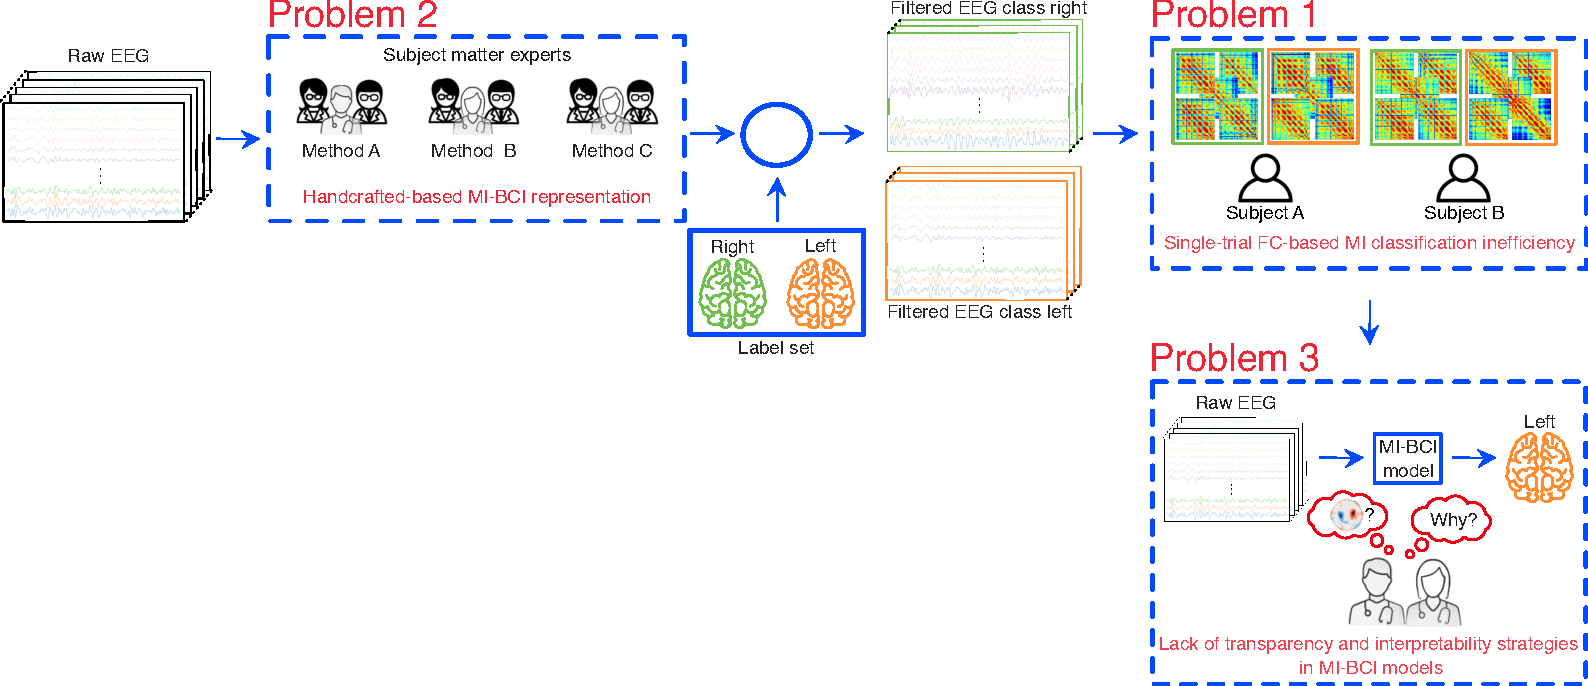
\includegraphics[width=1\linewidth]{../Tesis_document/Figures/problem_statement/general_problem.pdf}
        % \caption{Illustration of the three key challenges in FC EEG-based MI-BCI: noise and variability in single
        % trial FC estimators, handcrafted-based subject-specific EEG-based MI-BCI Representation, and the need for
        % model transparency}
    \end{figure}
\end{frame}

\begin{frame}{Single-Trial FC MI Classification Inefficiency}
    \begin{figure}[!ht]
        \centering
        \includegraphics[width=1\linewidth]{../Tesis_document/Figures/problem_statement/problem1_FV.pdf}
        % \caption{Single-trial FC-based MI classification inefficiency graphical scheme.}
    \end{figure}
\end{frame}

\begin{frame}{Handcrafted-based Subject-Specific EEG-based MI-BCI Representation}
    \begin{figure}[!ht]
        \centering
        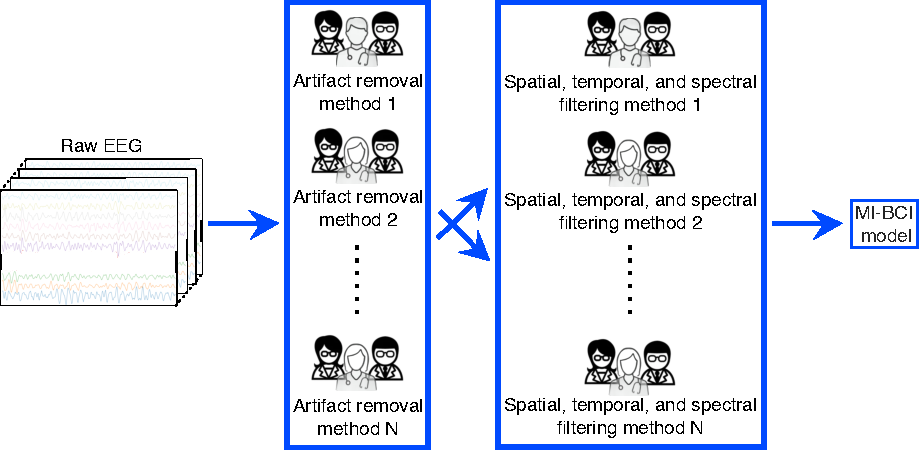
\includegraphics[width=0.9\linewidth]{../Tesis_document/Figures/problem_statement/problem2_VF.pdf}
        % \caption{llustration of challenges in EEG signal representation, including strategies for artifact removal and implementing spatial, temporal, and frequency filters.}
    \end{figure}
\end{frame}


\begin{frame}{Lack of Transparency and Interpretability Strategies in MI-BCI}
    \begin{figure}[!ht]
        \centering
        \includegraphics[width=1\linewidth]{../Tesis_document/Figures/problem_statement/problem3_FV.pdf}
        % \caption{Transparency and interpretability challenges in MI-BCI models graphical scheme.}
    \end{figure}
\end{frame}


\begin{frame}{Research question}
\centering
How can a single-trail FC be developed to manage non-stationary EEG subject-specific representations, handle spurious connectivities, and encode non-linear spatial, temporal, and spectral discriminative and interpretable MI patterns?
\end{frame}

\section{State of the art}
\subsection{Single-Trial FC in MI-BCI}

\begin{frame}{Functional Connectivity Estimators}
    \begin{columns}
        \column{0.58\textwidth}
        \centering
        \resizebox{1\textwidth}{!}{\includegraphics{../Tesis_document/Figures/state_of_art/sota1_EFC.pdf}}
        \column{0.42\textwidth}
        \begin{itemize}
            \item Orange shades indicate sensitivity to volume conduction (VC).
            \item Linear estimators are simple but may miss complex interactions, nonlinear ones capture them but are noise-sensitive \cite{gonzalez2020network}.
            \item Direct and Indirect connectivity achieve similar performance in MI, being indirect connectivity less sensitive to the VC~\cite{cao2022effective}
        \end{itemize}
    \end{columns}       
\end{frame}


\begin{frame}{Feature Extraction from FC}
    \centering
    \resizebox{0.95\linewidth}{!}{\includegraphics{../Tesis_document/Figures/state_of_art/sota1_FE.pdf}}
\end{frame}


\subsection{Subject-Specific EEG Representation for MI-BCI}


\begin{frame}{Input Formulation in Deep Learning}
    \begin{figure}[!ht]
        \centering
        \resizebox{0.85\linewidth}{!}{\includegraphics{../Tesis_document/Figures/state_of_art/sota2_input_v2.pdf}}
        % \caption{Functional connectivity estimators classified based on direct or indirect, time or frequency domain and linear or nonlinear. The varying shades of orange represent different sensitivities to volume conduction.}
    \end{figure}
\end{frame}


\begin{frame}{Deep Learning Architectures}
    \begin{figure}[!ht]
        \centering
        \resizebox{0.85\linewidth}{!}{\includegraphics{../Tesis_document/Figures/state_of_art/sota2_DLAV2.pdf}}
        % \caption{Functional connectivity estimators classified based on direct or indirect, time or frequency domain and linear or nonlinear. The varying shades of orange represent different sensitivities to volume conduction.}
    \end{figure}
\end{frame}

\subsection{Interpretability Strategies in MI-BCI}

\begin{frame}{Interpretability Strategies in MI-BCI}
    \begin{figure}[!ht]
        \centering
        \resizebox{0.9\linewidth}{!}{\includegraphics{../Tesis_document/Figures/state_of_art/sota3_methods.pdf}}
        % \caption{Functional connectivity estimators classified based on direct or indirect, time or frequency domain and linear or nonlinear. The varying shades of orange represent different sensitivities to volume conduction.}
    \end{figure}
\end{frame}

\section{Aims}

\begin{frame}{General Objective}
    To develop a single-trial indirect functional connectivity framework, accompanied by regularized deep learning approaches, to extract pertinent subject-specific non-linear spatio-temporal-frequency patterns from non-stationary EEG data, improving the MI-BCI system's accuracy and interpretability.
\end{frame}

\begin{frame}{Specific Objectives}
\centering
\begin{itemize}
    \setlength\itemsep{2em}
	\item[1] To develop a single-trial indirect FC for enhanced nonlinear feature extraction, preserving the spatio-temporal-frequency interpretability while favoring the classification performance in MI-BCI and avoiding spurious connectivities.
 
	\item[2] To extend the proposed single-trial FC within a deep learning scheme that handles artifacts and EEG representations, necessitating minimal preprocessing efforts from raw signals.
 
	\item[3] To develop a transparency and interpretability strategy dedicated to MI-BCI classification that emphasizes spatial-temporal-spectral pattern domains, incorporating a qualitative and quantitative relevance analysis assessment.
\end{itemize}
\end{frame}

\section{Outline and contributions}

\begin{frame}{Outline and contributions}
    \begin{figure}[h!]
        \centering
        \includegraphics[scale=0.65]{../Tesis_document/Figures/outline_and_contributions/general_contributions.pdf}
        % \caption{Schematic display of the main thesis contributions, including the single-trial FC estimator and feature extraction, an end-to-end approach from EEG representations to MI classification, and quantitative and qualitative strategies for model interpretation\label{fig:img_gen_outline}}
    \end{figure}
\end{frame}

\section{Datasets}

\begin{frame}{Datasets}
    \begin{table}[h]
        \centering
        \resizebox{0.9\textwidth}{!}{%
        \begin{tabular}{|c|c|c|c|c|c|c|c|}
            \hline
            \textbf{Dataset} & \textbf{Subjects} & \textbf{Trials} & \textbf{Paradigm} & \textbf{Classes} & \textbf{Channels} & \textbf{Sampling rate} \\
            \hline
            BCI Competition IV Dataset IIa (DBI MI)~\footnotemark[1] & 9 & 288 & Motor imagery & 2 & 22 & $250$Hz \\
            \hline
            Gamma Motor Execution Database (DBII ME)~\footnotemark[2] & 14 & 260 & Motor execution & 2 & 44 & $500$Hz \\
            \hline
            MI BCI EEG Giga Science Database (DBIII MI)~\footnotemark[3] & 50 & 200 & Motor imagery & 2 & 64 & $500$Hz \\
            \hline
        \end{tabular}
        }
    \end{table}
    \vspace{1em}
    \begin{columns}
        \column{0.33\textwidth}
            \centering
            \textbf{DBI MI}
            \vspace{2em}
            \resizebox{0.9\linewidth}{!}{\input{../Tesis_document/Figures/preliminaries/procedure_BCI2a.tikz}}
        \column{0.33\textwidth}
            \centering
            \textbf{DBII ME}
            \vspace{2em}
            \resizebox{1\linewidth}{!}{
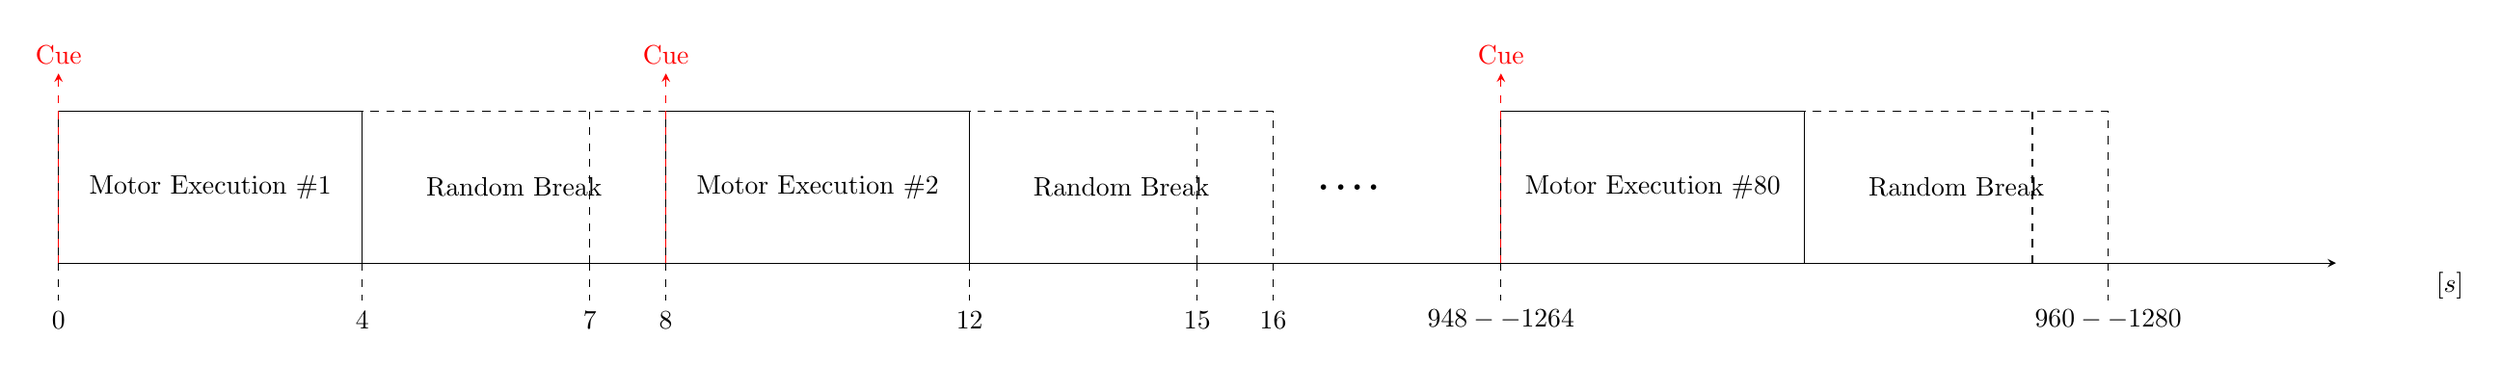
\begin{tikzpicture}
\draw[draw=black] (0,0) rectangle ++(4,2) node[pos=.5] {Motor Execution $\#1$};
\draw[dashed,draw=black] (4,0) rectangle ++(4,2) node[pos=.5] {Random Break};
\draw[dashed,draw=black] (7,0) -- (7,2) node[pos=1.5] {};

\draw[draw=black] (8,0) rectangle ++(4,2) node[pos=.5] {Motor Execution $\#2$};

\draw[dashed,draw=black] (12,0) rectangle ++(4,2) node[pos=.5] {Random Break};
\draw[dashed,draw=black] (15,0) -- (15,2) node[pos=1.5] {};

\draw[dashed,draw=black] (17,1) -- (17,1) node[pos=1.5] {\Huge{....}};


\draw[draw=black] (19,0) rectangle ++(4,2) node[pos=.5] {Motor Execution $\#80$};

\draw[dashed,draw=black] (23,0) rectangle ++(4,2) node[pos=.5] {Random Break};
\draw[dashed,draw=black] (26,0) -- (26,2) node[pos=1.5] {};


% \draw[draw=red] (2.5,-0.2) rectangle ++(2,1) node[pos=.5] {\textcolor{red}{\small{Analysis span}}};
% \draw[dashed,draw=red] (2.5,0) -- (2.5,-1) node[pos=1.5] {\textcolor{red}{$2.5$}};
% \draw[dashed,draw=red] (4.5,0) -- (4.5,-1) node[pos=1.5] {\textcolor{red}{$4.5$}};

\draw [-stealth](0,0) -- (30,0) node[below,pos=1.05] {$[s]$};

\draw[dashed,draw=black] (0,0) -- (0,-0.5) node[pos=1.5] {$0$};

\draw[-stealth,dashed,draw=red] (0,0) -- (0,2.5) node[pos=1.1] {\textcolor{red}{Cue}};
\draw[-stealth,dashed,draw=red] (8,0) -- (8,2.5) node[pos=1.1] {\textcolor{red}{Cue}};
\draw[-stealth,dashed,draw=red] (19,0) -- (19,2.5) node[pos=1.1] {\textcolor{red}{Cue}};


\draw[dashed,draw=black] (4,0) -- (4,-0.5) node[pos=1.5] {$4$};

\draw[dashed,draw=black] (7,0) -- (7,-0.5) node[pos=1.5] {$7$};
\draw[dashed,draw=black] (8,0) -- (8,-0.5) node[pos=1.5] {$8$};

\draw[dashed,draw=black] (12,0) -- (12,-0.5) node[pos=1.5] {$12$};
\draw[dashed,draw=black] (15,0) -- (15,-0.5) node[pos=1.5] {$15$};
\draw[dashed,draw=black] (16,0) -- (16,-0.5) node[pos=1.5] {$16$};

\draw[dashed,draw=black] (19,0) -- (19,-0.5) node[pos=1.5] {$948--1264$};

\draw[dashed,draw=black] (27,0) -- (27,-0.5) node[pos=1.5] {$960--1280$};

\end{tikzpicture}}
        \column{0.33\textwidth}
            \centering
            \textbf{DBIII MI}
            \vspace{2em}
            \includegraphics[width=0.9\linewidth]{../Tesis_document/Figures/preliminaries/protocol_giga.PNG}
    \end{columns}

    \footnotetext[1]{\url{http://www.bbci.de/competition/iv}}
    \footnotetext[2]{\url{https://gin.g-node.org/robintibor/high-gamma-dataset}}
    \footnotetext[3]{\url{http://gigadb.org/dataset/100295}}
\end{frame}

\section{Proposal and Results}

\subsection{Single-Trial Kernel-based Functional Connectivity for Enhanced Feature Extraction in EEG-based MI-BCI}

\begin{frame}[allowframebreaks]{Single-Trial Kernel-based Functional Connectivity}
    \begin{enumerate}
        \item \textbf{Wiener-Khinchin's theorem:} 
        \[
        R^{c}_{r}(\tau) = \int_{\varpi \in \Omega} \exp(j2\pi \tau \varpi) \, dP^{c}_{r}(\varpi),
        \]
        where $P^{c}_{r}(\varpi) \in \mathbb{R}[0,1]$ is the spectral distribution function.
        
        \item \textbf{Bochner's theorem:} 
        \[
        \kappa^{cc'}_{r}(\Delta_{x}) = \int_{\varpi \in \Omega} \exp(j2\pi \Delta_{x} \varpi) S^{cc'}_{r}(\varpi) \, d\varpi,
        \]
        where $\Delta_{x} = \mathbf{x}^{c}_{r} - \mathbf{x}^{c'}_{r}$ is the vector delay, $\varpi \subseteq \varOmega$ is the frequency domain that contains the bandwidth set of analysis $\varOmega$, and $S^{cc'}_{r}(\varpi)$ is the cross-spectral density.

        \item \textbf{Cross-spectral distribution:} 
        \[
        P^{cc'}_{r}(\varpi) = 2 \int_{\varpi \in \varOmega} \mathscr{F}\left\{\kappa(\mathbf{x}^{c}_{r}, \mathbf{x}^{c'}_{r}) \right\} \, d\varpi,
        \]
        where the notation $\mathscr{F}\{\cdot\}$ stands for the Fourier transform.

        \item \textbf{Kernel-based spectral distribution estimation:}
        \[
        \hat{P}^{cc'}_{r}(\mathbf{u}^{cc'},\kappa_x\left(\cdot;\sigma\right)) = \sum_{n=1}^{N_f}\sum_{w_t=1}^{N_t} u_{nw_t}^{cc'}\kappa_x\left(\mathbf{x}^{c}_{rnw_t},\mathbf{x}^{c'}_{rnw_t};\sigma\right),
        \]
        where $\mathbf{u}^{cc'} \in \mathbb{R}^{N_f N_t}$ is the spatio-temporal-frequency relevance vector.

        \item \textbf{Optimization Formulation:}
        {\scriptsize
        \[
        \mathbf{u}^* = \arg \min_{\mathbf{u}} \left\langle \sum_{r=1}^{R} \left\|\sum_{c,c'=1}^{N_c}\hat{P}^{cc'}_{r}(\mathbf{u}^{cc'},\kappa_x(\cdot;\sigma))-y_r\right\|^2_2 \right\rangle + \alpha \sum_{c,c'=1}^{N_c}\|\mathbf{u}^{cc'}\|_1 + \frac{1-\alpha}{2} \sum_{c,c'=1}^{N_c}\|\mathbf{u}^{cc'}\|_2 \quad :  \forall c < c',
        \]}

        where $\alpha \in \mathbb{R}^+$ is the regularization hyperparameter, $y_r$ is the label corresponding to the $r$-th trial, and $\| \cdot \|_q$ is the $\ell_q$-norm.
    \end{enumerate}
\end{frame}

\begin{frame}{Single-Trial Kernel-based Functional Connectivity proposal}
    \includegraphics[scale=0.5]{../Tesis_document/Figures/outline_and_contributions/contribution1_C.pdf}
\end{frame}

\begin{frame}{Experimental set-up}
    \begin{enumerate}
        \item Sliding window of length $\tau=[0.5,1.0,1.5,2.0]$\,{s}, and overlap of $75\%$.
        \item Frequency bands from $4$ Hz to $40$ Hz, window bandwidth of $4$Hz, and overlap of $50\%$.
        \item Gaussian kernel
        \[
        \kappa_x\left(\mathbf{x}^{c}_{rnw_t}, \mathbf{x}^{c'}_{rnw_t};\sigma\right) = \exp{\left( {-\|\mathbf{x}^{c}_{rnw_t}-\mathbf{x}^{c'}_{rnw_t}\|^2_2}/{2\sigma^2}\right)},
        \]
        \item We compare our proposal with {Cross-Correlation Coefficient} (CCF) and {Phase Lag Value} (PLV)
        \[
        \rho(\mathbf{x}^{c}_{rnw_t},\mathbf{x}^{c'}_{rnw_t}) ={\left<\mathbf{x}^{c}_{rnw_t},\mathbf{x}^{c'}_{rnw_t}\right>}
        \]
        \[
        \Delta\phi(\mathbf{x}^{c}_{rnw_t},\mathbf{x}^{c'}_{rnw_t}) = {|\exp(j(\phi_{rnw_t}^{c}-\phi_{rnw_t}^{c'}))|}
        \]
    \end{enumerate}
\end{frame}

% \begin{figure}[h!]
% \centering
% 	\hbox{\hspace{4.5cm} {PLV}\hspace{2.2cm} {CCF}\hspace{2cm} {KCS-FC}}
% 	\rotatebox{90}{ \quad\, \textbf{\tiny DBI MI}}
% 	\rotatebox{90}{\quad\,\tiny{Accuracy ($\%$)}}
% 	{\resizebox{\kerrwidth}{!}{\includegraphics[trim=85 100 80 80, clip]{../Tesis_document/Figures/Objective_1/taus_plv_BCI_MI.png}}}
% 	{\resizebox{\kerrwidth}{!}{\includegraphics[trim=85 100 80 80, clip]{../Tesis_document/Figures/Objective_1/taus_pearson_BCI_MI.png}}}
% 	{\resizebox{\kerrwidth}{!}{\includegraphics[trim=85 100 80 80, clip]{../Tesis_document/Figures/Objective_1/taus_gauss_BCI_MI.png}}}\\	
% 	\rotatebox{90}{ \quad\, \textbf{\tiny DBI MI-CSP} }
% 	\rotatebox{90}{\quad\,\tiny{Accuracy ($\%$)}}
% 	{\resizebox{\kerrwidth}{!}{\includegraphics[trim=85 100 80 80, clip]{../Tesis_document/Figures/Objective_1/taus_csp_plv_BCI_MI.png}}}
% 	{\resizebox{\kerrwidth}{!}{\includegraphics[trim=85 100 80 80, clip]{../Tesis_document/Figures/Objective_1/taus_csp_pearson_BCI_MI.png}}}
% 	{\resizebox{\kerrwidth}{!}{\includegraphics[trim=85 100 80 80, clip]{../Tesis_document/Figures/Objective_1/taus_csp_gauss_BCI_MI.png}}}
% \end{figure}  
    
% \begin{figure}[h!]
%     \centering
%         \hbox{\hspace{4.5cm} {PLV}\hspace{2.2cm} {CCF}\hspace{2cm} {KCS-FC}}
% 	\rotatebox{90}{ \quad\, \textbf{\tiny DBII ME}}
% 	\rotatebox{90}{\quad\,\tiny{Accuracy ($\%$)}}
% 	{\resizebox{\kerrwidth}{!}{\includegraphics[trim=85 100 80 80, clip]{../Tesis_document/Figures/Objective_1/taus_plv_HG_ME.png}}}
% 	{\resizebox{\kerrwidth}{!}{\includegraphics[trim=85 100 80 80, clip]{../Tesis_document/Figures/Objective_1/taus_pearson_HG_ME.png}}}
% 	{\resizebox{\kerrwidth}{!}{\includegraphics[trim=85 100 80 80, clip]{../Tesis_document/Figures/Objective_1/taus_gauss_HG_ME.png}}}\\
% 	\rotatebox{90}{ \quad\, \textbf{\tiny DBII ME-CSP}}
% 	\rotatebox{90}{ \quad\,\tiny{Accuracy ($\%$)}}
% 	{\resizebox{\kerrwidth}{!}{\includegraphics[trim=85 100 80 80, clip]{../Tesis_document/Figures/Objective_1/taus_CSP_plv_HG_ME.png}}}
% 	{\resizebox{\kerrwidth}{!}{\includegraphics[trim=85 100 80 80, clip]{../Tesis_document/Figures/Objective_1/taus_CSP_pearson_HG_ME.png}}}
% 	{\resizebox{\kerrwidth}{!}{\includegraphics[trim=85 100 80 80, clip]{../Tesis_document/Figures/Objective_1/taus_CSP_gauss_HG_ME.png}}}\\
% \end{figure}

\begin{frame}{Impact of Prior CSP Filtering}
    \def \kerrwidth {.3\linewidth}
    \begin{columns}
        \column{0.35\textwidth}
            \begin{itemize}
                \item PLV shows high variance and low accuracy..
                \item KCS-FC outperforms other FC measures, with less variance in accuracy across subjects.
                \item CSP accuracy drops at $\tau=0.5$ due to its reliance on FC estimation, with less information leading to poorer estimates.
            \end{itemize}
        \column{0.65\textwidth}
            \begin{figure}[h!]
                \centering
                \hbox{\hspace{1.7cm} {PLV}\hspace{2.2cm} {CCF}\hspace{2cm} {KCS-FC}}	
                \rotatebox{90}{ \quad\, \textbf{\tiny DBIII MI}}
                \rotatebox{90}{ \quad\,\tiny{Accuracy ($\%$)}}
                \resizebox{\kerrwidth}{!}{\includegraphics[trim=85 100 80 80, clip]{../Tesis_document/Figures/Objective_1/taus_plv_giga_MI.png}}
                \resizebox{\kerrwidth}{!}{\includegraphics[trim=85 100 80 80, clip]{../Tesis_document/Figures/Objective_1/taus_pearson_giga_MI.png}}
                \resizebox{\kerrwidth}{!}{\includegraphics[trim=85 100 80 80, clip]{../Tesis_document/Figures/Objective_1/taus_gauss_giga_MI.png}}\\
                \rotatebox{90}{\quad \textbf{\tiny DBIII MI-CSP}}
                \rotatebox{90}{ \quad\,\tiny{Accuracy ($\%$)}}
                \resizebox{\kerrwidth}{!}{\includegraphics[trim=85 100 80 80, clip]{../Tesis_document/Figures/Objective_1/taus_csp_plv_giga_MI.png}}
                \resizebox{\kerrwidth}{!}{\includegraphics[trim=85 100 80 80, clip]{../Tesis_document/Figures/Objective_1/taus_csp_pearson_giga_MI.png}}
                \resizebox{\kerrwidth}{!}{\includegraphics[trim=85 100 80 80, clip]{../Tesis_document/Figures/Objective_1/taus_csp_gauss_giga_MI.png}}\\
            \end{figure}
    \end{columns}
\end{frame}


\begin{frame}{Influence of Sliding Windows}
\begin{figure}[h!]
    \centering
    \resizebox{0.5\linewidth}{!}{
        \begin{tabular}{c}
            \rotatebox{90}{\qquad \quad\, \textbf{DBI-MI}}
            \rotatebox{90}{\qquad \quad\, \footnotesize{Accuracy ($\%$)}}
            \includegraphics[width=0.9\linewidth]{../Tesis_document/Figures/Objective_1/acc_regularizacionDBII} \\
            \rotatebox{90}{\qquad \quad\, \textbf{DBII-ME}}
            \rotatebox{90}{\qquad \quad\, \footnotesize{Accuracy ($\%$)}}
            \includegraphics[width=0.9\linewidth]{../Tesis_document/Figures/Objective_1/acc_regularizacionHG_ME} \\
            \rotatebox{90}{\qquad \quad\, \textbf{DBIII-MI}}
            \rotatebox{90}{\qquad \quad\, \footnotesize{Accuracy ($\%$)}}
            \includegraphics[width=0.9\linewidth]{../Tesis_document/Figures/Objective_1/acc_regularizacion} \\
            \hbox{\hspace{2cm} \textbf{Window length}}
        \end{tabular}
    }
\end{figure}
\end{frame}

\begin{frame}[allowframebreaks]{Classifier Accuracy of Individuals}
\def \kerrwidth {0.35\linewidth} 
\begin{figure}[h!]
	\hbox{\hspace{4.5cm} \textbf{DBII-ME}\hspace{4cm} \textbf{DBIII-MI}}
	\rotatebox{90}{\qquad \,\footnotesize{Window size}}
	\rotatebox{90}{\qquad \, \footnotesize{$\tau= 2.0$\,{s}}}
	\rotatebox{90}{\qquad \,\tiny{Accuracy ($\%$)}}
	{\resizebox{\kerrwidth }{!}{\includegraphics{../Tesis_document/Figures/Objective_1/ptau2-hg-Me}}}
	{\resizebox{\kerrwidth }{!}{\includegraphics{../Tesis_document/Figures/Objective_1/ptau2-giga-Mi}}} \\
	\rotatebox{90}{\qquad \,\footnotesize{Window size}}	
	\rotatebox{90}{\qquad \, \footnotesize{$\tau= 1.5$\,{s}}}
	\rotatebox{90}{\qquad \,\tiny{Accuracy ($\%$)}}
	{\resizebox{\kerrwidth }{!}{\includegraphics{../Tesis_document/Figures/Objective_1/ptau1_5-hg-Me}}}
	{\resizebox{\kerrwidth }{!}{\includegraphics{../Tesis_document/Figures/Objective_1/ptau1_5-giga-Mi}}}\\
    \hbox{\hspace{4.5cm} \footnotesize{Subject id}\hspace{4cm} \footnotesize{Subject id}}
\end{figure}
\begin{figure}[h!]
    \hbox{\hspace{4.5cm} \textbf{DBII-ME}\hspace{4cm} \textbf{DBIII-MI}}
	\rotatebox{90}{\qquad \,\footnotesize{Window size}}	
	\rotatebox{90}{\qquad \, \footnotesize{$\tau= 1.0$\,{s}}}
	\rotatebox{90}{\qquad \,\tiny{Accuracy ($\%$)}}
	{\resizebox{\kerrwidth }{!}{\includegraphics{../Tesis_document/Figures/Objective_1/ptau1-hg-Me}}}
	{\resizebox{\kerrwidth }{!}{\includegraphics{../Tesis_document/Figures/Objective_1/ptau1-giga-Mi}}}\\
	\rotatebox{90}{\qquad \,\footnotesize{Window size}}	
	\rotatebox{90}{\qquad \, \footnotesize{$\tau= 0.5$\,{s}}}
	\rotatebox{90}{\qquad \,\tiny{Accuracy ($\%$)}}
	{\resizebox{\kerrwidth }{!}{\includegraphics{../Tesis_document/Figures/Objective_1/ptau0_5-hg-Me}}}
	{\resizebox{\kerrwidth }{!}{\includegraphics{../Tesis_document/Figures/Objective_1/ptau0_5-giga-Mi}}} \\
	\hbox{\hspace{4.5cm} \footnotesize{Subject id}\hspace{4cm} \footnotesize{Subject id}}
\end{figure}
\end{frame}

\begin{frame}{Interpretation of Subject Clusters}
    \def \kerrwidthME {.32\linewidth}
    \def \kerrwidthMI {.55\linewidth}
    \begin{figure}[h!]    
        \centering
        \resizebox{0.7\linewidth}{!}{
            \begin{tabular}{c c c}
                & \textbf{DBII~ME} & \textbf{DBIII~MI} \\
                \rotatebox{90}{\footnotesize{PLV}} 
                \rotatebox{90}{\footnotesize{Window size}} &
                \includegraphics[width=\kerrwidthME]{../Tesis_document/Figures/Objective_1/plv_hg} &
                \includegraphics[width=\kerrwidthMI]{../Tesis_document/Figures/Objective_1/plv_giga} \\
                \rotatebox{90}{\footnotesize{CCF}} 
                \rotatebox{90}{\footnotesize{Window size}} &
                \includegraphics[width=\kerrwidthME]{../Tesis_document/Figures/Objective_1/pearson_hg} &
                \includegraphics[width=\kerrwidthMI]{../Tesis_document/Figures/Objective_1/pearson_giga} \\
                \rotatebox{90}{\footnotesize{KCS-FC}} 
                \rotatebox{90}{\footnotesize{Window size}} &
                \includegraphics[width=\kerrwidthME]{../Tesis_document/Figures/Objective_1/gauss_hg} &
                \includegraphics[width=\kerrwidthMI]{../Tesis_document/Figures/Objective_1/gauss_giga} \\
                & \footnotesize{Subject id} & \footnotesize{Subject id}
            \end{tabular}
        }
    \end{figure} 
\end{frame}

\begin{frame}{asd}
    \nointerlineskip
\def \kerrwidth {0.15\linewidth}
\def \kerrwidthc {0.022\linewidth}
\def \kerrg {0.12\linewidth}
\def \kerrgg {0.05\linewidth}
\def \kerrggg {0.04\linewidth}
%\begingroup
\tabcolsep = 2.0pt
\def\arraystretch{1.0}
\begin{figure}[h!]
%\widefigure
\scalebox{0.6}[0.6]{\begin{tabular}{cccccccc}
\centering
& & \textbf{DBII~ME}& & & \textbf{DBIII~MI}&\\
\cmidrule{2-7}
& {I} & {II}&{III}&{I} & {II}&{III}&
\multirow{6}{*}{{\includegraphics[trim=660 0 0 0, clip,scale=0.35]{../Tesis_document/Figures/Objective_1/Cxsbj1hg-gaussacc95.28.eps}}}\\
\cmidrule{2-7}
& \textbf{$84.13\%$}& \textbf{$74.91\%$} & \textbf{$64.21\%$} & \textbf{$72.2\%$} & \textbf{$68.76\%$} & \textbf{$55.94\%$}&\\
{\rotatebox{90}{\hspace{7mm} {PLV}}}&{\resizebox{\kerrwidth}{!}{\includegraphics[trim=100 120 90 90, clip]{../Tesis_document/Figures/Objective_1/Cxsbj1hg-plvacc84.13.eps}}}&
	{\resizebox{\kerrwidth}{!}{\includegraphics[trim=100 120 90 90, clip]{../Tesis_document/Figures/Objective_1/Cxsbj2hg-plvacc74.91.eps}}}&
	{\resizebox{\kerrwidth}{!}{\includegraphics[trim=100 120 90 90, clip]{../Tesis_document/Figures/Objective_1/Cxsbj3hg-plvacc64.21.eps}}}&
	{\resizebox{\kerrwidth}{!}{\includegraphics[trim=100 120 90 90, clip]{../Tesis_document/Figures/Objective_1/Cxsbj1plvacc72.2.eps}}}&
	{\resizebox{\kerrwidth}{!}{\includegraphics[trim=100 120 90 90, clip]{../Tesis_document/Figures/Objective_1/Cxsbj2plvacc68.76.eps}}}&
	{\resizebox{\kerrwidth}{!}{\includegraphics[trim=100 120 90 90, clip]{../Tesis_document/Figures/Objective_1/Cxsbj3plvacc55.94.eps}}}&\\
	& \textbf{$90.06\%$} & \textbf{$79.35\%$} & \textbf{$70.59\%$} &  \textbf{$76.67\%$} & \textbf{$64.62\%$} & \textbf{$60.69\%$}&\\
	\rotatebox{90}{\hspace{7mm} {CCF}}&
	{\resizebox{\kerrwidth}{!}{\includegraphics[trim=100 120 90 90, clip]{../Tesis_document/Figures/Objective_1/Cxsbj1hg-pearsonacc90.06.eps}}}&
	{\resizebox{\kerrwidth}{!}{\includegraphics[trim=100 120 90 90, clip]{../Tesis_document/Figures/Objective_1/Cxsbj2hg-pearsonacc79.35.eps}}}&
	{\resizebox{\kerrwidth}{!}{\includegraphics[trim=100 120 90 90, clip]{../Tesis_document/Figures/Objective_1/Cxsbj3hg-pearsonacc70.59.eps}}}&
	{\resizebox{\kerrwidth}{!}{\includegraphics[trim=100 120 90 90, clip]{../Tesis_document/Figures/Objective_1/Cxsbj1pearsonacc76.67.eps}}}&
	{\resizebox{\kerrwidth}{!}{\includegraphics[trim=100 120 90 90, clip]{../Tesis_document/Figures/Objective_1/Cxsbj2pearsonacc64.62.eps}}}&
	{\resizebox{\kerrwidth}{!}{\includegraphics[trim=100 120 90 90, clip]{../Tesis_document/Figures/Objective_1/Cxsbj3pearsonacc60.69.eps}}}&\\
	& \textbf{$\mathbf{95.28}\%$}& \textbf{$\mathbf{81.16}\%$}& \textbf{$\mathbf{76.09}\%$}& \textbf{$\mathbf{86.85}\%$}& \textbf{$\mathbf{68.93}\%$}& \textbf{$\mathbf{64.4}5\%$}&\\
	\rotatebox{90}{\hspace{7mm} {KCS-FC}}&
	{\resizebox{\kerrwidth}{!}{\includegraphics[trim=100 120 90 90, clip]{../Tesis_document/Figures/Objective_1/Cxsbj1hg-gaussacc95.28.eps}}}&
	{\resizebox{\kerrwidth}{!}{\includegraphics[trim=100 120 90 90, clip]{../Tesis_document/Figures/Objective_1/Cxsbj2hg-gaussacc81.16.eps}}}&
	{\resizebox{\kerrwidth}{!}{\includegraphics[trim=100 120 90 90, clip]{../Tesis_document/Figures/Objective_1/Cxsbj3hg-gaussacc76.09.eps}}}&
	{\resizebox{\kerrwidth}{!}{\includegraphics[trim=100 120 90 90, clip]{../Tesis_document/Figures/Objective_1/Cxsbj1gaussacc86.85.eps}}}&
	{\resizebox{\kerrwidth}{!}{\includegraphics[trim=100 120 90 90, clip]{../Tesis_document/Figures/Objective_1/Cxsbj2gaussacc68.93.eps}}}&
	{\resizebox{\kerrwidth}{!}{\includegraphics[trim=100 120 90 90, clip]{../Tesis_document/Figures/Objective_1/Cxsbj3gaussacc64.45.eps}}}&\\
	&\multicolumn{6}{c}{\resizebox{0.85\linewidth}{!}{\includegraphics[trim=0 0 50 600, clip]{../Tesis_document/Figures/Objective_1/Cxsbj1hg-gaussacc95.28.eps}}}&
\end{tabular}}
\end{figure}
\end{frame}


\begin{frame}{Classifier accuracy comparison of FC approaches}
    \begin{table}[h!]    
    \resizebox{0.8\columnwidth}{!}{
    \begin{tabular}{cccccc}
        \toprule
            \textbf{Data}& \textbf{Time Window} & \textbf{Filter Band} & \textbf{Interpretation} & \textbf{Feature Extraction}  & \textbf{Accuracy} (\%)\\
            \midrule
            {\multirow{4}{*}{\rotatebox[origin=c]{90}{{DBI-MI}%MDPI: please confirm the text direction. We confirm.
    }}} &
            \checkmark&\checkmark&\checkmark&TSGSP~\cite{Zhang2018}&\textbf{82.50} $\pm$ \textbf{12.2}\\
            &-&-&\checkmark&STR connectivity~\cite{rodrigue2019}&69.56$\pm$15.02\\
            & \checkmark & - & \checkmark & Renyi's $\alpha$-entropy~\cite{de2019data} & 72.40 $\pm$ 6.50\\					
            &\checkmark&\checkmark&\checkmark&{Proposed KCS-FC}& {81.92} $\pm$ {9.44}\\
            \midrule	
            {\multirow{4}{*}{\rotatebox[origin=c]{90}{DBIII-MI}}} &		
            - &\checkmark&\checkmark & CSP~\cite{cho2017eeg}&67.60 $\pm$ 13.17\\
            &\checkmark&\checkmark&-&OPTICAL~\cite{kumar2019brain}&68.19 $\pm$ 9.36\\
            &-&-&\checkmark&STR connectivity~\cite{rodrigue2019}&62.00 $\pm$ 13.00\\	
            &\checkmark&\checkmark&\checkmark&{Proposed KCS-FC}&\textbf{74.12} $\pm$ \textbf{12.13} \\\bottomrule
        \end{tabular}
     }
    \end{table}
\end{frame}

\subsection{KCS-FCnet: Kernel Cross-Spectral Functional Connectivity Network for Automatic EEG Representation in MI-BCI}

\begin{frame}[allowframebreaks]{Kernel Cross-Spectral Functional Connectivity Network}
    \begin{enumerate}
        \item \textbf{1-D convolutional feature extraction and Gaussian pairwise similarity:}
        \[
            \hat{\mat{P}}_{r}(\ve{w}_f)  = \tilde{K}(\cdot;\sigma) \circ \varphi(\mat{X}_r; \ve{w}_f), 
        \]
        where $\tilde{K}(\mat{\tilde{X}}_r;\sigma) = \left[ \mat{K}_{r1} , \mat{K}_{r2}, \cdots,\mat{K}_{rf},\cdots, \mat{K}_{rN_f} \right]$ and  $\mat{K}_{rf}$ is defined as:
        \[
            \mat{K}_{rf} = \begin{bmatrix}
                \kappa_{x}(\ve{x}^{1}_{rf}, \ve{x}^{1}_{rf}; \sigma) & \kappa_{x}(\ve{x}^{1}_{rf}, \ve{x}^{2}_{rf}; \sigma) & \cdots & \kappa_{x}(\ve{x}^{1}_{rf}, \ve{x}^{N_c}_{rf}; \sigma) \\
                \kappa_{x}(\ve{x}^{2}_{rf}, \ve{x}^{1}_{rf}; \sigma) & \kappa_{x}(\ve{x}^{2}_{rf}, \ve{x}^{2}_{rf}; \sigma) & \cdots & \kappa_{x}(\ve{x}^{2}_{rf}, \ve{x}^{N_c}_{rf}; \sigma) \\
                \vdots & \vdots & \ddots & \vdots \\
                \kappa_{x}(\ve{x}^{N_c}_{rf}, \ve{x}^{1}_{rf}; \sigma) & \kappa_{x}(\ve{x}^{N_c}_{rf}, \ve{x}^{2}_{rf}; \sigma) & \cdots & \kappa_{x}(\ve{x}^{N_c}_{rf}, \ve{x}^{N_c}_{rf}; \sigma).
            \end{bmatrix}
        \]
        \item \textbf{Average functional connectivity measure:}
        \[
            \tilde{\mat{P}}_r  = \operatorname{AvgPooling}_{f} \left(\hat{\mat{P}}_{r}(\ve{w}_f)\right),
        \]
        \item \textbf{Vectorized version of} $\tilde{\mat{P}}_r$ \textbf{:}
        \[
            \overline{\ve{p}}_r = \left[\tilde{p}_r^{12}, \tilde{p}_r^{13}, \cdots, \tilde{p}_r^{cc'}, \cdots, \tilde{p}_r^{(N_c-1) N_c} \right]; \forall c<c',
        \]
        \item \textbf{Optimization Formulation:}
        \[
            \Theta^{*} = \underset{\Theta}{\arg\,\min} \quad \promeddd{r}{\mathcal{L}(\ve{y}_r,\hat{\ve{y}}_r|\Theta); \forall r\in\{1,2,\dots,R\}},
        \]
        where $\mathcal{L} \{\cdot\}$ is a given loss function, and $\hat{\ve{y}}_r = \mathrm{softmax}\left(\mat{V}\overline{\ve{p}}_r + \ve{b}\right)$
    \end{enumerate}
\end{frame}

\begin{frame}{Kernel Cross-Spectral Functional Connectivity Network proposal}
    \centering
    \includegraphics[scale=0.5]{../Tesis_document/Figures/outline_and_contributions/contribution2.pdf}
\end{frame}

\begin{frame}{Kernel Cross-Spectral Functional Connectivity Network architecture}
    \begin{table}[H]
		\centering
        \resizebox{0.7\textwidth}{!}{
		\begin{tabularx}{\textwidth}{lcc}
			\hline
			\textbf{Layer}     & \textbf{Output Dimension}           & \textbf{Params.}                                                       \\ \midrule
			Input              & $N_c \times N_t \times 1$                 & $\cdot$                                                                  \\
			Conv2D             & $N_c \times (N_t - \Delta_t + 1) \times N_f$     & \begin{tabular}[c]{@{}c@{}}max norm = 2.0, kernel size = (1, $\Delta_t$)\\ Stride size = (1, 1), Bias = False\end{tabular} \\
			BatchNormalization & $N_c \times (N_t - \Delta_t + 1) \times N_f$     & $\cdot$                                                                  \\ \midrule
			\multicolumn{3}{c}{ELU activation}                                                                                               \\ \midrule
			KCS-FCblock           & $N_f \times (N_c \cdot (N_c-1)/2) \times 1$ & $\cdot$                                                                  \\
			AveragePooling2D   & $1 \times (N_c \cdot (N_c-1)/2) \times 1$  & $\cdot$                                                                  \\
			BatchNormalization & $1 \times (N_c \cdot (N_c-1)/2) \times 1$  & $\cdot$                                                                  \\ \midrule
			\multicolumn{3}{c}{ELU activation}                                                                                               \\ \midrule
			Flatten            & $N_c \cdot (N_c-1)/2$                  & $\cdot$                                                                  \\
			Dropout            & $N_c \cdot (N_c-1)/2$                   & Dropout rate = 0.5                                                    \\
			Dense              & $N_y$                                  & max norm = 0.5                                                        \\ \midrule
			\multicolumn{3}{c}{Softmax}                                                                                                      \\ \midrule
		\end{tabularx}
        }
	\end{table}

\end{frame}

\begin{frame}{Experimental set-up}
    \begin{enumerate}
        \item \textbf{Raw EEG Preprocessing:} 
        \begin{itemize}
            \item Database used DBIII MI
            \item Donwsampling from $512$ Hz to $128$ Hz. 
            \item Filtering from $4$ Hz to $40$ Hz. 
            \item Records clipped from $0.5$ s to $2.5$ s post cue.
        \end{itemize}
        \item \textbf{KCS-FCnet Training:}
        \begin{itemize}
            \item Data split using 5-fold 80-20 scheme.
            \item 1-D convolutional kernel length set to $20$ as in \cite{lawhern2018eegnet}
            \item Number of filters were searched within the set $\{2,3,4\}$
        \end{itemize}
        \item \textbf{Group-Level Analysis:}
        \begin{itemize}
            \item Scaled scoring matrix with subjects and accuracy, Cohen's kappa, AUC.
            \item Cluster subjects in three groups based on base line EEGnet.
            \item PCA was used to reduce the dimensions to two, enabling us to plot it.
        \end{itemize}
    \end{enumerate}
\end{frame}

\begin{frame}{Subject Dependent and Group Analysis Results I}
    \centering
    \resizebox{0.7\linewidth}{!}{% This file was created with tikzplotlib v0.10.1.
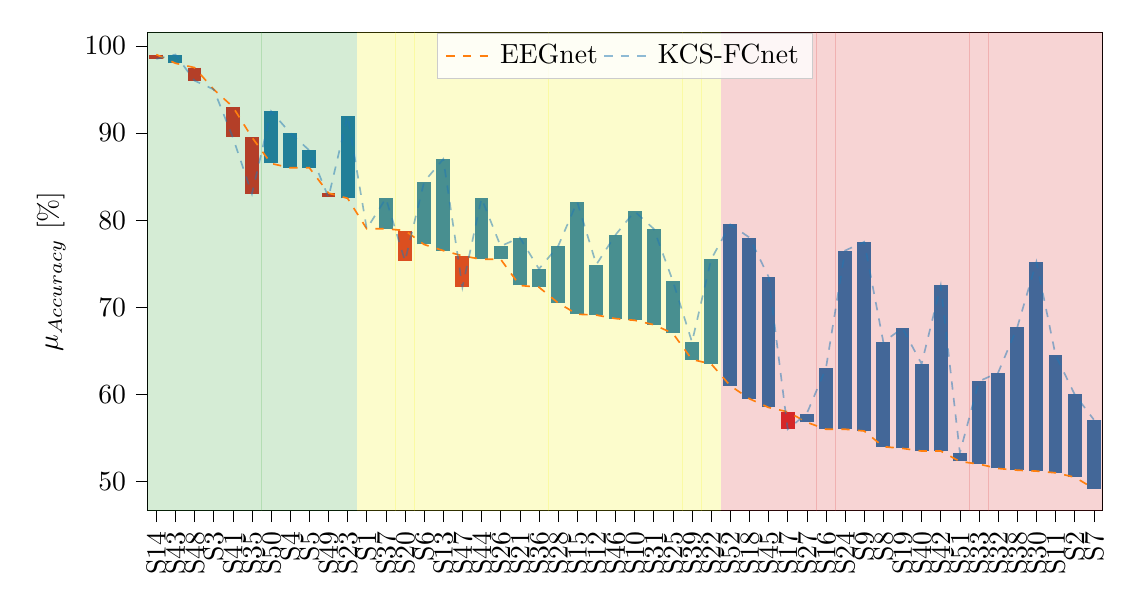
\begin{tikzpicture}

\definecolor{crimson2143940}{RGB}{214,39,40}
\definecolor{darkgray176}{RGB}{176,176,176}
\definecolor{darkorange25512714}{RGB}{255,127,14}
\definecolor{lightgray204}{RGB}{204,204,204}
\definecolor{steelblue31119180}{RGB}{31,119,180}

\definecolor{green}{RGB}{44,160,44}
\definecolor{yellow}{RGB}{240,240,0}
\definecolor{red}{RGB}{214,39,40}

\begin{axis}[
legend cell align={left},
legend cell align={left},
legend columns=2,
legend columns=2,
legend style={
  fill opacity=0.8,
  draw opacity=1,
  text opacity=1,
  at={(0.5,1)},
  anchor=north,
  draw=lightgray204
},
legend style={
  fill opacity=0.8,
  draw opacity=1,
  text opacity=1,
  at={(0.5,1)},
  anchor=north,
  draw=lightgray204
},
tick align=outside,
tick pos=left,
x grid style={darkgray176},
xmin=-0.45, xmax=49.45,
xtick style={color=black},
xtick={0,1,2,3,4,5,6,7,8,9,10,11,12,13,14,15,16,17,18,19,20,21,22,23,24,25,26,27,28,29,30,31,32,33,34,35,36,37,38,39,40,41,42,43,44,45,46,47,48,49},
xticklabel style={rotate=90.0},
xticklabels={
  S14,
  S43,
  S48,
  S3,
  S41,
  S35,
  S50,
  S4,
  S5,
  S49,
  S23,
  S1,
  S37,
  S20,
  S6,
  S13,
  S47,
  S44,
  S26,
  S21,
  S36,
  S28,
  S15,
  S12,
  S46,
  S10,
  S31,
  S25,
  S39,
  S22,
  S52,
  S18,
  S45,
  S17,
  S27,
  S16,
  S24,
  S9,
  S8,
  S19,
  S40,
  S42,
  S51,
  S33,
  S32,
  S38,
  S30,
  S11,
  S2,
  S7
},
y grid style={darkgray176},
ylabel={\(\displaystyle \mu_{Accuracy}\) [\%]},
ymin=46.71, ymax=101.49,
ytick style={color=black},
% only scale the axis, not the axis including the ticks and labels
scale only axis=true,
% set `width' and `height' to the desired values
width=\textwidth,
height=0.5\textwidth,
]

\path [draw=steelblue31119180, line width=5pt]
(axis cs:1,98)
--(axis cs:1,99);

\path [draw=steelblue31119180, line width=5pt]
(axis cs:3,95)
--(axis cs:3,95);



\path [draw=steelblue31119180, line width=5pt]
(axis cs:6,86.5)
--(axis cs:6,92.5);

\path [draw=steelblue31119180, line width=5pt]
(axis cs:7,86)
--(axis cs:7,90);

\path [draw=steelblue31119180, line width=5pt]
(axis cs:8,86)
--(axis cs:8,88);

\path [draw=steelblue31119180, line width=5pt]
(axis cs:10,82.5)
--(axis cs:10,92);

\path [draw=steelblue31119180, line width=5pt]
(axis cs:11,79)
--(axis cs:11,79);

\path [draw=steelblue31119180, line width=5pt]
(axis cs:12,79)
--(axis cs:12,82.5);

\path [draw=steelblue31119180, line width=5pt]
(axis cs:14,77.2)
--(axis cs:14,84.4);

\path [draw=steelblue31119180, line width=5pt]
(axis cs:15,76.5)
--(axis cs:15,87);

\path [draw=steelblue31119180, line width=5pt]
(axis cs:17,75.5)
--(axis cs:17,82.5);

\path [draw=steelblue31119180, line width=5pt]
(axis cs:18,75.5)
--(axis cs:18,77);

\path [draw=steelblue31119180, line width=5pt]
(axis cs:19,72.5)
--(axis cs:19,78);

\path [draw=steelblue31119180, line width=5pt]
(axis cs:20,72.3)
--(axis cs:20,74.4);

\path [draw=steelblue31119180, line width=5pt]
(axis cs:21,70.5)
--(axis cs:21,77);

\path [draw=steelblue31119180, line width=5pt]
(axis cs:22,69.2)
--(axis cs:22,82.1);

\path [draw=steelblue31119180, line width=5pt]
(axis cs:23,69.1)
--(axis cs:23,74.9);

\path [draw=steelblue31119180, line width=5pt]
(axis cs:24,68.7)
--(axis cs:24,78.3);

\path [draw=steelblue31119180, line width=5pt]
(axis cs:25,68.5)
--(axis cs:25,81);

\path [draw=steelblue31119180, line width=5pt]
(axis cs:26,68)
--(axis cs:26,79);

\path [draw=steelblue31119180, line width=5pt]
(axis cs:27,67)
--(axis cs:27,73);

\path [draw=steelblue31119180, line width=5pt]
(axis cs:28,64)
--(axis cs:28,66);

\path [draw=steelblue31119180, line width=5pt]
(axis cs:29,63.5)
--(axis cs:29,75.5);

\path [draw=steelblue31119180, line width=5pt]
(axis cs:30,61)
--(axis cs:30,79.5);

\path [draw=steelblue31119180, line width=5pt]
(axis cs:31,59.5)
--(axis cs:31,78);

\path [draw=steelblue31119180, line width=5pt]
(axis cs:32,58.5)
--(axis cs:32,73.5);

\path [draw=steelblue31119180, line width=5pt]
(axis cs:34,56.8)
--(axis cs:34,57.8);

\path [draw=steelblue31119180, line width=5pt]
(axis cs:35,56)
--(axis cs:35,63);

\path [draw=steelblue31119180, line width=5pt]
(axis cs:36,56)
--(axis cs:36,76.5);

\path [draw=steelblue31119180, line width=5pt]
(axis cs:37,55.8)
--(axis cs:37,77.5);

\path [draw=steelblue31119180, line width=5pt]
(axis cs:38,54)
--(axis cs:38,66);

\path [draw=steelblue31119180, line width=5pt]
(axis cs:39,53.8)
--(axis cs:39,67.6);

\path [draw=steelblue31119180, line width=5pt]
(axis cs:40,53.5)
--(axis cs:40,63.5);

\path [draw=steelblue31119180, line width=5pt]
(axis cs:41,53.5)
--(axis cs:41,72.5);

\path [draw=steelblue31119180, line width=5pt]
(axis cs:42,52.3)
--(axis cs:42,53.3);

\path [draw=steelblue31119180, line width=5pt]
(axis cs:43,52)
--(axis cs:43,61.5);

\path [draw=steelblue31119180, line width=5pt]
(axis cs:44,51.5)
--(axis cs:44,62.5);

\path [draw=steelblue31119180, line width=5pt]
(axis cs:45,51.3)
--(axis cs:45,67.7);

\path [draw=steelblue31119180, line width=5pt]
(axis cs:46,51.2)
--(axis cs:46,75.2);

\path [draw=steelblue31119180, line width=5pt]
(axis cs:47,51)
--(axis cs:47,64.5);

\path [draw=steelblue31119180, line width=5pt]
(axis cs:48,50.5)
--(axis cs:48,60);

\path [draw=steelblue31119180, line width=5pt]
(axis cs:49,49.2)
--(axis cs:49,57.1);

\path [draw=crimson2143940, line width=5pt]
(axis cs:0,99)
--(axis cs:0,98.5);

\path [draw=crimson2143940, line width=5pt]
(axis cs:2,97.5)
--(axis cs:2,96);

\path [draw=crimson2143940, line width=5pt]
(axis cs:4,93)
--(axis cs:4,89.5);

\path [draw=crimson2143940, line width=5pt]
(axis cs:5,89.5)
--(axis cs:5,83);

\path [draw=crimson2143940, line width=5pt]
(axis cs:9,83.1)
--(axis cs:9,82.6);

\path [draw=crimson2143940, line width=5pt]
(axis cs:13,78.8)
--(axis cs:13,75.3);

\path [draw=crimson2143940, line width=5pt]
(axis cs:16,75.9)
--(axis cs:16,72.3);

\path [draw=crimson2143940, line width=5pt]
(axis cs:33,58)
--(axis cs:33,56);

\path [draw=green, opacity=0.2, line width=7pt]
(axis cs:1,45)
--(axis cs:1,105);

\path [draw=green, opacity=0.2, line width=7pt]
(axis cs:0,45)
--(axis cs:0,105);

\path [draw=green, opacity=0.2, line width=7pt]
(axis cs:2,45)
--(axis cs:2,105);

\path [draw=green, opacity=0.2, line width=7pt]
(axis cs:3,45)
--(axis cs:3,105);

\path [draw=green, opacity=0.2, line width=7pt]
(axis cs:4,45)
--(axis cs:4,105);

\path [draw=green, opacity=0.2, line width=7pt]
(axis cs:5,45)
--(axis cs:5,105);

\path [draw=green, opacity=0.2, line width=7pt]
(axis cs:6,45)
--(axis cs:6,105);

\path [draw=green, opacity=0.2, line width=7pt]
(axis cs:7,45)
--(axis cs:7,105);

\path [draw=green, opacity=0.2, line width=7pt]
(axis cs:8,45)
--(axis cs:8,105);

\path [draw=green, opacity=0.2, line width=7pt]
(axis cs:9,45)
--(axis cs:9,105);

\path [draw=green, opacity=0.2, line width=7pt]
(axis cs:10,45)
--(axis cs:10,105);

\path [draw=yellow, opacity=0.2, line width=7pt]
(axis cs:11,45)
--(axis cs:11,105);

\path [draw=yellow, opacity=0.2, line width=7pt]
(axis cs:12,45)
--(axis cs:12,105);

\path [draw=yellow, opacity=0.2, line width=7pt]
(axis cs:13,45)
--(axis cs:13,105);

\path [draw=yellow, opacity=0.2, line width=7pt]
(axis cs:14,45)
--(axis cs:14,105);

\path [draw=yellow, opacity=0.2, line width=7pt]
(axis cs:15,45)
--(axis cs:15,105);

\path [draw=yellow, opacity=0.2, line width=7pt]
(axis cs:16,45)
--(axis cs:16,105);

\path [draw=yellow, opacity=0.2, line width=7pt]
(axis cs:17,45)
--(axis cs:17,105);

\path [draw=yellow, opacity=0.2, line width=7pt]
(axis cs:18,45)
--(axis cs:18,105);

\path [draw=yellow, opacity=0.2, line width=7pt]
(axis cs:19,45)
--(axis cs:19,105);

\path [draw=yellow, opacity=0.2, line width=7pt]
(axis cs:20,45)
--(axis cs:20,105);

\path [draw=yellow, opacity=0.2, line width=7pt]
(axis cs:21,45)
--(axis cs:21,105);

\path [draw=yellow, opacity=0.2, line width=7pt]
(axis cs:22,45)
--(axis cs:22,105);

\path [draw=yellow, opacity=0.2, line width=7pt]
(axis cs:23,45)
--(axis cs:23,105);

\path [draw=yellow, opacity=0.2, line width=7pt]
(axis cs:24,45)
--(axis cs:24,105);

\path [draw=yellow, opacity=0.2, line width=7pt]
(axis cs:25,45)
--(axis cs:25,105);

\path [draw=yellow, opacity=0.2, line width=7pt]
(axis cs:26,45)
--(axis cs:26,105);

\path [draw=yellow, opacity=0.2, line width=7pt]
(axis cs:27,45)
--(axis cs:27,105);

\path [draw=yellow, opacity=0.2, line width=7pt]
(axis cs:28,45)
--(axis cs:28,105);

\path [draw=yellow, opacity=0.2, line width=7pt]
(axis cs:29,45)
--(axis cs:29,105);

\path [draw=red, opacity=0.2, line width=7pt]
(axis cs:30,45)
--(axis cs:30,105);

\path [draw=red, opacity=0.2, line width=7pt]
(axis cs:31,45)
--(axis cs:31,105);

\path [draw=red, opacity=0.2, line width=7pt]
(axis cs:32,45)
--(axis cs:32,105);

\path [draw=red, opacity=0.2, line width=7pt]
(axis cs:33,45)
--(axis cs:33,105);

\path [draw=red, opacity=0.2, line width=7pt]
(axis cs:34,45)
--(axis cs:34,105);

\path [draw=red, opacity=0.2, line width=7pt]
(axis cs:35,45)
--(axis cs:35,105);

\path [draw=red, opacity=0.2, line width=7pt]
(axis cs:36,45)
--(axis cs:36,105);

\path [draw=red, opacity=0.2, line width=7pt]
(axis cs:37,45)
--(axis cs:37,105);

\path [draw=red, opacity=0.2, line width=7pt]
(axis cs:38,45)
--(axis cs:38,105);

\path [draw=red, opacity=0.2, line width=7pt]
(axis cs:39,45)
--(axis cs:39,105);

\path [draw=red, opacity=0.2, line width=7pt]
(axis cs:40,45)
--(axis cs:40,105);

\path [draw=red, opacity=0.2, line width=7pt]
(axis cs:41,45)
--(axis cs:41,105);

\path [draw=red, opacity=0.2, line width=7pt]
(axis cs:42,45)
--(axis cs:42,105);

\path [draw=red, opacity=0.2, line width=7pt]
(axis cs:43,45)
--(axis cs:43,105);

\path [draw=red, opacity=0.2, line width=7pt]
(axis cs:44,45)
--(axis cs:44,105);

\path [draw=red, opacity=0.2, line width=7pt]
(axis cs:45,45)
--(axis cs:45,105);

\path [draw=red, opacity=0.2, line width=7pt]
(axis cs:46,45)
--(axis cs:46,105);

\path [draw=red, opacity=0.2, line width=7pt]
(axis cs:47,45)
--(axis cs:47,105);

\path [draw=red, opacity=0.2, line width=7pt]
(axis cs:48,45)
--(axis cs:48,105);

\path [draw=red, opacity=0.2, line width=7pt]
(axis cs:49,45)
--(axis cs:49,105);

\addplot [semithick, darkorange25512714, dashed]
table {%
0 99
1 98
2 97.5
3 95
4 93
5 89.5
6 86.5
7 86
8 86
9 83.1
10 82.5
11 79
12 79
13 78.8
14 77.2
15 76.5
16 75.9
17 75.5
18 75.5
19 72.5
20 72.3
21 70.5
22 69.2
23 69.1
24 68.7
25 68.5
26 68
27 67
28 64
29 63.5
30 61
31 59.5
32 58.5
33 58
34 56.8
35 56
36 56
37 55.8
38 54
39 53.8
40 53.5
41 53.5
42 52.3
43 52
44 51.5
45 51.3
46 51.2
47 51
48 50.5
49 49.2
};
\addlegendentry{EEGnet}
\addplot [semithick, steelblue31119180, opacity=0.5, dashed]
table {%
0 98.5
1 99
2 96
3 95
4 89.5
5 83
6 92.5
7 90
8 88
9 82.6
10 92
11 79
12 82.5
13 75.3
14 84.4
15 87
16 72.3
17 82.5
18 77
19 78
20 74.4
21 77
22 82.1
23 74.9
24 78.3
25 81
26 79
27 73
28 66
29 75.5
30 79.5
31 78
32 73.5
33 56
34 57.8
35 63
36 76.5
37 77.5
38 66
39 67.6
40 63.5
41 72.5
42 53.3
43 61.5
44 62.5
45 67.7
46 75.2
47 64.5
48 60
49 57.1
};
\addlegendentry{KCS-FCnet}


\end{axis}

\end{tikzpicture}
}
\end{frame}

\begin{frame}{Subject Dependent and Group Analysis Results II}
    \centering
    \resizebox{0.7\linewidth}{!}{% This file was created with tikzplotlib v0.10.1.
\begin{tikzpicture}

\definecolor{darkgray176}{RGB}{176,176,176}

\begin{axis}[
tick align=outside,
tick pos=left,
width=1\textwidth,
height=.5\textwidth,
x grid style={darkgray176},
xmin=-0.5, xmax=49.5,
xtick style={color=black},
xtick={0,1,2,3,4,5,6,7,8,9,10,11,12,13,14,15,16,17,18,19,20,21,22,23,24,25,26,27,28,29,30,31,32,33,34,35,36,37,38,39,40,41,42,43,44,45,46,47,48,49},
xticklabel style={rotate=90.0},
xticklabels={
  S20,
  S40,
  S38,
  S48,
  S8,
  S45,
  S11,
  S3,
  S41,
  S30,
  S15,
  S14,
  S27,
  S21,
  S35,
  S37,
  S32,
  S10,
  S42,
  S36,
  S17,
  S25,
  S6,
  S1,
  S33,
  S49,
  S22,
  S46,
  S24,
  S28,
  S7,
  S26,
  S51,
  S47,
  S31,
  S13,
  S12,
  S5,
  S4,
  S44,
  S9,
  S19,
  S2,
  S18,
  S52,
  S16,
  S39,
  S23,
  S43,
  S50
},
y dir=reverse,
y grid style={darkgray176},
ymin=-0.5, ymax=2.5,
ytick style={color=black},
ytick={0,1,2},
yticklabels={EEGnet,KCS-FCnet,RKCS-FCnet}
]
\addplot graphics [includegraphics cmd=\pgfimage,xmin=-0.5, xmax=49.5, ymin=2.5, ymax=-0.5] {Figures/Objective_3/semaforo.png};
\end{axis}

\end{tikzpicture}
}
\end{frame}

\begin{frame}{Subject Dependent and Group Analysis Results III}
    \centering
    \begin{table}[h!] 
        \newcolumntype{W}{>{\centering\arraybackslash}X}
        \resizebox{0.9\linewidth}{!}{
        \begin{tabularx}{\textwidth}{WWWW}
            \toprule
            \textbf{Approach}                    & \textbf{Group}                         & \textbf{Accuracy}                              &  \textbf{KCS-FCnet Gain}                 \\ \hline
            \multirow{3}{*}{EEGnet}                        & G I   & $90.6 \pm 4.3$                                  & $\cdot$                             \\ \cline{2-4} 
            & G II  & $72.2  \pm 7.3$                                & $\cdot$                                 \\ \cline{2-4} 
            & G III & $54.3 \pm 6.6$                                 & $\cdot$                                  \\ \hline
            

            \multirow{3}{*}{KCS-FCnet}                      & G I   & \textbf{$91.5 \pm 3.3$} & \textbf{{0.9} %MDPI: Please add an explanation for bold in the table footer. If the bold is unnecessary, please remove it. 
            } \\ \cline{2-4} 
            & G II  & \textbf{$77.8 \pm 4.7$} & \textbf{{5.6}} \\ \cline{2-4} 
            & G III & \textbf{$66.7 \pm 5.6$} & \textbf{{12.4}} \\
            
            \noalign{\hrule height 0.5pt}
        \end{tabularx}
        }
    \end{table} 
\end{frame}

\begin{frame}{Subject Dependent and Group Analysis Results IV}
        \centering
        \resizebox{0.7\linewidth}{!}{% This file was created with tikzplotlib v0.10.1.
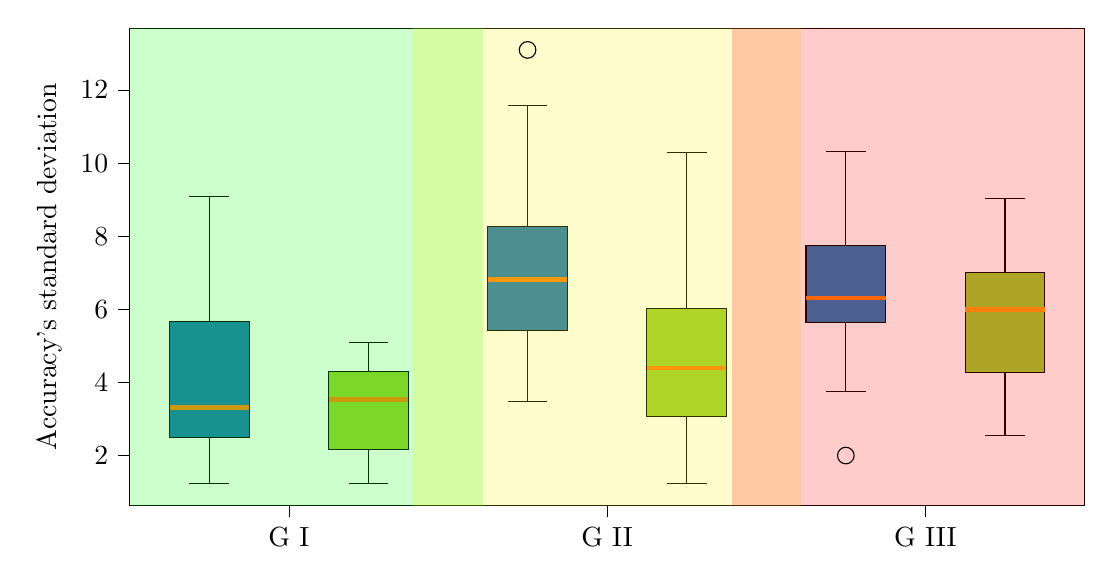
\begin{tikzpicture}

\definecolor{darkgray176}{RGB}{176,176,176}
\definecolor{darkorange25512714}{RGB}{255,127,14}
\definecolor{steelblue31119180}{RGB}{31,119,180}
\definecolor{yellowgreen}{RGB}{154, 205, 50}


\begin{axis}[
tick align=outside,
tick pos=left,
x grid style={darkgray176},
xmin=0.5, xmax=6.5,
xtick style={color=black},
y grid style={darkgray176},
ymin=0.63119207227573, ymax=13.6893536528247,
ytick style={color=black},
xtick={1.5,3.5,5.5},
xticklabels={
  G I,
  G II,
  G III
  },
  ylabel=Accuracy's standard deviation,
% only scale the axis, not the axis including the ticks and labels
scale only axis=true,
% set `width' and `height' to the desired values
width=\textwidth,
height=0.5\textwidth,
]
\path [draw=black, fill=steelblue31119180]
(axis cs:0.75,2.49949974978979)
--(axis cs:1.25,2.49949974978979)
--(axis cs:1.25,5.66066665775428)
--(axis cs:0.75,5.66066665775428)
--(axis cs:0.75,2.49949974978979)
--cycle;
\addplot [black]
table {%
1 2.49949974978979
1 1.22474487139159
};
\addplot [black]
table {%
1 5.66066665775428
1 9.08295106229247
};
\addplot [black]
table {%
0.875 1.22474487139159
1.125 1.22474487139159
};
\addplot [black]
table {%
0.875 9.08295106229247
1.125 9.08295106229247
};
\path [draw=black, fill=yellowgreen]
(axis cs:1.75,2.15987580880501)
--(axis cs:2.25,2.15987580880501)
--(axis cs:2.25,4.30116263352131)
--(axis cs:1.75,4.30116263352131)
--(axis cs:1.75,2.15987580880501)
--cycle;
\addplot [black]
table {%
2 2.15987580880501
2 1.22474487139159
};
\addplot [black]
table {%
2 4.30116263352131
2 5.09901951359278
};
\addplot [black]
table {%
1.875 1.22474487139159
2.125 1.22474487139159
};
\addplot [black]
table {%
1.875 5.09901951359278
2.125 5.09901951359278
};
\path [draw=black, fill=steelblue31119180]
(axis cs:2.75,5.42326317199804)
--(axis cs:3.25,5.42326317199804)
--(axis cs:3.25,8.25390718177714)
--(axis cs:2.75,8.25390718177714)
--(axis cs:2.75,5.42326317199804)
--cycle;
\addplot [black]
table {%
3 5.42326317199804
3 3.47811794006424
};
\addplot [black]
table {%
3 8.25390718177714
3 11.5758369027902
};
\addplot [black]
table {%
2.875 3.47811794006424
3.125 3.47811794006424
};
\addplot [black]
table {%
2.875 11.5758369027902
3.125 11.5758369027902
};
\addplot [black, mark=o, mark size=3, mark options={solid,fill opacity=0}, only marks]
table {%
3 13.0958008537088
};
\path [draw=black, fill=yellowgreen]
(axis cs:3.75,3.06488888954423)
--(axis cs:4.25,3.06488888954423)
--(axis cs:4.25,6.01614384783645)
--(axis cs:3.75,6.01614384783645)
--(axis cs:3.75,3.06488888954423)
--cycle;
\addplot [black]
table {%
4 3.06488888954423
4 1.22474487139159
};
\addplot [black]
table {%
4 6.01614384783645
4 10.295630140987
};
\addplot [black]
table {%
3.875 1.22474487139159
4.125 1.22474487139159
};
\addplot [black]
table {%
3.875 10.295630140987
4.125 10.295630140987
};
\path [draw=black, fill=steelblue31119180]
(axis cs:4.75,5.64386885355947)
--(axis cs:5.25,5.64386885355947)
--(axis cs:5.25,7.74700461664885)
--(axis cs:4.75,7.74700461664885)
--(axis cs:4.75,5.64386885355947)
--cycle;
\addplot [black]
table {%
5 5.64386885355947
5 3.74165738677394
};
\addplot [black]
table {%
5 7.74700461664885
5 10.3198837202751
};
\addplot [black]
table {%
4.875 3.74165738677394
5.125 3.74165738677394
};
\addplot [black]
table {%
4.875 10.3198837202751
5.125 10.3198837202751
};
\addplot [black, mark=o, mark size=3, mark options={solid,fill opacity=0}, only marks]
table {%
5 2
};
\path [draw=black, fill=yellowgreen]
(axis cs:5.75,4.26917420765551)
--(axis cs:6.25,4.26917420765551)
--(axis cs:6.25,7.00910803772708)
--(axis cs:5.75,7.00910803772708)
--(axis cs:5.75,4.26917420765551)
--cycle;
\addplot [black]
table {%
6 4.26917420765551
6 2.54950975679639
};
\addplot [black]
table {%
6 7.00910803772708
6 9.02773504263389
};
\addplot [black]
table {%
5.875 2.54950975679639
6.125 2.54950975679639
};
\addplot [black]
table {%
5.875 9.02773504263389
6.125 9.02773504263389
};
\addplot [ultra thick, darkorange25512714]
table {%
0.75 3.3166247903554
1.25 3.3166247903554
};
\addplot [ultra thick, darkorange25512714]
table {%
1.75 3.53553390593274
2.25 3.53553390593274
};
\addplot [ultra thick, darkorange25512714]
table {%
2.75 6.81909084849293
3.25 6.81909084849293
};
\addplot [ultra thick, darkorange25512714]
table {%
3.75 4.40194986679287
4.25 4.40194986679287
};
\addplot [ultra thick, darkorange25512714]
table {%
4.75 6.30398053021414
5.25 6.30398053021414
};

\path [draw=green, opacity=0.2, line width=140pt]
(axis cs:1.5,0.1)
--(axis cs:1.5,14);

\path [draw=yellow, opacity=0.2, line width=140pt]
(axis cs:3.5,0.1)
--(axis cs:3.5,14);

\path [draw=red, opacity=0.2, line width=140pt]
(axis cs:5.5,0.1)
--(axis cs:5.5,14);

\addplot [ultra thick, darkorange25512714]
table {%
5.75 6
6.25 6
};
\end{axis}
\end{tikzpicture}}
\end{frame}


\begin{frame}{Functional connectivity analysis I}
    \centering
    \resizebox{0.7\linewidth}{!}{%% Creator: Inkscape 1.2.2 (b0a8486541, 2022-12-01), www.inkscape.org
%% PDF/EPS/PS + LaTeX output extension by Johan Engelen, 2010
%% Accompanies image file 'Figures/Objective_2/pvalue-matrix_2.pdf' (pdf, eps, ps)
%%
%% To include the image in your LaTeX document, write
%%   \input{<filename>.pdf_tex}
%%  instead of
%%   \includegraphics{<filename>.pdf}
%% To scale the image, write
%%   \def\svgwidth{<desired width>}
%%   \input{<filename>.pdf_tex}
%%  instead of
%%   \includegraphics[width=<desired width>]{<filename>.pdf}
%%
%% Images with a different path to the parent latex file can
%% be accessed with the `import' package (which may need to be
%% installed) using
%%   \usepackage{import}
%% in the preamble, and then including the image with
%%   \import{<path to file>}{<filename>.pdf_tex}
%% Alternatively, one can specify
%%   \graphicspath{{<path to file>/}}
%% 
%% For more information, please see info/svg-inkscape on CTAN:
%%   http://tug.ctan.org/tex-archive/info/svg-inkscape
%%
\begingroup%
  \makeatletter%
  \providecommand\color[2][]{%
    \errmessage{(Inkscape) Color is used for the text in Inkscape, but the package 'color.sty' is not loaded}%
    \renewcommand\color[2][]{}%
  }%
  \providecommand\transparent[1]{%
    \errmessage{(Inkscape) Transparency is used (non-zero) for the text in Inkscape, but the package 'transparent.sty' is not loaded}%
    \renewcommand\transparent[1]{}%
  }%
  \providecommand\rotatebox[2]{#2}%
  \newcommand*\fsize{\dimexpr\f@size pt\relax}%
  \newcommand*\lineheight[1]{\fontsize{\fsize}{#1\fsize}\selectfont}%
  \ifx\svgwidth\undefined%
    \setlength{\unitlength}{578.92927515bp}%
    \ifx\svgscale\undefined%
      \relax%
    \else%
      \setlength{\unitlength}{\unitlength * \real{\svgscale}}%
    \fi%
  \else%
    \setlength{\unitlength}{\svgwidth}%
  \fi%
  \global\let\svgwidth\undefined%
  \global\let\svgscale\undefined%
  \makeatother%
  \begin{picture}(1,0.83623286)%
    \lineheight{1}%
    \setlength\tabcolsep{0pt}%
    \put(0,0){\includegraphics[width=\unitlength,page=1]{Figures/Objective_2/pvalue-matrix_2.pdf}}%
    \put(0.90737781,0.7925477){\color[rgb]{0,0,0}\makebox(0,0)[lt]{\lineheight{1.25}\smash{\begin{tabular}[t]{l}G.III\end{tabular}}}}%
    \put(0,0){\includegraphics[width=\unitlength,page=2]{Figures/Objective_2/pvalue-matrix_2.pdf}}%
    \put(0.90737781,0.75451951){\color[rgb]{0,0,0}\makebox(0,0)[lt]{\lineheight{1.25}\smash{\begin{tabular}[t]{l}G.II\end{tabular}}}}%
    \put(0,0){\includegraphics[width=\unitlength,page=3]{Figures/Objective_2/pvalue-matrix_2.pdf}}%
    \put(0.90737781,0.71649134){\color[rgb]{0,0,0}\makebox(0,0)[lt]{\lineheight{1.25}\smash{\begin{tabular}[t]{l}G.I\end{tabular}}}}%
    \put(0,0){\includegraphics[width=\unitlength,page=4]{Figures/Objective_2/pvalue-matrix_2.pdf}}%
    \put(-0.00115551,0.00028681){\color[rgb]{0,0,0}\makebox(0,0)[lt]{\lineheight{1.25}\smash{\begin{tabular}[t]{l}0.00\end{tabular}}}}%
    \put(0,0){\includegraphics[width=\unitlength,page=5]{Figures/Objective_2/pvalue-matrix_2.pdf}}%
    \put(0.0470369,0.00028681){\color[rgb]{0,0,0}\makebox(0,0)[lt]{\lineheight{1.25}\smash{\begin{tabular}[t]{l}0.05\end{tabular}}}}%
    \put(0,0){\includegraphics[width=\unitlength,page=6]{Figures/Objective_2/pvalue-matrix_2.pdf}}%
    \put(0.09522932,0.00028681){\color[rgb]{0,0,0}\makebox(0,0)[lt]{\lineheight{1.25}\smash{\begin{tabular}[t]{l}0.10\end{tabular}}}}%
    \put(0,0){\includegraphics[width=\unitlength,page=7]{Figures/Objective_2/pvalue-matrix_2.pdf}}%
    \put(0.19161414,0.00028681){\color[rgb]{0,0,0}\makebox(0,0)[lt]{\lineheight{1.25}\smash{\begin{tabular}[t]{l}0.20\end{tabular}}}}%
    \put(0,0){\includegraphics[width=\unitlength,page=8]{Figures/Objective_2/pvalue-matrix_2.pdf}}%
    \put(0.28799897,0.00028681){\color[rgb]{0,0,0}\makebox(0,0)[lt]{\lineheight{1.25}\smash{\begin{tabular}[t]{l}0.30\end{tabular}}}}%
    \put(0,0){\includegraphics[width=\unitlength,page=9]{Figures/Objective_2/pvalue-matrix_2.pdf}}%
    \put(0.38438379,0.00028681){\color[rgb]{0,0,0}\makebox(0,0)[lt]{\lineheight{1.25}\smash{\begin{tabular}[t]{l}0.40\end{tabular}}}}%
    \put(0,0){\includegraphics[width=\unitlength,page=10]{Figures/Objective_2/pvalue-matrix_2.pdf}}%
    \put(0.48076862,0.00028681){\color[rgb]{0,0,0}\makebox(0,0)[lt]{\lineheight{1.25}\smash{\begin{tabular}[t]{l}0.50\end{tabular}}}}%
    \put(0,0){\includegraphics[width=\unitlength,page=11]{Figures/Objective_2/pvalue-matrix_2.pdf}}%
    \put(0.57715344,0.00028681){\color[rgb]{0,0,0}\makebox(0,0)[lt]{\lineheight{1.25}\smash{\begin{tabular}[t]{l}0.60\end{tabular}}}}%
    \put(0,0){\includegraphics[width=\unitlength,page=12]{Figures/Objective_2/pvalue-matrix_2.pdf}}%
    \put(0.67353827,0.00028681){\color[rgb]{0,0,0}\makebox(0,0)[lt]{\lineheight{1.25}\smash{\begin{tabular}[t]{l}0.70\end{tabular}}}}%
    \put(0,0){\includegraphics[width=\unitlength,page=13]{Figures/Objective_2/pvalue-matrix_2.pdf}}%
    \put(0.7699231,0.00028681){\color[rgb]{0,0,0}\makebox(0,0)[lt]{\lineheight{1.25}\smash{\begin{tabular}[t]{l}0.80\end{tabular}}}}%
    \put(0,0){\includegraphics[width=\unitlength,page=14]{Figures/Objective_2/pvalue-matrix_2.pdf}}%
    \put(0.86630792,0.00028681){\color[rgb]{0,0,0}\makebox(0,0)[lt]{\lineheight{1.25}\smash{\begin{tabular}[t]{l}0.90\end{tabular}}}}%
    \put(0,0){\includegraphics[width=\unitlength,page=15]{Figures/Objective_2/pvalue-matrix_2.pdf}}%
    \put(0.96269275,0.00028681){\color[rgb]{0,0,0}\makebox(0,0)[lt]{\lineheight{1.25}\smash{\begin{tabular}[t]{l}1.00\end{tabular}}}}%
    \put(0,0){\includegraphics[width=\unitlength,page=16]{Figures/Objective_2/pvalue-matrix_2.pdf}}%
  \end{picture}%
\endgroup%
}
\end{frame}

\begin{frame}{Functional connectivity analysis II}
    \centering
    \resizebox{0.7\linewidth}{!}{% This file was created with tikzplotlib v0.10.1.
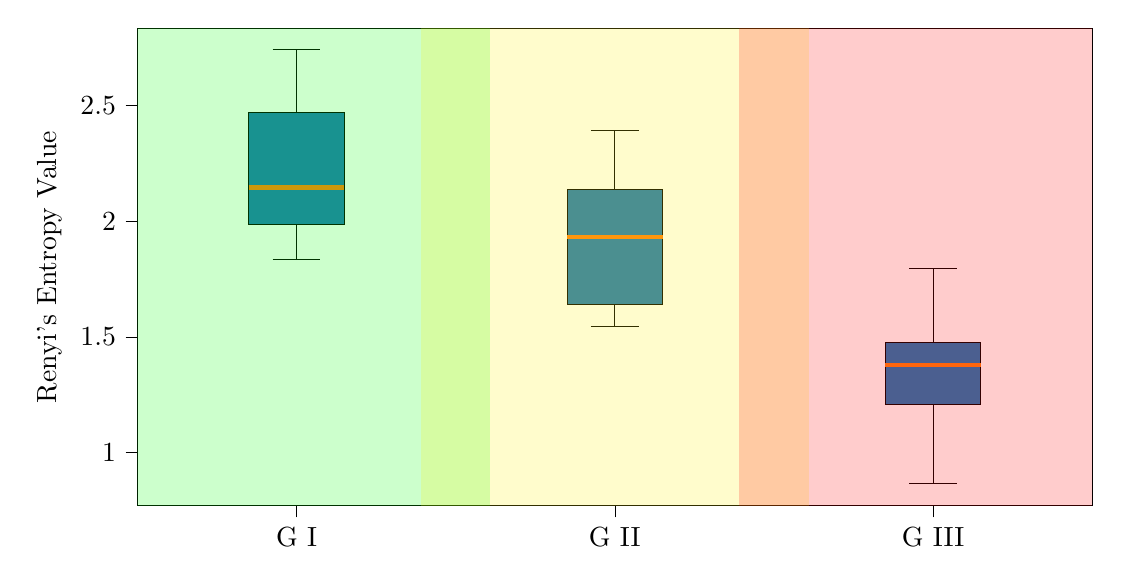
\begin{tikzpicture}

\definecolor{darkgray176}{RGB}{176,176,176}
\definecolor{darkorange25512714}{RGB}{255,127,14}
\definecolor{steelblue31119180}{RGB}{31,119,180}

\begin{axis}[
tick align=outside,
tick pos=left,
x grid style={darkgray176},
xmin=0.5, xmax=3.5,
xtick style={color=black},
y grid style={darkgray176},
ylabel={Renyi's Entropy Value},
ymin=0.770107169384725, ymax=2.83550014961814,
ytick style={color=black},
xtick={1,2,3},
xticklabels={
  G I,
  G II,
  G III
  },
% only scale the axis, not the axis including the ticks and labels
scale only axis=true,
% set `width' and `height' to the desired values
width=\textwidth,
height=0.5\textwidth,
]
\path [draw=black, fill=steelblue31119180]
(axis cs:0.85,1.98710265444379)
--(axis cs:1.15,1.98710265444379)
--(axis cs:1.15,2.4692055467728)
--(axis cs:0.85,2.4692055467728)
--(axis cs:0.85,1.98710265444379)
--cycle;
\addplot [black]
table {%
1 1.98710265444379
1 1.83340962365363
};
\addplot [black]
table {%
1 2.4692055467728
1 2.74161865051662
};
\addplot [black]
table {%
0.925 1.83340962365363
1.075 1.83340962365363
};
\addplot [black]
table {%
0.925 2.74161865051662
1.075 2.74161865051662
};
\path [draw=black, fill=steelblue31119180]
(axis cs:1.85,1.64091629667123)
--(axis cs:2.15,1.64091629667123)
--(axis cs:2.15,2.13763307187243)
--(axis cs:1.85,2.13763307187243)
--(axis cs:1.85,1.64091629667123)
--cycle;
\addplot [black]
table {%
2 1.64091629667123
2 1.54325014822209
};
\addplot [black]
table {%
2 2.13763307187243
2 2.39465148485741
};
\addplot [black]
table {%
1.925 1.54325014822209
2.075 1.54325014822209
};
\addplot [black]
table {%
1.925 2.39465148485741
2.075 2.39465148485741
};
\path [draw=black, fill=steelblue31119180]
(axis cs:2.85,1.20701646656938)
--(axis cs:3.15,1.20701646656938)
--(axis cs:3.15,1.47736138105042)
--(axis cs:2.85,1.47736138105042)
--(axis cs:2.85,1.20701646656938)
--cycle;
\addplot [black]
table {%
3 1.20701646656938
3 0.863988668486244
};
\addplot [black]
table {%
3 1.47736138105042
3 1.7973903501163
};
\addplot [black]
table {%
2.925 0.863988668486244
3.075 0.863988668486244
};
\addplot [black]
table {%
2.925 1.7973903501163
3.075 1.7973903501163
};
\addplot [ultra thick, darkorange25512714]
table {%
0.85 2.14641792100428
1.15 2.14641792100428
};
\addplot [ultra thick, darkorange25512714]
table {%
1.85 1.93151078195408
2.15 1.93151078195408
};
\addplot [ultra thick, darkorange25512714]
table {%
2.85 1.3773748804191
3.15 1.3773748804191
};

\path [draw=green, opacity=0.2, line width=140pt]
(axis cs:1,0.1)
--(axis cs:1,3);

\path [draw=yellow, opacity=0.2, line width=140pt]
(axis cs:2,0.1)
--(axis cs:2,3);

\path [draw=red, opacity=0.2, line width=140pt]
(axis cs:3,0.1)
--(axis cs:3,3);


\end{axis}

\end{tikzpicture}
}
\end{frame}


\begin{frame}{Functional connectivity analysis III}
    \begin{figure}
        \centering
       \begin{subfigure}[b]{.13\linewidth}
           \centering
           \resizebox{1\linewidth}{!}{%% Creator: Inkscape 1.2.2 (b0a8486541, 2022-12-01), www.inkscape.org
%% PDF/EPS/PS + LaTeX output extension by Johan Engelen, 2010
%% Accompanies image file 'goood.pdf' (pdf, eps, ps)
%%
%% To include the image in your LaTeX document, write
%%   \input{<filename>.pdf_tex}
%%  instead of
%%   \includegraphics{<filename>.pdf}
%% To scale the image, write
%%   \def\svgwidth{<desired width>}
%%   \input{<filename>.pdf_tex}
%%  instead of
%%   \includegraphics[width=<desired width>]{<filename>.pdf}
%%
%% Images with a different path to the parent latex file can
%% be accessed with the `import' package (which may need to be
%% installed) using
%%   \usepackage{import}
%% in the preamble, and then including the image with
%%   \import{<path to file>}{<filename>.pdf_tex}
%% Alternatively, one can specify
%%   \graphicspath{{<path to file>/}}
%% 
%% For more information, please see info/svg-inkscape on CTAN:
%%   http://tug.ctan.org/tex-archive/info/svg-inkscape
%%
\begingroup%
  \makeatletter%
  \providecommand\color[2][]{%
    \errmessage{(Inkscape) Color is used for the text in Inkscape, but the package 'color.sty' is not loaded}%
    \renewcommand\color[2][]{}%
  }%
  \providecommand\transparent[1]{%
    \errmessage{(Inkscape) Transparency is used (non-zero) for the text in Inkscape, but the package 'transparent.sty' is not loaded}%
    \renewcommand\transparent[1]{}%
  }%
  \providecommand\rotatebox[2]{#2}%
  \newcommand*\fsize{\dimexpr\f@size pt\relax}%
  \newcommand*\lineheight[1]{\fontsize{\fsize}{#1\fsize}\selectfont}%
  \ifx\svgwidth\undefined%
    \setlength{\unitlength}{719.99997449bp}%
    \ifx\svgscale\undefined%
      \relax%
    \else%
      \setlength{\unitlength}{\unitlength * \real{\svgscale}}%
    \fi%
  \else%
    \setlength{\unitlength}{\svgwidth}%
  \fi%
  \global\let\svgwidth\undefined%
  \global\let\svgscale\undefined%
  \makeatother%
  \begin{picture}(1,1.00000004)%
    \lineheight{1}%
    \setlength\tabcolsep{0pt}%
    \put(0,0){\includegraphics[width=\unitlength,page=1]{Figures/Objective_2/circonnecitvity_good_2.pdf}}%
    \put(0.46180678,0.92326249){\color[rgb]{0,0,0}\rotatebox{-1.25000007}{\makebox(0,0)[lt]{\lineheight{1.25}\smash{\begin{tabular}[t]{l} \LARGE Frontal\end{tabular}}}}}%
    \put(0.66112171,0.90027214){\color[rgb]{0,0,0}\rotatebox{-33.7500015}{\makebox(0,0)[lt]{\lineheight{1.25}\smash{\begin{tabular}[t]{l} \LARGE Frontal Right\end{tabular}}}}}%
    \put(0.91543541,0.61899459){\color[rgb]{0,0,0}\rotatebox{-86.25000021}{\makebox(0,0)[lt]{\lineheight{1.25}\smash{\begin{tabular}[t]{l} \LARGE Central Right\end{tabular}}}}}%
    \put(0.69412406,0.09460069){\color[rgb]{0,0,0}\rotatebox{38.75000159}{\makebox(0,0)[lt]{\lineheight{1.25}\smash{\begin{tabular}[t]{l} \LARGE Posterior Right\end{tabular}}}}}%
    \put(0.42910617,0.06377129){\color[rgb]{0,0,0}\rotatebox{-1.25000007}{\makebox(0,0)[lt]{\lineheight{1.25}\smash{\begin{tabular}[t]{l} \LARGE Posterior\end{tabular}}}}}%
    \put(0.14234136,0.23152432){\color[rgb]{0,0,0}\rotatebox{-41.25000161}{\makebox(0,0)[lt]{\lineheight{1.25}\smash{\begin{tabular}[t]{l} \LARGE Posterior Left\end{tabular}}}}}%
    \put(0.07135272,0.46536155){\color[rgb]{0,0,0}\rotatebox{83.75000035}{\makebox(0,0)[lt]{\lineheight{1.25}\smash{\begin{tabular}[t]{l} \LARGE Central Left\end{tabular}}}}}%
    \put(0.21427494,0.82062027){\color[rgb]{0,0,0}\rotatebox{31.25000144}{\makebox(0,0)[lt]{\lineheight{1.25}\smash{\begin{tabular}[t]{l} \LARGE Frontal Left\end{tabular}}}}}%
    \put(0.43605392,0.8625217){\color[rgb]{0,0,0}\rotatebox{6.25000035}{\makebox(0,0)[lt]{\lineheight{1.25}\smash{\begin{tabular}[t]{l} \LARGE Fpz\end{tabular}}}}}%
    \put(0.46720968,0.86670054){\color[rgb]{0,0,0}\rotatebox{1.25000007}{\makebox(0,0)[lt]{\lineheight{1.25}\smash{\begin{tabular}[t]{l} \LARGE AFz\end{tabular}}}}}%
    \put(0.50877937,0.86754133){\color[rgb]{0,0,0}\rotatebox{-3.75000021}{\makebox(0,0)[lt]{\lineheight{1.25}\smash{\begin{tabular}[t]{l} \LARGE Fz\end{tabular}}}}}%
    \put(0.53119168,0.86685322){\color[rgb]{0,0,0}\rotatebox{-8.75000049}{\makebox(0,0)[lt]{\lineheight{1.25}\smash{\begin{tabular}[t]{l} \LARGE FCz\end{tabular}}}}}%
    \put(0.59379441,0.85607626){\color[rgb]{0,0,0}\rotatebox{-18.75000099}{\makebox(0,0)[lt]{\lineheight{1.25}\smash{\begin{tabular}[t]{l} \LARGE Fp2\end{tabular}}}}}%
    \put(0.6238459,0.84682192){\color[rgb]{0,0,0}\rotatebox{-23.7500012}{\makebox(0,0)[lt]{\lineheight{1.25}\smash{\begin{tabular}[t]{l} \LARGE AF4\end{tabular}}}}}%
    \put(0.65360213,0.83470826){\color[rgb]{0,0,0}\rotatebox{-28.75000137}{\makebox(0,0)[lt]{\lineheight{1.25}\smash{\begin{tabular}[t]{l} \LARGE AF8\end{tabular}}}}}%
    \put(0.69009268,0.8147665){\color[rgb]{0,0,0}\rotatebox{-33.7500015}{\makebox(0,0)[lt]{\lineheight{1.25}\smash{\begin{tabular}[t]{l} \LARGE F2\end{tabular}}}}}%
    \put(0.71680301,0.79700102){\color[rgb]{0,0,0}\rotatebox{-38.75000159}{\makebox(0,0)[lt]{\lineheight{1.25}\smash{\begin{tabular}[t]{l} \LARGE F4\end{tabular}}}}}%
    \put(0.74186335,0.77697521){\color[rgb]{0,0,0}\rotatebox{-43.75000162}{\makebox(0,0)[lt]{\lineheight{1.25}\smash{\begin{tabular}[t]{l} \LARGE F6\end{tabular}}}}}%
    \put(0.76508297,0.75484145){\color[rgb]{0,0,0}\rotatebox{-48.75000161}{\makebox(0,0)[lt]{\lineheight{1.25}\smash{\begin{tabular}[t]{l} \LARGE F8\end{tabular}}}}}%
    \put(0.80027614,0.71323175){\color[rgb]{0,0,0}\rotatebox{-58.75000144}{\makebox(0,0)[lt]{\lineheight{1.25}\smash{\begin{tabular}[t]{l} \LARGE FC2\end{tabular}}}}}%
    \put(0.81771786,0.68624956){\color[rgb]{0,0,0}\rotatebox{-63.75000129}{\makebox(0,0)[lt]{\lineheight{1.25}\smash{\begin{tabular}[t]{l} \LARGE FC4\end{tabular}}}}}%
    \put(0.83274157,0.65784988){\color[rgb]{0,0,0}\rotatebox{-68.7500011}{\makebox(0,0)[lt]{\lineheight{1.25}\smash{\begin{tabular}[t]{l} \LARGE FC6\end{tabular}}}}}%
    \put(0.84564585,0.62683212){\color[rgb]{0,0,0}\rotatebox{-73.75000087}{\makebox(0,0)[lt]{\lineheight{1.25}\smash{\begin{tabular}[t]{l} \LARGE FT8\end{tabular}}}}}%
    \put(0.85665482,0.58983915){\color[rgb]{0,0,0}\rotatebox{-78.75000062}{\makebox(0,0)[lt]{\lineheight{1.25}\smash{\begin{tabular}[t]{l} \LARGE C2\end{tabular}}}}}%
    \put(0.86312764,0.55841276){\color[rgb]{0,0,0}\rotatebox{-83.75000035}{\makebox(0,0)[lt]{\lineheight{1.25}\smash{\begin{tabular}[t]{l} \LARGE C4\end{tabular}}}}}%
    \put(0.86683684,0.52654182){\color[rgb]{0,0,0}\rotatebox{-88.75000007}{\makebox(0,0)[lt]{\lineheight{1.25}\smash{\begin{tabular}[t]{l} \LARGE C6\end{tabular}}}}}%
    \put(0.8676747,0.49325621){\color[rgb]{0,0,0}\rotatebox{-93.74999979}{\makebox(0,0)[lt]{\lineheight{1.25}\smash{\begin{tabular}[t]{l} \LARGE T8\end{tabular}}}}}%
    \put(0.867147,0.47071729){\color[rgb]{0,0,0}\rotatebox{-98.74999951}{\makebox(0,0)[lt]{\lineheight{1.25}\smash{\begin{tabular}[t]{l} \LARGE CP2\end{tabular}}}}}%
    \put(0.86319773,0.43882974){\color[rgb]{0,0,0}\rotatebox{-103.74999925}{\makebox(0,0)[lt]{\lineheight{1.25}\smash{\begin{tabular}[t]{l} \LARGE CP4\end{tabular}}}}}%
    \put(0.85648432,0.40740775){\color[rgb]{0,0,0}\rotatebox{-108.74999901}{\makebox(0,0)[lt]{\lineheight{1.25}\smash{\begin{tabular}[t]{l} \LARGE CP6\end{tabular}}}}}%
    \put(0.84656839,0.37557808){\color[rgb]{0,0,0}\rotatebox{-113.7499988}{\makebox(0,0)[lt]{\lineheight{1.25}\smash{\begin{tabular}[t]{l} \LARGE TP8\end{tabular}}}}}%
    \put(0.81498344,0.31023213){\color[rgb]{0,0,0}\rotatebox{-123.7499985}{\makebox(0,0)[lt]{\lineheight{1.25}\smash{\begin{tabular}[t]{l} \LARGE P2\end{tabular}}}}}%
    \put(0.79724547,0.28350163){\color[rgb]{0,0,0}\rotatebox{-128.74999841}{\makebox(0,0)[lt]{\lineheight{1.25}\smash{\begin{tabular}[t]{l} \LARGE P4\end{tabular}}}}}%
    \put(0.77724528,0.25841882){\color[rgb]{0,0,0}\rotatebox{-133.74999838}{\makebox(0,0)[lt]{\lineheight{1.25}\smash{\begin{tabular}[t]{l} \LARGE P6\end{tabular}}}}}%
    \put(0.7551351,0.23517459){\color[rgb]{0,0,0}\rotatebox{-138.74999839}{\makebox(0,0)[lt]{\lineheight{1.25}\smash{\begin{tabular}[t]{l} \LARGE P8\end{tabular}}}}}%
    \put(0.73820608,0.21916857){\color[rgb]{0,0,0}\rotatebox{-143.74999845}{\makebox(0,0)[lt]{\lineheight{1.25}\smash{\begin{tabular}[t]{l} \LARGE P10\end{tabular}}}}}%
    \put(0.71462318,0.20056822){\color[rgb]{0,0,0}\rotatebox{-148.74999856}{\makebox(0,0)[lt]{\lineheight{1.25}\smash{\begin{tabular}[t]{l} \LARGE PO4\end{tabular}}}}}%
    \put(0.68770927,0.183002){\color[rgb]{0,0,0}\rotatebox{-153.74999871}{\makebox(0,0)[lt]{\lineheight{1.25}\smash{\begin{tabular}[t]{l} \LARGE PO8\end{tabular}}}}}%
    \put(0.65155961,0.16481229){\color[rgb]{0,0,0}\rotatebox{-158.7499989}{\makebox(0,0)[lt]{\lineheight{1.25}\smash{\begin{tabular}[t]{l} \LARGE O2\end{tabular}}}}}%
    \put(0.59654371,0.14467879){\color[rgb]{0,0,0}\rotatebox{-168.74999938}{\makebox(0,0)[lt]{\lineheight{1.25}\smash{\begin{tabular}[t]{l} \LARGE CPz\end{tabular}}}}}%
    \put(0.55556518,0.13656049){\color[rgb]{0,0,0}\rotatebox{-173.74999965}{\makebox(0,0)[lt]{\lineheight{1.25}\smash{\begin{tabular}[t]{l} \LARGE Pz\end{tabular}}}}}%
    \put(0.52500136,0.13312954){\color[rgb]{0,0,0}\rotatebox{-178.74999993}{\makebox(0,0)[lt]{\lineheight{1.25}\smash{\begin{tabular}[t]{l} \LARGE Cz\end{tabular}}}}}%
    \put(0.50252449,0.13171782){\color[rgb]{0,0,0}\rotatebox{176.24999979}{\makebox(0,0)[lt]{\lineheight{1.25}\smash{\begin{tabular}[t]{l} \LARGE POz\end{tabular}}}}}%
    \put(0.46213775,0.13417351){\color[rgb]{0,0,0}\rotatebox{171.24999951}{\makebox(0,0)[lt]{\lineheight{1.25}\smash{\begin{tabular}[t]{l} \LARGE Oz\end{tabular}}}}}%
    \put(0.42375791,0.14049031){\color[rgb]{0,0,0}\rotatebox{166.24999925}{\makebox(0,0)[lt]{\lineheight{1.25}\smash{\begin{tabular}[t]{l} \LARGE Iz\end{tabular}}}}}%
    \put(0.3678114,0.15684901){\color[rgb]{0,0,0}\rotatebox{156.2499988}{\makebox(0,0)[lt]{\lineheight{1.25}\smash{\begin{tabular}[t]{l} \LARGE P1\end{tabular}}}}}%
    \put(0.33840684,0.1696758){\color[rgb]{0,0,0}\rotatebox{151.24999863}{\makebox(0,0)[lt]{\lineheight{1.25}\smash{\begin{tabular}[t]{l} \LARGE P3\end{tabular}}}}}%
    \put(0.31023211,0.18501654){\color[rgb]{0,0,0}\rotatebox{146.2499985}{\makebox(0,0)[lt]{\lineheight{1.25}\smash{\begin{tabular}[t]{l} \LARGE P5\end{tabular}}}}}%
    \put(0.28350162,0.20275452){\color[rgb]{0,0,0}\rotatebox{141.24999841}{\makebox(0,0)[lt]{\lineheight{1.25}\smash{\begin{tabular}[t]{l} \LARGE P7\end{tabular}}}}}%
    \put(0.25841881,0.22275471){\color[rgb]{0,0,0}\rotatebox{136.24999838}{\makebox(0,0)[lt]{\lineheight{1.25}\smash{\begin{tabular}[t]{l} \LARGE P9\end{tabular}}}}}%
    \put(0.24238617,0.23664165){\color[rgb]{0,0,0}\rotatebox{131.24999839}{\makebox(0,0)[lt]{\lineheight{1.25}\smash{\begin{tabular}[t]{l} \LARGE PO3\end{tabular}}}}}%
    \put(0.22041328,0.26009634){\color[rgb]{0,0,0}\rotatebox{126.24999845}{\makebox(0,0)[lt]{\lineheight{1.25}\smash{\begin{tabular}[t]{l} \LARGE PO7\end{tabular}}}}}%
    \put(0.19622259,0.29253821){\color[rgb]{0,0,0}\rotatebox{121.24999856}{\makebox(0,0)[lt]{\lineheight{1.25}\smash{\begin{tabular}[t]{l} \LARGE O1\end{tabular}}}}}%
    \put(0.16725842,0.34215017){\color[rgb]{0,0,0}\rotatebox{111.2499989}{\makebox(0,0)[lt]{\lineheight{1.25}\smash{\begin{tabular}[t]{l} \LARGE FC1\end{tabular}}}}}%
    \put(0.15476708,0.37175117){\color[rgb]{0,0,0}\rotatebox{106.24999913}{\makebox(0,0)[lt]{\lineheight{1.25}\smash{\begin{tabular}[t]{l} \LARGE FC3\end{tabular}}}}}%
    \put(0.14490317,0.40232822){\color[rgb]{0,0,0}\rotatebox{101.24999938}{\makebox(0,0)[lt]{\lineheight{1.25}\smash{\begin{tabular}[t]{l} \LARGE FC5\end{tabular}}}}}%
    \put(0.13758111,0.43511555){\color[rgb]{0,0,0}\rotatebox{96.24999965}{\makebox(0,0)[lt]{\lineheight{1.25}\smash{\begin{tabular}[t]{l} \LARGE FT7\end{tabular}}}}}%
    \put(0.13316316,0.47345821){\color[rgb]{0,0,0}\rotatebox{91.24999993}{\makebox(0,0)[lt]{\lineheight{1.25}\smash{\begin{tabular}[t]{l} \LARGE C1\end{tabular}}}}}%
    \put(0.1322458,0.50553114){\color[rgb]{0,0,0}\rotatebox{86.25000021}{\makebox(0,0)[lt]{\lineheight{1.25}\smash{\begin{tabular}[t]{l} \LARGE C3\end{tabular}}}}}%
    \put(0.13412729,0.537562){\color[rgb]{0,0,0}\rotatebox{81.25000049}{\makebox(0,0)[lt]{\lineheight{1.25}\smash{\begin{tabular}[t]{l} \LARGE C5\end{tabular}}}}}%
    \put(0.13908213,0.57048742){\color[rgb]{0,0,0}\rotatebox{76.25000075}{\makebox(0,0)[lt]{\lineheight{1.25}\smash{\begin{tabular}[t]{l} \LARGE T7\end{tabular}}}}}%
    \put(0.14351567,0.5925923){\color[rgb]{0,0,0}\rotatebox{71.25000099}{\makebox(0,0)[lt]{\lineheight{1.25}\smash{\begin{tabular}[t]{l} \LARGE CP1\end{tabular}}}}}%
    \put(0.15294215,0.62330961){\color[rgb]{0,0,0}\rotatebox{66.2500012}{\makebox(0,0)[lt]{\lineheight{1.25}\smash{\begin{tabular}[t]{l} \LARGE CP3\end{tabular}}}}}%
    \put(0.16500994,0.65308847){\color[rgb]{0,0,0}\rotatebox{61.25000137}{\makebox(0,0)[lt]{\lineheight{1.25}\smash{\begin{tabular}[t]{l} \LARGE CP5\end{tabular}}}}}%
    \put(0.18030239,0.68271269){\color[rgb]{0,0,0}\rotatebox{56.2500015}{\makebox(0,0)[lt]{\lineheight{1.25}\smash{\begin{tabular}[t]{l} \LARGE TP7\end{tabular}}}}}%
    \put(0.21692456,0.73549098){\color[rgb]{0,0,0}\rotatebox{46.25000162}{\makebox(0,0)[lt]{\lineheight{1.25}\smash{\begin{tabular}[t]{l} \LARGE Fp1\end{tabular}}}}}%
    \put(0.23801218,0.75881579){\color[rgb]{0,0,0}\rotatebox{41.25000161}{\makebox(0,0)[lt]{\lineheight{1.25}\smash{\begin{tabular}[t]{l} \LARGE AF3\end{tabular}}}}}%
    \put(0.2615664,0.78066466){\color[rgb]{0,0,0}\rotatebox{36.25000155}{\makebox(0,0)[lt]{\lineheight{1.25}\smash{\begin{tabular}[t]{l} \LARGE AF7\end{tabular}}}}}%
    \put(0.29506136,0.80530855){\color[rgb]{0,0,0}\rotatebox{31.25000144}{\makebox(0,0)[lt]{\lineheight{1.25}\smash{\begin{tabular}[t]{l} \LARGE F1\end{tabular}}}}}%
    \put(0.3224506,0.82200836){\color[rgb]{0,0,0}\rotatebox{26.25000129}{\makebox(0,0)[lt]{\lineheight{1.25}\smash{\begin{tabular}[t]{l} \LARGE F3\end{tabular}}}}}%
    \put(0.3511911,0.83625747){\color[rgb]{0,0,0}\rotatebox{21.2500011}{\makebox(0,0)[lt]{\lineheight{1.25}\smash{\begin{tabular}[t]{l} \LARGE F5\end{tabular}}}}}%
    \put(0.38106413,0.84794743){\color[rgb]{0,0,0}\rotatebox{16.25000087}{\makebox(0,0)[lt]{\lineheight{1.25}\smash{\begin{tabular}[t]{l} \LARGE F7\end{tabular}}}}}%
  \end{picture}%
\endgroup%
}
       \end{subfigure}
       ~
       \begin{subfigure}[b]{.13\linewidth}
           \centering 	\resizebox{1\linewidth}{!}{\input{figures/circonnecitvity_medium_2}}	
       \end{subfigure}
       ~
       \begin{subfigure}[b]{.13\linewidth}
           \centering
           \resizebox{1\linewidth}{!}{%% Creator: Inkscape 1.2.2 (b0a8486541, 2022-12-01), www.inkscape.org
%% PDF/EPS/PS + LaTeX output extension by Johan Engelen, 2010
%% Accompanies image file 'circonnecitvity_bad.pdf' (pdf, eps, ps)
%%
%% To include the image in your LaTeX document, write
%%   \input{<filename>.pdf_tex}
%%  instead of
%%   \includegraphics{<filename>.pdf}
%% To scale the image, write
%%   \def\svgwidth{<desired width>}
%%   \input{<filename>.pdf_tex}
%%  instead of
%%   \includegraphics[width=<desired width>]{<filename>.pdf}
%%
%% Images with a different path to the parent latex file can
%% be accessed with the `import' package (which may need to be
%% installed) using
%%   \usepackage{import}
%% in the preamble, and then including the image with
%%   \import{<path to file>}{<filename>.pdf_tex}
%% Alternatively, one can specify
%%   \graphicspath{{<path to file>/}}
%% 
%% For more information, please see info/svg-inkscape on CTAN:
%%   http://tug.ctan.org/tex-archive/info/svg-inkscape
%%
\begingroup%
  \makeatletter%
  \providecommand\color[2][]{%
    \errmessage{(Inkscape) Color is used for the text in Inkscape, but the package 'color.sty' is not loaded}%
    \renewcommand\color[2][]{}%
  }%
  \providecommand\transparent[1]{%
    \errmessage{(Inkscape) Transparency is used (non-zero) for the text in Inkscape, but the package 'transparent.sty' is not loaded}%
    \renewcommand\transparent[1]{}%
  }%
  \providecommand\rotatebox[2]{#2}%
  \newcommand*\fsize{\dimexpr\f@size pt\relax}%
  \newcommand*\lineheight[1]{\fontsize{\fsize}{#1\fsize}\selectfont}%
  \ifx\svgwidth\undefined%
    \setlength{\unitlength}{719.9999915bp}%
    \ifx\svgscale\undefined%
      \relax%
    \else%
      \setlength{\unitlength}{\unitlength * \real{\svgscale}}%
    \fi%
  \else%
    \setlength{\unitlength}{\svgwidth}%
  \fi%
  \global\let\svgwidth\undefined%
  \global\let\svgscale\undefined%
  \makeatother%
  \begin{picture}(1,1.00000002)%
    \lineheight{1}%
    \setlength\tabcolsep{0pt}%
    \put(0,0){\includegraphics[width=\unitlength,page=1]{Figures/Objective_2/circonnecitvity_bad_2.pdf}}%
    \put(0.46180677,0.92326247){\color[rgb]{0,0,0}\rotatebox{-1.25000007}{\makebox(0,0)[lt]{\lineheight{1.25}\smash{\begin{tabular}[t]{l} \LARGE Frontal\end{tabular}}}}}%
    \put(0.6611217,0.90027212){\color[rgb]{0,0,0}\rotatebox{-33.7500015}{\makebox(0,0)[lt]{\lineheight{1.25}\smash{\begin{tabular}[t]{l} \LARGE Frontal Right\end{tabular}}}}}%
    \put(0.91543539,0.61899458){\color[rgb]{0,0,0}\rotatebox{-86.25000021}{\makebox(0,0)[lt]{\lineheight{1.25}\smash{\begin{tabular}[t]{l} \LARGE Central Right\end{tabular}}}}}%
    \put(0.69412404,0.09460069){\color[rgb]{0,0,0}\rotatebox{38.75000159}{\makebox(0,0)[lt]{\lineheight{1.25}\smash{\begin{tabular}[t]{l} \LARGE Posterior Right\end{tabular}}}}}%
    \put(0.42910616,0.06377129){\color[rgb]{0,0,0}\rotatebox{-1.25000007}{\makebox(0,0)[lt]{\lineheight{1.25}\smash{\begin{tabular}[t]{l} \LARGE Posterior\end{tabular}}}}}%
    \put(0.14234135,0.23152431){\color[rgb]{0,0,0}\rotatebox{-41.25000161}{\makebox(0,0)[lt]{\lineheight{1.25}\smash{\begin{tabular}[t]{l} \LARGE Posterior Left\end{tabular}}}}}%
    \put(0.07135272,0.46536153){\color[rgb]{0,0,0}\rotatebox{83.75000035}{\makebox(0,0)[lt]{\lineheight{1.25}\smash{\begin{tabular}[t]{l} \LARGE Central Left\end{tabular}}}}}%
    \put(0.21427494,0.82062025){\color[rgb]{0,0,0}\rotatebox{31.25000144}{\makebox(0,0)[lt]{\lineheight{1.25}\smash{\begin{tabular}[t]{l} \LARGE Frontal Left\end{tabular}}}}}%
    \put(0.43605391,0.86252168){\color[rgb]{0,0,0}\rotatebox{6.25000035}{\makebox(0,0)[lt]{\lineheight{1.25}\smash{\begin{tabular}[t]{l} \LARGE Fpz\end{tabular}}}}}%
    \put(0.46720967,0.86670052){\color[rgb]{0,0,0}\rotatebox{1.25000007}{\makebox(0,0)[lt]{\lineheight{1.25}\smash{\begin{tabular}[t]{l} \LARGE AFz\end{tabular}}}}}%
    \put(0.50877935,0.86754131){\color[rgb]{0,0,0}\rotatebox{-3.75000021}{\makebox(0,0)[lt]{\lineheight{1.25}\smash{\begin{tabular}[t]{l} \LARGE Fz\end{tabular}}}}}%
    \put(0.53119166,0.8668532){\color[rgb]{0,0,0}\rotatebox{-8.75000049}{\makebox(0,0)[lt]{\lineheight{1.25}\smash{\begin{tabular}[t]{l} \LARGE FCz\end{tabular}}}}}%
    \put(0.5937944,0.85607624){\color[rgb]{0,0,0}\rotatebox{-18.75000099}{\makebox(0,0)[lt]{\lineheight{1.25}\smash{\begin{tabular}[t]{l} \LARGE Fp2\end{tabular}}}}}%
    \put(0.62384588,0.8468219){\color[rgb]{0,0,0}\rotatebox{-23.7500012}{\makebox(0,0)[lt]{\lineheight{1.25}\smash{\begin{tabular}[t]{l} \LARGE AF4\end{tabular}}}}}%
    \put(0.65360212,0.83470824){\color[rgb]{0,0,0}\rotatebox{-28.75000137}{\makebox(0,0)[lt]{\lineheight{1.25}\smash{\begin{tabular}[t]{l} \LARGE AF8\end{tabular}}}}}%
    \put(0.69009266,0.81476648){\color[rgb]{0,0,0}\rotatebox{-33.7500015}{\makebox(0,0)[lt]{\lineheight{1.25}\smash{\begin{tabular}[t]{l} \LARGE F2\end{tabular}}}}}%
    \put(0.71680299,0.797001){\color[rgb]{0,0,0}\rotatebox{-38.75000159}{\makebox(0,0)[lt]{\lineheight{1.25}\smash{\begin{tabular}[t]{l} \LARGE F4\end{tabular}}}}}%
    \put(0.74186333,0.77697519){\color[rgb]{0,0,0}\rotatebox{-43.75000162}{\makebox(0,0)[lt]{\lineheight{1.25}\smash{\begin{tabular}[t]{l} \LARGE F6\end{tabular}}}}}%
    \put(0.76508295,0.75484144){\color[rgb]{0,0,0}\rotatebox{-48.75000161}{\makebox(0,0)[lt]{\lineheight{1.25}\smash{\begin{tabular}[t]{l} \LARGE F8\end{tabular}}}}}%
    \put(0.80027612,0.71323173){\color[rgb]{0,0,0}\rotatebox{-58.75000144}{\makebox(0,0)[lt]{\lineheight{1.25}\smash{\begin{tabular}[t]{l} \LARGE FC2\end{tabular}}}}}%
    \put(0.81771784,0.68624954){\color[rgb]{0,0,0}\rotatebox{-63.75000129}{\makebox(0,0)[lt]{\lineheight{1.25}\smash{\begin{tabular}[t]{l} \LARGE FC4\end{tabular}}}}}%
    \put(0.83274155,0.65784986){\color[rgb]{0,0,0}\rotatebox{-68.7500011}{\makebox(0,0)[lt]{\lineheight{1.25}\smash{\begin{tabular}[t]{l} \LARGE FC6\end{tabular}}}}}%
    \put(0.84564583,0.62683211){\color[rgb]{0,0,0}\rotatebox{-73.75000087}{\makebox(0,0)[lt]{\lineheight{1.25}\smash{\begin{tabular}[t]{l} \LARGE FT8\end{tabular}}}}}%
    \put(0.8566548,0.58983914){\color[rgb]{0,0,0}\rotatebox{-78.75000062}{\makebox(0,0)[lt]{\lineheight{1.25}\smash{\begin{tabular}[t]{l} \LARGE C2\end{tabular}}}}}%
    \put(0.86312762,0.55841274){\color[rgb]{0,0,0}\rotatebox{-83.75000035}{\makebox(0,0)[lt]{\lineheight{1.25}\smash{\begin{tabular}[t]{l} \LARGE C4\end{tabular}}}}}%
    \put(0.86683682,0.52654181){\color[rgb]{0,0,0}\rotatebox{-88.75000007}{\makebox(0,0)[lt]{\lineheight{1.25}\smash{\begin{tabular}[t]{l} \LARGE C6\end{tabular}}}}}%
    \put(0.86767468,0.4932562){\color[rgb]{0,0,0}\rotatebox{-93.74999979}{\makebox(0,0)[lt]{\lineheight{1.25}\smash{\begin{tabular}[t]{l} \LARGE T8\end{tabular}}}}}%
    \put(0.86714698,0.47071728){\color[rgb]{0,0,0}\rotatebox{-98.74999951}{\makebox(0,0)[lt]{\lineheight{1.25}\smash{\begin{tabular}[t]{l} \LARGE CP2\end{tabular}}}}}%
    \put(0.86319771,0.43882973){\color[rgb]{0,0,0}\rotatebox{-103.74999925}{\makebox(0,0)[lt]{\lineheight{1.25}\smash{\begin{tabular}[t]{l} \LARGE CP4\end{tabular}}}}}%
    \put(0.8564843,0.40740774){\color[rgb]{0,0,0}\rotatebox{-108.74999901}{\makebox(0,0)[lt]{\lineheight{1.25}\smash{\begin{tabular}[t]{l} \LARGE CP6\end{tabular}}}}}%
    \put(0.84656837,0.37557807){\color[rgb]{0,0,0}\rotatebox{-113.7499988}{\makebox(0,0)[lt]{\lineheight{1.25}\smash{\begin{tabular}[t]{l} \LARGE TP8\end{tabular}}}}}%
    \put(0.81498342,0.31023212){\color[rgb]{0,0,0}\rotatebox{-123.7499985}{\makebox(0,0)[lt]{\lineheight{1.25}\smash{\begin{tabular}[t]{l} \LARGE P2\end{tabular}}}}}%
    \put(0.79724546,0.28350163){\color[rgb]{0,0,0}\rotatebox{-128.74999841}{\makebox(0,0)[lt]{\lineheight{1.25}\smash{\begin{tabular}[t]{l} \LARGE P4\end{tabular}}}}}%
    \put(0.77724527,0.25841882){\color[rgb]{0,0,0}\rotatebox{-133.74999838}{\makebox(0,0)[lt]{\lineheight{1.25}\smash{\begin{tabular}[t]{l} \LARGE P6\end{tabular}}}}}%
    \put(0.75513508,0.23517458){\color[rgb]{0,0,0}\rotatebox{-138.74999839}{\makebox(0,0)[lt]{\lineheight{1.25}\smash{\begin{tabular}[t]{l} \LARGE P8\end{tabular}}}}}%
    \put(0.73820606,0.21916856){\color[rgb]{0,0,0}\rotatebox{-143.74999845}{\makebox(0,0)[lt]{\lineheight{1.25}\smash{\begin{tabular}[t]{l} \LARGE P10\end{tabular}}}}}%
    \put(0.71462317,0.20056822){\color[rgb]{0,0,0}\rotatebox{-148.74999856}{\makebox(0,0)[lt]{\lineheight{1.25}\smash{\begin{tabular}[t]{l} \LARGE PO4\end{tabular}}}}}%
    \put(0.68770925,0.183002){\color[rgb]{0,0,0}\rotatebox{-153.74999871}{\makebox(0,0)[lt]{\lineheight{1.25}\smash{\begin{tabular}[t]{l} \LARGE PO8\end{tabular}}}}}%
    \put(0.65155959,0.16481228){\color[rgb]{0,0,0}\rotatebox{-158.7499989}{\makebox(0,0)[lt]{\lineheight{1.25}\smash{\begin{tabular}[t]{l} \LARGE O2\end{tabular}}}}}%
    \put(0.59654369,0.14467879){\color[rgb]{0,0,0}\rotatebox{-168.74999938}{\makebox(0,0)[lt]{\lineheight{1.25}\smash{\begin{tabular}[t]{l} \LARGE CPz\end{tabular}}}}}%
    \put(0.55556517,0.13656049){\color[rgb]{0,0,0}\rotatebox{-173.74999965}{\makebox(0,0)[lt]{\lineheight{1.25}\smash{\begin{tabular}[t]{l} \LARGE Pz\end{tabular}}}}}%
    \put(0.52500134,0.13312954){\color[rgb]{0,0,0}\rotatebox{-178.74999993}{\makebox(0,0)[lt]{\lineheight{1.25}\smash{\begin{tabular}[t]{l} \LARGE Cz\end{tabular}}}}}%
    \put(0.50252448,0.13171781){\color[rgb]{0,0,0}\rotatebox{176.24999979}{\makebox(0,0)[lt]{\lineheight{1.25}\smash{\begin{tabular}[t]{l} \LARGE POz\end{tabular}}}}}%
    \put(0.46213774,0.13417351){\color[rgb]{0,0,0}\rotatebox{171.24999951}{\makebox(0,0)[lt]{\lineheight{1.25}\smash{\begin{tabular}[t]{l} \LARGE Oz\end{tabular}}}}}%
    \put(0.4237579,0.14049031){\color[rgb]{0,0,0}\rotatebox{166.24999925}{\makebox(0,0)[lt]{\lineheight{1.25}\smash{\begin{tabular}[t]{l} \LARGE Iz\end{tabular}}}}}%
    \put(0.3678114,0.15684901){\color[rgb]{0,0,0}\rotatebox{156.2499988}{\makebox(0,0)[lt]{\lineheight{1.25}\smash{\begin{tabular}[t]{l} \LARGE P1\end{tabular}}}}}%
    \put(0.33840684,0.1696758){\color[rgb]{0,0,0}\rotatebox{151.24999863}{\makebox(0,0)[lt]{\lineheight{1.25}\smash{\begin{tabular}[t]{l} \LARGE P3\end{tabular}}}}}%
    \put(0.3102321,0.18501654){\color[rgb]{0,0,0}\rotatebox{146.2499985}{\makebox(0,0)[lt]{\lineheight{1.25}\smash{\begin{tabular}[t]{l} \LARGE P5\end{tabular}}}}}%
    \put(0.28350161,0.20275451){\color[rgb]{0,0,0}\rotatebox{141.24999841}{\makebox(0,0)[lt]{\lineheight{1.25}\smash{\begin{tabular}[t]{l} \LARGE P7\end{tabular}}}}}%
    \put(0.2584188,0.22275471){\color[rgb]{0,0,0}\rotatebox{136.24999838}{\makebox(0,0)[lt]{\lineheight{1.25}\smash{\begin{tabular}[t]{l} \LARGE P9\end{tabular}}}}}%
    \put(0.24238617,0.23664165){\color[rgb]{0,0,0}\rotatebox{131.24999839}{\makebox(0,0)[lt]{\lineheight{1.25}\smash{\begin{tabular}[t]{l} \LARGE PO3\end{tabular}}}}}%
    \put(0.22041328,0.26009634){\color[rgb]{0,0,0}\rotatebox{126.24999845}{\makebox(0,0)[lt]{\lineheight{1.25}\smash{\begin{tabular}[t]{l} \LARGE PO7\end{tabular}}}}}%
    \put(0.19622258,0.2925382){\color[rgb]{0,0,0}\rotatebox{121.24999856}{\makebox(0,0)[lt]{\lineheight{1.25}\smash{\begin{tabular}[t]{l} \LARGE O1\end{tabular}}}}}%
    \put(0.16725842,0.34215016){\color[rgb]{0,0,0}\rotatebox{111.2499989}{\makebox(0,0)[lt]{\lineheight{1.25}\smash{\begin{tabular}[t]{l} \LARGE FC1\end{tabular}}}}}%
    \put(0.15476708,0.37175116){\color[rgb]{0,0,0}\rotatebox{106.24999913}{\makebox(0,0)[lt]{\lineheight{1.25}\smash{\begin{tabular}[t]{l} \LARGE FC3\end{tabular}}}}}%
    \put(0.14490317,0.40232821){\color[rgb]{0,0,0}\rotatebox{101.24999938}{\makebox(0,0)[lt]{\lineheight{1.25}\smash{\begin{tabular}[t]{l} \LARGE FC5\end{tabular}}}}}%
    \put(0.13758111,0.43511554){\color[rgb]{0,0,0}\rotatebox{96.24999965}{\makebox(0,0)[lt]{\lineheight{1.25}\smash{\begin{tabular}[t]{l} \LARGE FT7\end{tabular}}}}}%
    \put(0.13316315,0.4734582){\color[rgb]{0,0,0}\rotatebox{91.24999993}{\makebox(0,0)[lt]{\lineheight{1.25}\smash{\begin{tabular}[t]{l} \LARGE C1\end{tabular}}}}}%
    \put(0.1322458,0.50553113){\color[rgb]{0,0,0}\rotatebox{86.25000021}{\makebox(0,0)[lt]{\lineheight{1.25}\smash{\begin{tabular}[t]{l} \LARGE C3\end{tabular}}}}}%
    \put(0.13412729,0.53756199){\color[rgb]{0,0,0}\rotatebox{81.25000049}{\makebox(0,0)[lt]{\lineheight{1.25}\smash{\begin{tabular}[t]{l} \LARGE C5\end{tabular}}}}}%
    \put(0.13908213,0.5704874){\color[rgb]{0,0,0}\rotatebox{76.25000075}{\makebox(0,0)[lt]{\lineheight{1.25}\smash{\begin{tabular}[t]{l} \LARGE T7\end{tabular}}}}}%
    \put(0.14351567,0.59259229){\color[rgb]{0,0,0}\rotatebox{71.25000099}{\makebox(0,0)[lt]{\lineheight{1.25}\smash{\begin{tabular}[t]{l} \LARGE CP1\end{tabular}}}}}%
    \put(0.15294214,0.62330959){\color[rgb]{0,0,0}\rotatebox{66.2500012}{\makebox(0,0)[lt]{\lineheight{1.25}\smash{\begin{tabular}[t]{l} \LARGE CP3\end{tabular}}}}}%
    \put(0.16500994,0.65308845){\color[rgb]{0,0,0}\rotatebox{61.25000137}{\makebox(0,0)[lt]{\lineheight{1.25}\smash{\begin{tabular}[t]{l} \LARGE CP5\end{tabular}}}}}%
    \put(0.18030239,0.68271268){\color[rgb]{0,0,0}\rotatebox{56.2500015}{\makebox(0,0)[lt]{\lineheight{1.25}\smash{\begin{tabular}[t]{l} \LARGE TP7\end{tabular}}}}}%
    \put(0.21692455,0.73549096){\color[rgb]{0,0,0}\rotatebox{46.25000162}{\makebox(0,0)[lt]{\lineheight{1.25}\smash{\begin{tabular}[t]{l} \LARGE Fp1\end{tabular}}}}}%
    \put(0.23801217,0.75881577){\color[rgb]{0,0,0}\rotatebox{41.25000161}{\makebox(0,0)[lt]{\lineheight{1.25}\smash{\begin{tabular}[t]{l} \LARGE AF3\end{tabular}}}}}%
    \put(0.26156639,0.78066464){\color[rgb]{0,0,0}\rotatebox{36.25000155}{\makebox(0,0)[lt]{\lineheight{1.25}\smash{\begin{tabular}[t]{l} \LARGE AF7\end{tabular}}}}}%
    \put(0.29506135,0.80530853){\color[rgb]{0,0,0}\rotatebox{31.25000144}{\makebox(0,0)[lt]{\lineheight{1.25}\smash{\begin{tabular}[t]{l} \LARGE F1\end{tabular}}}}}%
    \put(0.32245059,0.82200834){\color[rgb]{0,0,0}\rotatebox{26.25000129}{\makebox(0,0)[lt]{\lineheight{1.25}\smash{\begin{tabular}[t]{l} \LARGE F3\end{tabular}}}}}%
    \put(0.35119109,0.83625745){\color[rgb]{0,0,0}\rotatebox{21.2500011}{\makebox(0,0)[lt]{\lineheight{1.25}\smash{\begin{tabular}[t]{l} \LARGE F5\end{tabular}}}}}%
    \put(0.38106412,0.84794741){\color[rgb]{0,0,0}\rotatebox{16.25000087}{\makebox(0,0)[lt]{\lineheight{1.25}\smash{\begin{tabular}[t]{l} \LARGE F7\end{tabular}}}}}%
  \end{picture}%
\endgroup%
}	
       \end{subfigure}
       \\
       \begin{subfigure}[b]{.13\linewidth}
           \centering
           \resizebox{1\linewidth}{!}{%% Creator: Inkscape 1.2.2 (b0a8486541, 2022-12-01), www.inkscape.org
%% PDF/EPS/PS + LaTeX output extension by Johan Engelen, 2010
%% Accompanies image file 'topoplot_good_2.pdf' (pdf, eps, ps)
%%
%% To include the image in your LaTeX document, write
%%   \input{<filename>.pdf_tex}
%%  instead of
%%   \includegraphics{<filename>.pdf}
%% To scale the image, write
%%   \def\svgwidth{<desired width>}
%%   \input{<filename>.pdf_tex}
%%  instead of
%%   \includegraphics[width=<desired width>]{<filename>.pdf}
%%
%% Images with a different path to the parent latex file can
%% be accessed with the `import' package (which may need to be
%% installed) using
%%   \usepackage{import}
%% in the preamble, and then including the image with
%%   \import{<path to file>}{<filename>.pdf_tex}
%% Alternatively, one can specify
%%   \graphicspath{{<path to file>/}}
%% 
%% For more information, please see info/svg-inkscape on CTAN:
%%   http://tug.ctan.org/tex-archive/info/svg-inkscape
%%
\begingroup%
  \makeatletter%
  \providecommand\color[2][]{%
    \errmessage{(Inkscape) Color is used for the text in Inkscape, but the package 'color.sty' is not loaded}%
    \renewcommand\color[2][]{}%
  }%
  \providecommand\transparent[1]{%
    \errmessage{(Inkscape) Transparency is used (non-zero) for the text in Inkscape, but the package 'transparent.sty' is not loaded}%
    \renewcommand\transparent[1]{}%
  }%
  \providecommand\rotatebox[2]{#2}%
  \newcommand*\fsize{\dimexpr\f@size pt\relax}%
  \newcommand*\lineheight[1]{\fontsize{\fsize}{#1\fsize}\selectfont}%
  \ifx\svgwidth\undefined%
    \setlength{\unitlength}{555.09296567bp}%
    \ifx\svgscale\undefined%
      \relax%
    \else%
      \setlength{\unitlength}{\unitlength * \real{\svgscale}}%
    \fi%
  \else%
    \setlength{\unitlength}{\svgwidth}%
  \fi%
  \global\let\svgwidth\undefined%
  \global\let\svgscale\undefined%
  \makeatother%
  \begin{picture}(1,1.02003514)%
    \lineheight{1}%
    \setlength\tabcolsep{0pt}%
    \put(0,0){\includegraphics[width=\unitlength,page=1]{Figures/Objective_2/topoplot_good_2.pdf}}%
    \put(0.35967033,0.97370124){\color[rgb]{0,0,0}\makebox(0,0)[lt]{\lineheight{1.25}\smash{\begin{tabular}[t]{l} \Large Fp1\end{tabular}}}}%
    \put(0.48360262,0.98294946){\color[rgb]{0,0,0}\makebox(0,0)[lt]{\lineheight{1.25}\smash{\begin{tabular}[t]{l} \Large Fpz\end{tabular}}}}%
    \put(0.6067521,0.97720871){\color[rgb]{0,0,0}\makebox(0,0)[lt]{\lineheight{1.25}\smash{\begin{tabular}[t]{l} \Large Fp2\end{tabular}}}}%
    \put(0.25167325,0.91234291){\color[rgb]{0,0,0}\makebox(0,0)[lt]{\lineheight{1.25}\smash{\begin{tabular}[t]{l} \Large AF7\end{tabular}}}}%
    \put(0.35594832,0.90619769){\color[rgb]{0,0,0}\makebox(0,0)[lt]{\lineheight{1.25}\smash{\begin{tabular}[t]{l} \Large AF3\end{tabular}}}}%
    \put(0.48426543,0.90789205){\color[rgb]{0,0,0}\makebox(0,0)[lt]{\lineheight{1.25}\smash{\begin{tabular}[t]{l} \Large AFz\end{tabular}}}}%
    \put(0.61635461,0.90817399){\color[rgb]{0,0,0}\makebox(0,0)[lt]{\lineheight{1.25}\smash{\begin{tabular}[t]{l} \Large AF4\end{tabular}}}}%
    \put(0.71557361,0.9154296){\color[rgb]{0,0,0}\makebox(0,0)[lt]{\lineheight{1.25}\smash{\begin{tabular}[t]{l} \Large AF8\end{tabular}}}}%
    \put(0.19542927,0.798521){\color[rgb]{0,0,0}\makebox(0,0)[lt]{\lineheight{1.25}\smash{\begin{tabular}[t]{l} \Large F7\end{tabular}}}}%
    \put(0.24637794,0.79533024){\color[rgb]{0,0,0}\makebox(0,0)[lt]{\lineheight{1.25}\smash{\begin{tabular}[t]{l} \Large F5\end{tabular}}}}%
    \put(0.31178457,0.79866269){\color[rgb]{0,0,0}\makebox(0,0)[lt]{\lineheight{1.25}\smash{\begin{tabular}[t]{l} \Large F3\end{tabular}}}}%
    \put(0.39486162,0.80350283){\color[rgb]{0,0,0}\makebox(0,0)[lt]{\lineheight{1.25}\smash{\begin{tabular}[t]{l} \Large F1\end{tabular}}}}%
    \put(0.48898287,0.80600162){\color[rgb]{0,0,0}\makebox(0,0)[lt]{\lineheight{1.25}\smash{\begin{tabular}[t]{l} \Large Fz\end{tabular}}}}%
    \put(0.58636468,0.80532111){\color[rgb]{0,0,0}\makebox(0,0)[lt]{\lineheight{1.25}\smash{\begin{tabular}[t]{l} \Large F2\end{tabular}}}}%
    \put(0.66805384,0.80209938){\color[rgb]{0,0,0}\makebox(0,0)[lt]{\lineheight{1.25}\smash{\begin{tabular}[t]{l} \Large F4\end{tabular}}}}%
    \put(0.7403106,0.80128699){\color[rgb]{0,0,0}\makebox(0,0)[lt]{\lineheight{1.25}\smash{\begin{tabular}[t]{l} \Large F6\end{tabular}}}}%
    \put(0.78864346,0.80554228){\color[rgb]{0,0,0}\makebox(0,0)[lt]{\lineheight{1.25}\smash{\begin{tabular}[t]{l} \Large F8\end{tabular}}}}%
    \put(0.15454617,0.6781539){\color[rgb]{0,0,0}\makebox(0,0)[lt]{\lineheight{1.25}\smash{\begin{tabular}[t]{l} \Large FT7\end{tabular}}}}%
    \put(0.20615052,0.6799757){\color[rgb]{0,0,0}\makebox(0,0)[lt]{\lineheight{1.25}\smash{\begin{tabular}[t]{l} \Large FC5\end{tabular}}}}%
    \put(0.28304226,0.6858006){\color[rgb]{0,0,0}\makebox(0,0)[lt]{\lineheight{1.25}\smash{\begin{tabular}[t]{l} \Large FC3\end{tabular}}}}%
    \put(0.37439804,0.69273688){\color[rgb]{0,0,0}\makebox(0,0)[lt]{\lineheight{1.25}\smash{\begin{tabular}[t]{l} \Large FC1\end{tabular}}}}%
    \put(0.48466801,0.69558686){\color[rgb]{0,0,0}\makebox(0,0)[lt]{\lineheight{1.25}\smash{\begin{tabular}[t]{l} \Large FCz\end{tabular}}}}%
    \put(0.59323604,0.6930023){\color[rgb]{0,0,0}\makebox(0,0)[lt]{\lineheight{1.25}\smash{\begin{tabular}[t]{l} \Large FC2\end{tabular}}}}%
    \put(0.68863996,0.68755182){\color[rgb]{0,0,0}\makebox(0,0)[lt]{\lineheight{1.25}\smash{\begin{tabular}[t]{l} \Large FC4\end{tabular}}}}%
    \put(0.76580891,0.68247925){\color[rgb]{0,0,0}\makebox(0,0)[lt]{\lineheight{1.25}\smash{\begin{tabular}[t]{l} \Large FC6\end{tabular}}}}%
    \put(0.81263958,0.68079027){\color[rgb]{0,0,0}\makebox(0,0)[lt]{\lineheight{1.25}\smash{\begin{tabular}[t]{l} \Large FT8\end{tabular}}}}%
    \put(0.15304432,0.55517344){\color[rgb]{0,0,0}\makebox(0,0)[lt]{\lineheight{1.25}\smash{\begin{tabular}[t]{l} \Large T7\end{tabular}}}}%
    \put(0.20793195,0.56319456){\color[rgb]{0,0,0}\makebox(0,0)[lt]{\lineheight{1.25}\smash{\begin{tabular}[t]{l} \Large C5\end{tabular}}}}%
    \put(0.2758494,0.57156896){\color[rgb]{0,0,0}\makebox(0,0)[lt]{\lineheight{1.25}\smash{\begin{tabular}[t]{l} \Large C3\end{tabular}}}}%
    \put(0.37455147,0.57777093){\color[rgb]{0,0,0}\makebox(0,0)[lt]{\lineheight{1.25}\smash{\begin{tabular}[t]{l} \Large C1\end{tabular}}}}%
    \put(0.48810416,0.58059853){\color[rgb]{0,0,0}\makebox(0,0)[lt]{\lineheight{1.25}\smash{\begin{tabular}[t]{l} \Large Cz\end{tabular}}}}%
    \put(0.60220533,0.57776){\color[rgb]{0,0,0}\makebox(0,0)[lt]{\lineheight{1.25}\smash{\begin{tabular}[t]{l} \Large C2\end{tabular}}}}%
    \put(0.70116505,0.57214881){\color[rgb]{0,0,0}\makebox(0,0)[lt]{\lineheight{1.25}\smash{\begin{tabular}[t]{l} \Large C4\end{tabular}}}}%
    \put(0.77358016,0.56454473){\color[rgb]{0,0,0}\makebox(0,0)[lt]{\lineheight{1.25}\smash{\begin{tabular}[t]{l} \Large C6\end{tabular}}}}%
    \put(0.8193488,0.55648853){\color[rgb]{0,0,0}\makebox(0,0)[lt]{\lineheight{1.25}\smash{\begin{tabular}[t]{l} \Large T8\end{tabular}}}}%
    \put(0.15179752,0.43852856){\color[rgb]{0,0,0}\makebox(0,0)[lt]{\lineheight{1.25}\smash{\begin{tabular}[t]{l} \Large TP7\end{tabular}}}}%
    \put(0.20911876,0.45089997){\color[rgb]{0,0,0}\makebox(0,0)[lt]{\lineheight{1.25}\smash{\begin{tabular}[t]{l} \Large CP5\end{tabular}}}}%
    \put(0.27925236,0.45863292){\color[rgb]{0,0,0}\makebox(0,0)[lt]{\lineheight{1.25}\smash{\begin{tabular}[t]{l} \Large CP3\end{tabular}}}}%
    \put(0.37303238,0.46333522){\color[rgb]{0,0,0}\makebox(0,0)[lt]{\lineheight{1.25}\smash{\begin{tabular}[t]{l} \Large CP1\end{tabular}}}}%
    \put(0.48387009,0.46467519){\color[rgb]{0,0,0}\makebox(0,0)[lt]{\lineheight{1.25}\smash{\begin{tabular}[t]{l} \Large CPz\end{tabular}}}}%
    \put(0.59956053,0.46310679){\color[rgb]{0,0,0}\makebox(0,0)[lt]{\lineheight{1.25}\smash{\begin{tabular}[t]{l} \Large CP2\end{tabular}}}}%
    \put(0.69365975,0.45836576){\color[rgb]{0,0,0}\makebox(0,0)[lt]{\lineheight{1.25}\smash{\begin{tabular}[t]{l} \Large CP4\end{tabular}}}}%
    \put(0.76588976,0.45053107){\color[rgb]{0,0,0}\makebox(0,0)[lt]{\lineheight{1.25}\smash{\begin{tabular}[t]{l} \Large CP6\end{tabular}}}}%
    \put(0.81110016,0.43829595){\color[rgb]{0,0,0}\makebox(0,0)[lt]{\lineheight{1.25}\smash{\begin{tabular}[t]{l} \Large TP8\end{tabular}}}}%
    \put(0.14280782,0.28880787){\color[rgb]{0,0,0}\makebox(0,0)[lt]{\lineheight{1.25}\smash{\begin{tabular}[t]{l} \Large P9\end{tabular}}}}%
    \put(0.21177289,0.33788403){\color[rgb]{0,0,0}\makebox(0,0)[lt]{\lineheight{1.25}\smash{\begin{tabular}[t]{l} \Large P7\end{tabular}}}}%
    \put(0.25524807,0.34872807){\color[rgb]{0,0,0}\makebox(0,0)[lt]{\lineheight{1.25}\smash{\begin{tabular}[t]{l} \Large P5\end{tabular}}}}%
    \put(0.31471024,0.35396156){\color[rgb]{0,0,0}\makebox(0,0)[lt]{\lineheight{1.25}\smash{\begin{tabular}[t]{l} \Large P3\end{tabular}}}}%
    \put(0.39657717,0.35639095){\color[rgb]{0,0,0}\makebox(0,0)[lt]{\lineheight{1.25}\smash{\begin{tabular}[t]{l} \Large P1\end{tabular}}}}%
    \put(0.48761854,0.35703059){\color[rgb]{0,0,0}\makebox(0,0)[lt]{\lineheight{1.25}\smash{\begin{tabular}[t]{l} \Large Pz\end{tabular}}}}%
    \put(0.58532304,0.35619035){\color[rgb]{0,0,0}\makebox(0,0)[lt]{\lineheight{1.25}\smash{\begin{tabular}[t]{l} \Large P2\end{tabular}}}}%
    \put(0.66479963,0.35384721){\color[rgb]{0,0,0}\makebox(0,0)[lt]{\lineheight{1.25}\smash{\begin{tabular}[t]{l} \Large P4\end{tabular}}}}%
    \put(0.71635389,0.34901586){\color[rgb]{0,0,0}\makebox(0,0)[lt]{\lineheight{1.25}\smash{\begin{tabular}[t]{l} \Large P6\end{tabular}}}}%
    \put(0.75830593,0.33820066){\color[rgb]{0,0,0}\makebox(0,0)[lt]{\lineheight{1.25}\smash{\begin{tabular}[t]{l} \Large P8\end{tabular}}}}%
    \put(0.82302573,0.28323066){\color[rgb]{0,0,0}\makebox(0,0)[lt]{\lineheight{1.25}\smash{\begin{tabular}[t]{l} \Large P10\end{tabular}}}}%
    \put(0.27724405,0.2534568){\color[rgb]{0,0,0}\makebox(0,0)[lt]{\lineheight{1.25}\smash{\begin{tabular}[t]{l} \Large PO7\end{tabular}}}}%
    \put(0.35847067,0.27198302){\color[rgb]{0,0,0}\makebox(0,0)[lt]{\lineheight{1.25}\smash{\begin{tabular}[t]{l} \Large PO3\end{tabular}}}}%
    \put(0.48179538,0.27697404){\color[rgb]{0,0,0}\makebox(0,0)[lt]{\lineheight{1.25}\smash{\begin{tabular}[t]{l} \Large POz\end{tabular}}}}%
    \put(0.60260463,0.27132587){\color[rgb]{0,0,0}\makebox(0,0)[lt]{\lineheight{1.25}\smash{\begin{tabular}[t]{l} \Large PO4\end{tabular}}}}%
    \put(0.68406127,0.25242018){\color[rgb]{0,0,0}\makebox(0,0)[lt]{\lineheight{1.25}\smash{\begin{tabular}[t]{l} \Large PO8\end{tabular}}}}%
    \put(0.37725444,0.20621895){\color[rgb]{0,0,0}\makebox(0,0)[lt]{\lineheight{1.25}\smash{\begin{tabular}[t]{l} \Large O1\end{tabular}}}}%
    \put(0.4844748,0.20522486){\color[rgb]{0,0,0}\makebox(0,0)[lt]{\lineheight{1.25}\smash{\begin{tabular}[t]{l} \Large Oz\end{tabular}}}}%
    \put(0.59051739,0.20723665){\color[rgb]{0,0,0}\makebox(0,0)[lt]{\lineheight{1.25}\smash{\begin{tabular}[t]{l} \Large O2\end{tabular}}}}%
    \put(0.48585918,0.13245896){\color[rgb]{0,0,0}\makebox(0,0)[lt]{\lineheight{1.25}\smash{\begin{tabular}[t]{l} \Large Iz\end{tabular}}}}%
  \end{picture}%
\endgroup%
}	
       \end{subfigure}
       ~ 
       \begin{subfigure}[b]{.13\linewidth}
           \centering
           \resizebox{1\linewidth}{!}{%% Creator: Inkscape 1.2.2 (b0a8486541, 2022-12-01), www.inkscape.org
%% PDF/EPS/PS + LaTeX output extension by Johan Engelen, 2010
%% Accompanies image file 'topoplot_medium_2.pdf' (pdf, eps, ps)
%%
%% To include the image in your LaTeX document, write
%%   \input{<filename>.pdf_tex}
%%  instead of
%%   \includegraphics{<filename>.pdf}
%% To scale the image, write
%%   \def\svgwidth{<desired width>}
%%   \input{<filename>.pdf_tex}
%%  instead of
%%   \includegraphics[width=<desired width>]{<filename>.pdf}
%%
%% Images with a different path to the parent latex file can
%% be accessed with the `import' package (which may need to be
%% installed) using
%%   \usepackage{import}
%% in the preamble, and then including the image with
%%   \import{<path to file>}{<filename>.pdf_tex}
%% Alternatively, one can specify
%%   \graphicspath{{<path to file>/}}
%% 
%% For more information, please see info/svg-inkscape on CTAN:
%%   http://tug.ctan.org/tex-archive/info/svg-inkscape
%%
\begingroup%
  \makeatletter%
  \providecommand\color[2][]{%
    \errmessage{(Inkscape) Color is used for the text in Inkscape, but the package 'color.sty' is not loaded}%
    \renewcommand\color[2][]{}%
  }%
  \providecommand\transparent[1]{%
    \errmessage{(Inkscape) Transparency is used (non-zero) for the text in Inkscape, but the package 'transparent.sty' is not loaded}%
    \renewcommand\transparent[1]{}%
  }%
  \providecommand\rotatebox[2]{#2}%
  \newcommand*\fsize{\dimexpr\f@size pt\relax}%
  \newcommand*\lineheight[1]{\fontsize{\fsize}{#1\fsize}\selectfont}%
  \ifx\svgwidth\undefined%
    \setlength{\unitlength}{555.0933117bp}%
    \ifx\svgscale\undefined%
      \relax%
    \else%
      \setlength{\unitlength}{\unitlength * \real{\svgscale}}%
    \fi%
  \else%
    \setlength{\unitlength}{\svgwidth}%
  \fi%
  \global\let\svgwidth\undefined%
  \global\let\svgscale\undefined%
  \makeatother%
  \begin{picture}(1,1.0200345)%
    \lineheight{1}%
    \setlength\tabcolsep{0pt}%
    \put(0,0){\includegraphics[width=\unitlength,page=1]{Figures/Objective_2/topoplot_medium_2.pdf}}%
    \put(0.35967013,0.97370064){\color[rgb]{0,0,0}\makebox(0,0)[lt]{\lineheight{1.25}\smash{\begin{tabular}[t]{l} \Large Fp1\end{tabular}}}}%
    \put(0.48360235,0.98294885){\color[rgb]{0,0,0}\makebox(0,0)[lt]{\lineheight{1.25}\smash{\begin{tabular}[t]{l} \Large Fpz\end{tabular}}}}%
    \put(0.60675175,0.9772081){\color[rgb]{0,0,0}\makebox(0,0)[lt]{\lineheight{1.25}\smash{\begin{tabular}[t]{l} \Large Fp2\end{tabular}}}}%
    \put(0.25167312,0.91234234){\color[rgb]{0,0,0}\makebox(0,0)[lt]{\lineheight{1.25}\smash{\begin{tabular}[t]{l} \Large AF7\end{tabular}}}}%
    \put(0.35594813,0.90619712){\color[rgb]{0,0,0}\makebox(0,0)[lt]{\lineheight{1.25}\smash{\begin{tabular}[t]{l} \Large AF3\end{tabular}}}}%
    \put(0.48426516,0.90789149){\color[rgb]{0,0,0}\makebox(0,0)[lt]{\lineheight{1.25}\smash{\begin{tabular}[t]{l} \Large AFz\end{tabular}}}}%
    \put(0.61635426,0.90817342){\color[rgb]{0,0,0}\makebox(0,0)[lt]{\lineheight{1.25}\smash{\begin{tabular}[t]{l} \Large AF4\end{tabular}}}}%
    \put(0.7155732,0.91542903){\color[rgb]{0,0,0}\makebox(0,0)[lt]{\lineheight{1.25}\smash{\begin{tabular}[t]{l} \Large AF8\end{tabular}}}}%
    \put(0.19542918,0.7985205){\color[rgb]{0,0,0}\makebox(0,0)[lt]{\lineheight{1.25}\smash{\begin{tabular}[t]{l} \Large F7\end{tabular}}}}%
    \put(0.24637782,0.79532974){\color[rgb]{0,0,0}\makebox(0,0)[lt]{\lineheight{1.25}\smash{\begin{tabular}[t]{l} \Large F5\end{tabular}}}}%
    \put(0.3117844,0.79866219){\color[rgb]{0,0,0}\makebox(0,0)[lt]{\lineheight{1.25}\smash{\begin{tabular}[t]{l} \Large F3\end{tabular}}}}%
    \put(0.3948614,0.80350233){\color[rgb]{0,0,0}\makebox(0,0)[lt]{\lineheight{1.25}\smash{\begin{tabular}[t]{l} \Large F1\end{tabular}}}}%
    \put(0.4889826,0.80600112){\color[rgb]{0,0,0}\makebox(0,0)[lt]{\lineheight{1.25}\smash{\begin{tabular}[t]{l} \Large Fz\end{tabular}}}}%
    \put(0.58636435,0.8053206){\color[rgb]{0,0,0}\makebox(0,0)[lt]{\lineheight{1.25}\smash{\begin{tabular}[t]{l} \Large F2\end{tabular}}}}%
    \put(0.66805346,0.80209888){\color[rgb]{0,0,0}\makebox(0,0)[lt]{\lineheight{1.25}\smash{\begin{tabular}[t]{l} \Large F4\end{tabular}}}}%
    \put(0.74031017,0.80128649){\color[rgb]{0,0,0}\makebox(0,0)[lt]{\lineheight{1.25}\smash{\begin{tabular}[t]{l} \Large F6\end{tabular}}}}%
    \put(0.788643,0.80554177){\color[rgb]{0,0,0}\makebox(0,0)[lt]{\lineheight{1.25}\smash{\begin{tabular}[t]{l} \Large F8\end{tabular}}}}%
    \put(0.15454611,0.67815348){\color[rgb]{0,0,0}\makebox(0,0)[lt]{\lineheight{1.25}\smash{\begin{tabular}[t]{l} \Large FT7\end{tabular}}}}%
    \put(0.20615042,0.67997528){\color[rgb]{0,0,0}\makebox(0,0)[lt]{\lineheight{1.25}\smash{\begin{tabular}[t]{l} \Large FC5\end{tabular}}}}%
    \put(0.28304212,0.68580018){\color[rgb]{0,0,0}\makebox(0,0)[lt]{\lineheight{1.25}\smash{\begin{tabular}[t]{l} \Large FC3\end{tabular}}}}%
    \put(0.37439784,0.69273645){\color[rgb]{0,0,0}\makebox(0,0)[lt]{\lineheight{1.25}\smash{\begin{tabular}[t]{l} \Large FC1\end{tabular}}}}%
    \put(0.48466774,0.69558642){\color[rgb]{0,0,0}\makebox(0,0)[lt]{\lineheight{1.25}\smash{\begin{tabular}[t]{l} \Large FCz\end{tabular}}}}%
    \put(0.5932357,0.69300187){\color[rgb]{0,0,0}\makebox(0,0)[lt]{\lineheight{1.25}\smash{\begin{tabular}[t]{l} \Large FC2\end{tabular}}}}%
    \put(0.68863956,0.68755139){\color[rgb]{0,0,0}\makebox(0,0)[lt]{\lineheight{1.25}\smash{\begin{tabular}[t]{l} \Large FC4\end{tabular}}}}%
    \put(0.76580846,0.68247882){\color[rgb]{0,0,0}\makebox(0,0)[lt]{\lineheight{1.25}\smash{\begin{tabular}[t]{l} \Large FC6\end{tabular}}}}%
    \put(0.81263911,0.68078985){\color[rgb]{0,0,0}\makebox(0,0)[lt]{\lineheight{1.25}\smash{\begin{tabular}[t]{l} \Large FT8\end{tabular}}}}%
    \put(0.15304425,0.55517309){\color[rgb]{0,0,0}\makebox(0,0)[lt]{\lineheight{1.25}\smash{\begin{tabular}[t]{l} \Large T7\end{tabular}}}}%
    \put(0.20793185,0.56319421){\color[rgb]{0,0,0}\makebox(0,0)[lt]{\lineheight{1.25}\smash{\begin{tabular}[t]{l} \Large C5\end{tabular}}}}%
    \put(0.27584926,0.57156861){\color[rgb]{0,0,0}\makebox(0,0)[lt]{\lineheight{1.25}\smash{\begin{tabular}[t]{l} \Large C3\end{tabular}}}}%
    \put(0.37455127,0.57777057){\color[rgb]{0,0,0}\makebox(0,0)[lt]{\lineheight{1.25}\smash{\begin{tabular}[t]{l} \Large C1\end{tabular}}}}%
    \put(0.48810388,0.58059817){\color[rgb]{0,0,0}\makebox(0,0)[lt]{\lineheight{1.25}\smash{\begin{tabular}[t]{l} \Large Cz\end{tabular}}}}%
    \put(0.60220498,0.57775964){\color[rgb]{0,0,0}\makebox(0,0)[lt]{\lineheight{1.25}\smash{\begin{tabular}[t]{l} \Large C2\end{tabular}}}}%
    \put(0.70116465,0.57214845){\color[rgb]{0,0,0}\makebox(0,0)[lt]{\lineheight{1.25}\smash{\begin{tabular}[t]{l} \Large C4\end{tabular}}}}%
    \put(0.77357971,0.56454438){\color[rgb]{0,0,0}\makebox(0,0)[lt]{\lineheight{1.25}\smash{\begin{tabular}[t]{l} \Large C6\end{tabular}}}}%
    \put(0.81934832,0.55648819){\color[rgb]{0,0,0}\makebox(0,0)[lt]{\lineheight{1.25}\smash{\begin{tabular}[t]{l} \Large T8\end{tabular}}}}%
    \put(0.15179745,0.43852829){\color[rgb]{0,0,0}\makebox(0,0)[lt]{\lineheight{1.25}\smash{\begin{tabular}[t]{l} \Large TP7\end{tabular}}}}%
    \put(0.20911866,0.45089969){\color[rgb]{0,0,0}\makebox(0,0)[lt]{\lineheight{1.25}\smash{\begin{tabular}[t]{l} \Large CP5\end{tabular}}}}%
    \put(0.27925222,0.45863264){\color[rgb]{0,0,0}\makebox(0,0)[lt]{\lineheight{1.25}\smash{\begin{tabular}[t]{l} \Large CP3\end{tabular}}}}%
    \put(0.37303217,0.46333493){\color[rgb]{0,0,0}\makebox(0,0)[lt]{\lineheight{1.25}\smash{\begin{tabular}[t]{l} \Large CP1\end{tabular}}}}%
    \put(0.48386982,0.4646749){\color[rgb]{0,0,0}\makebox(0,0)[lt]{\lineheight{1.25}\smash{\begin{tabular}[t]{l} \Large CPz\end{tabular}}}}%
    \put(0.59956018,0.4631065){\color[rgb]{0,0,0}\makebox(0,0)[lt]{\lineheight{1.25}\smash{\begin{tabular}[t]{l} \Large CP2\end{tabular}}}}%
    \put(0.69365935,0.45836548){\color[rgb]{0,0,0}\makebox(0,0)[lt]{\lineheight{1.25}\smash{\begin{tabular}[t]{l} \Large CP4\end{tabular}}}}%
    \put(0.76588931,0.45053079){\color[rgb]{0,0,0}\makebox(0,0)[lt]{\lineheight{1.25}\smash{\begin{tabular}[t]{l} \Large CP6\end{tabular}}}}%
    \put(0.81109969,0.43829568){\color[rgb]{0,0,0}\makebox(0,0)[lt]{\lineheight{1.25}\smash{\begin{tabular}[t]{l} \Large TP8\end{tabular}}}}%
    \put(0.14280776,0.28880769){\color[rgb]{0,0,0}\makebox(0,0)[lt]{\lineheight{1.25}\smash{\begin{tabular}[t]{l} \Large P9\end{tabular}}}}%
    \put(0.21177279,0.33788382){\color[rgb]{0,0,0}\makebox(0,0)[lt]{\lineheight{1.25}\smash{\begin{tabular}[t]{l} \Large P7\end{tabular}}}}%
    \put(0.25524795,0.34872785){\color[rgb]{0,0,0}\makebox(0,0)[lt]{\lineheight{1.25}\smash{\begin{tabular}[t]{l} \Large P5\end{tabular}}}}%
    \put(0.31471007,0.35396133){\color[rgb]{0,0,0}\makebox(0,0)[lt]{\lineheight{1.25}\smash{\begin{tabular}[t]{l} \Large P3\end{tabular}}}}%
    \put(0.39657695,0.35639073){\color[rgb]{0,0,0}\makebox(0,0)[lt]{\lineheight{1.25}\smash{\begin{tabular}[t]{l} \Large P1\end{tabular}}}}%
    \put(0.48761827,0.35703037){\color[rgb]{0,0,0}\makebox(0,0)[lt]{\lineheight{1.25}\smash{\begin{tabular}[t]{l} \Large Pz\end{tabular}}}}%
    \put(0.5853227,0.35619013){\color[rgb]{0,0,0}\makebox(0,0)[lt]{\lineheight{1.25}\smash{\begin{tabular}[t]{l} \Large P2\end{tabular}}}}%
    \put(0.66479925,0.35384699){\color[rgb]{0,0,0}\makebox(0,0)[lt]{\lineheight{1.25}\smash{\begin{tabular}[t]{l} \Large P4\end{tabular}}}}%
    \put(0.71635348,0.34901564){\color[rgb]{0,0,0}\makebox(0,0)[lt]{\lineheight{1.25}\smash{\begin{tabular}[t]{l} \Large P6\end{tabular}}}}%
    \put(0.75830549,0.33820045){\color[rgb]{0,0,0}\makebox(0,0)[lt]{\lineheight{1.25}\smash{\begin{tabular}[t]{l} \Large P8\end{tabular}}}}%
    \put(0.82302525,0.28323049){\color[rgb]{0,0,0}\makebox(0,0)[lt]{\lineheight{1.25}\smash{\begin{tabular}[t]{l} \Large P10\end{tabular}}}}%
    \put(0.2772439,0.25345665){\color[rgb]{0,0,0}\makebox(0,0)[lt]{\lineheight{1.25}\smash{\begin{tabular}[t]{l} \Large PO7\end{tabular}}}}%
    \put(0.35847048,0.27198285){\color[rgb]{0,0,0}\makebox(0,0)[lt]{\lineheight{1.25}\smash{\begin{tabular}[t]{l} \Large PO3\end{tabular}}}}%
    \put(0.48179511,0.27697386){\color[rgb]{0,0,0}\makebox(0,0)[lt]{\lineheight{1.25}\smash{\begin{tabular}[t]{l} \Large POz\end{tabular}}}}%
    \put(0.60260428,0.2713257){\color[rgb]{0,0,0}\makebox(0,0)[lt]{\lineheight{1.25}\smash{\begin{tabular}[t]{l} \Large PO4\end{tabular}}}}%
    \put(0.68406087,0.25242003){\color[rgb]{0,0,0}\makebox(0,0)[lt]{\lineheight{1.25}\smash{\begin{tabular}[t]{l} \Large PO8\end{tabular}}}}%
    \put(0.37725424,0.20621882){\color[rgb]{0,0,0}\makebox(0,0)[lt]{\lineheight{1.25}\smash{\begin{tabular}[t]{l} \Large O1\end{tabular}}}}%
    \put(0.48447453,0.20522474){\color[rgb]{0,0,0}\makebox(0,0)[lt]{\lineheight{1.25}\smash{\begin{tabular}[t]{l} \Large Oz\end{tabular}}}}%
    \put(0.59051706,0.20723652){\color[rgb]{0,0,0}\makebox(0,0)[lt]{\lineheight{1.25}\smash{\begin{tabular}[t]{l} \Large O2\end{tabular}}}}%
    \put(0.48585891,0.13245888){\color[rgb]{0,0,0}\makebox(0,0)[lt]{\lineheight{1.25}\smash{\begin{tabular}[t]{l} \Large Iz\end{tabular}}}}%
  \end{picture}%
\endgroup%
}	
       \end{subfigure}
       ~ 
       \begin{subfigure}[b]{0.13\linewidth}
           \centering
           \resizebox{1\linewidth}{!}{%% Creator: Inkscape 1.2.2 (b0a8486541, 2022-12-01), www.inkscape.org
%% PDF/EPS/PS + LaTeX output extension by Johan Engelen, 2010
%% Accompanies image file 'topoplot_bad_2.pdf' (pdf, eps, ps)
%%
%% To include the image in your LaTeX document, write
%%   \input{<filename>.pdf_tex}
%%  instead of
%%   \includegraphics{<filename>.pdf}
%% To scale the image, write
%%   \def\svgwidth{<desired width>}
%%   \input{<filename>.pdf_tex}
%%  instead of
%%   \includegraphics[width=<desired width>]{<filename>.pdf}
%%
%% Images with a different path to the parent latex file can
%% be accessed with the `import' package (which may need to be
%% installed) using
%%   \usepackage{import}
%% in the preamble, and then including the image with
%%   \import{<path to file>}{<filename>.pdf_tex}
%% Alternatively, one can specify
%%   \graphicspath{{<path to file>/}}
%% 
%% For more information, please see info/svg-inkscape on CTAN:
%%   http://tug.ctan.org/tex-archive/info/svg-inkscape
%%
\begingroup%
  \makeatletter%
  \providecommand\color[2][]{%
    \errmessage{(Inkscape) Color is used for the text in Inkscape, but the package 'color.sty' is not loaded}%
    \renewcommand\color[2][]{}%
  }%
  \providecommand\transparent[1]{%
    \errmessage{(Inkscape) Transparency is used (non-zero) for the text in Inkscape, but the package 'transparent.sty' is not loaded}%
    \renewcommand\transparent[1]{}%
  }%
  \providecommand\rotatebox[2]{#2}%
  \newcommand*\fsize{\dimexpr\f@size pt\relax}%
  \newcommand*\lineheight[1]{\fontsize{\fsize}{#1\fsize}\selectfont}%
  \ifx\svgwidth\undefined%
    \setlength{\unitlength}{555.09365773bp}%
    \ifx\svgscale\undefined%
      \relax%
    \else%
      \setlength{\unitlength}{\unitlength * \real{\svgscale}}%
    \fi%
  \else%
    \setlength{\unitlength}{\svgwidth}%
  \fi%
  \global\let\svgwidth\undefined%
  \global\let\svgscale\undefined%
  \makeatother%
  \begin{picture}(1,1.02003387)%
    \lineheight{1}%
    \setlength\tabcolsep{0pt}%
    \put(0,0){\includegraphics[width=\unitlength,page=1]{Figures/Objective_2/topoplot_bad_2.pdf}}%
    \put(0.35966985,0.97370003){\color[rgb]{0,0,0}\makebox(0,0)[lt]{\lineheight{1.25}\smash{\begin{tabular}[t]{l} \Large Fp1\end{tabular}}}}%
    \put(0.48360199,0.98294824){\color[rgb]{0,0,0}\makebox(0,0)[lt]{\lineheight{1.25}\smash{\begin{tabular}[t]{l} \Large Fpz\end{tabular}}}}%
    \put(0.60675131,0.97720749){\color[rgb]{0,0,0}\makebox(0,0)[lt]{\lineheight{1.25}\smash{\begin{tabular}[t]{l} \Large Fp2\end{tabular}}}}%
    \put(0.25167291,0.91234177){\color[rgb]{0,0,0}\makebox(0,0)[lt]{\lineheight{1.25}\smash{\begin{tabular}[t]{l} \Large AF7\end{tabular}}}}%
    \put(0.35594784,0.90619656){\color[rgb]{0,0,0}\makebox(0,0)[lt]{\lineheight{1.25}\smash{\begin{tabular}[t]{l} \Large AF3\end{tabular}}}}%
    \put(0.4842648,0.90789092){\color[rgb]{0,0,0}\makebox(0,0)[lt]{\lineheight{1.25}\smash{\begin{tabular}[t]{l} \Large AFz\end{tabular}}}}%
    \put(0.61635381,0.90817285){\color[rgb]{0,0,0}\makebox(0,0)[lt]{\lineheight{1.25}\smash{\begin{tabular}[t]{l} \Large AF4\end{tabular}}}}%
    \put(0.71557269,0.91542846){\color[rgb]{0,0,0}\makebox(0,0)[lt]{\lineheight{1.25}\smash{\begin{tabular}[t]{l} \Large AF8\end{tabular}}}}%
    \put(0.19542899,0.79852001){\color[rgb]{0,0,0}\makebox(0,0)[lt]{\lineheight{1.25}\smash{\begin{tabular}[t]{l} \Large F7\end{tabular}}}}%
    \put(0.2463776,0.79532925){\color[rgb]{0,0,0}\makebox(0,0)[lt]{\lineheight{1.25}\smash{\begin{tabular}[t]{l} \Large F5\end{tabular}}}}%
    \put(0.31178415,0.79866169){\color[rgb]{0,0,0}\makebox(0,0)[lt]{\lineheight{1.25}\smash{\begin{tabular}[t]{l} \Large F3\end{tabular}}}}%
    \put(0.3948611,0.80350183){\color[rgb]{0,0,0}\makebox(0,0)[lt]{\lineheight{1.25}\smash{\begin{tabular}[t]{l} \Large F1\end{tabular}}}}%
    \put(0.48898223,0.80600062){\color[rgb]{0,0,0}\makebox(0,0)[lt]{\lineheight{1.25}\smash{\begin{tabular}[t]{l} \Large Fz\end{tabular}}}}%
    \put(0.58636392,0.8053201){\color[rgb]{0,0,0}\makebox(0,0)[lt]{\lineheight{1.25}\smash{\begin{tabular}[t]{l} \Large F2\end{tabular}}}}%
    \put(0.66805298,0.80209838){\color[rgb]{0,0,0}\makebox(0,0)[lt]{\lineheight{1.25}\smash{\begin{tabular}[t]{l} \Large F4\end{tabular}}}}%
    \put(0.74030965,0.80128599){\color[rgb]{0,0,0}\makebox(0,0)[lt]{\lineheight{1.25}\smash{\begin{tabular}[t]{l} \Large F6\end{tabular}}}}%
    \put(0.78864244,0.80554127){\color[rgb]{0,0,0}\makebox(0,0)[lt]{\lineheight{1.25}\smash{\begin{tabular}[t]{l} \Large F8\end{tabular}}}}%
    \put(0.15454595,0.67815306){\color[rgb]{0,0,0}\makebox(0,0)[lt]{\lineheight{1.25}\smash{\begin{tabular}[t]{l} \Large FT7\end{tabular}}}}%
    \put(0.20615023,0.67997486){\color[rgb]{0,0,0}\makebox(0,0)[lt]{\lineheight{1.25}\smash{\begin{tabular}[t]{l} \Large FC5\end{tabular}}}}%
    \put(0.28304188,0.68579975){\color[rgb]{0,0,0}\makebox(0,0)[lt]{\lineheight{1.25}\smash{\begin{tabular}[t]{l} \Large FC3\end{tabular}}}}%
    \put(0.37439754,0.69273602){\color[rgb]{0,0,0}\makebox(0,0)[lt]{\lineheight{1.25}\smash{\begin{tabular}[t]{l} \Large FC1\end{tabular}}}}%
    \put(0.48466738,0.69558599){\color[rgb]{0,0,0}\makebox(0,0)[lt]{\lineheight{1.25}\smash{\begin{tabular}[t]{l} \Large FCz\end{tabular}}}}%
    \put(0.59323527,0.69300143){\color[rgb]{0,0,0}\makebox(0,0)[lt]{\lineheight{1.25}\smash{\begin{tabular}[t]{l} \Large FC2\end{tabular}}}}%
    \put(0.68863907,0.68755097){\color[rgb]{0,0,0}\makebox(0,0)[lt]{\lineheight{1.25}\smash{\begin{tabular}[t]{l} \Large FC4\end{tabular}}}}%
    \put(0.76580792,0.6824784){\color[rgb]{0,0,0}\makebox(0,0)[lt]{\lineheight{1.25}\smash{\begin{tabular}[t]{l} \Large FC6\end{tabular}}}}%
    \put(0.81263854,0.68078942){\color[rgb]{0,0,0}\makebox(0,0)[lt]{\lineheight{1.25}\smash{\begin{tabular}[t]{l} \Large FT8\end{tabular}}}}%
    \put(0.1530441,0.55517275){\color[rgb]{0,0,0}\makebox(0,0)[lt]{\lineheight{1.25}\smash{\begin{tabular}[t]{l} \Large T7\end{tabular}}}}%
    \put(0.20793166,0.56319386){\color[rgb]{0,0,0}\makebox(0,0)[lt]{\lineheight{1.25}\smash{\begin{tabular}[t]{l} \Large C5\end{tabular}}}}%
    \put(0.27584902,0.57156825){\color[rgb]{0,0,0}\makebox(0,0)[lt]{\lineheight{1.25}\smash{\begin{tabular}[t]{l} \Large C3\end{tabular}}}}%
    \put(0.37455097,0.57777021){\color[rgb]{0,0,0}\makebox(0,0)[lt]{\lineheight{1.25}\smash{\begin{tabular}[t]{l} \Large C1\end{tabular}}}}%
    \put(0.48810352,0.58059781){\color[rgb]{0,0,0}\makebox(0,0)[lt]{\lineheight{1.25}\smash{\begin{tabular}[t]{l} \Large Cz\end{tabular}}}}%
    \put(0.60220455,0.57775928){\color[rgb]{0,0,0}\makebox(0,0)[lt]{\lineheight{1.25}\smash{\begin{tabular}[t]{l} \Large C2\end{tabular}}}}%
    \put(0.70116415,0.5721481){\color[rgb]{0,0,0}\makebox(0,0)[lt]{\lineheight{1.25}\smash{\begin{tabular}[t]{l} \Large C4\end{tabular}}}}%
    \put(0.77357917,0.56454403){\color[rgb]{0,0,0}\makebox(0,0)[lt]{\lineheight{1.25}\smash{\begin{tabular}[t]{l} \Large C6\end{tabular}}}}%
    \put(0.81934775,0.55648784){\color[rgb]{0,0,0}\makebox(0,0)[lt]{\lineheight{1.25}\smash{\begin{tabular}[t]{l} \Large T8\end{tabular}}}}%
    \put(0.1517973,0.43852801){\color[rgb]{0,0,0}\makebox(0,0)[lt]{\lineheight{1.25}\smash{\begin{tabular}[t]{l} \Large TP7\end{tabular}}}}%
    \put(0.20911847,0.4508994){\color[rgb]{0,0,0}\makebox(0,0)[lt]{\lineheight{1.25}\smash{\begin{tabular}[t]{l} \Large CP5\end{tabular}}}}%
    \put(0.27925198,0.45863235){\color[rgb]{0,0,0}\makebox(0,0)[lt]{\lineheight{1.25}\smash{\begin{tabular}[t]{l} \Large CP3\end{tabular}}}}%
    \put(0.37303188,0.46333464){\color[rgb]{0,0,0}\makebox(0,0)[lt]{\lineheight{1.25}\smash{\begin{tabular}[t]{l} \Large CP1\end{tabular}}}}%
    \put(0.48386946,0.46467461){\color[rgb]{0,0,0}\makebox(0,0)[lt]{\lineheight{1.25}\smash{\begin{tabular}[t]{l} \Large CPz\end{tabular}}}}%
    \put(0.59955975,0.46310621){\color[rgb]{0,0,0}\makebox(0,0)[lt]{\lineheight{1.25}\smash{\begin{tabular}[t]{l} \Large CP2\end{tabular}}}}%
    \put(0.69365886,0.45836519){\color[rgb]{0,0,0}\makebox(0,0)[lt]{\lineheight{1.25}\smash{\begin{tabular}[t]{l} \Large CP4\end{tabular}}}}%
    \put(0.76588877,0.45053051){\color[rgb]{0,0,0}\makebox(0,0)[lt]{\lineheight{1.25}\smash{\begin{tabular}[t]{l} \Large CP6\end{tabular}}}}%
    \put(0.81109912,0.43829541){\color[rgb]{0,0,0}\makebox(0,0)[lt]{\lineheight{1.25}\smash{\begin{tabular}[t]{l} \Large TP8\end{tabular}}}}%
    \put(0.14280761,0.28880751){\color[rgb]{0,0,0}\makebox(0,0)[lt]{\lineheight{1.25}\smash{\begin{tabular}[t]{l} \Large P9\end{tabular}}}}%
    \put(0.2117726,0.33788361){\color[rgb]{0,0,0}\makebox(0,0)[lt]{\lineheight{1.25}\smash{\begin{tabular}[t]{l} \Large P7\end{tabular}}}}%
    \put(0.25524773,0.34872764){\color[rgb]{0,0,0}\makebox(0,0)[lt]{\lineheight{1.25}\smash{\begin{tabular}[t]{l} \Large P5\end{tabular}}}}%
    \put(0.31470981,0.35396111){\color[rgb]{0,0,0}\makebox(0,0)[lt]{\lineheight{1.25}\smash{\begin{tabular}[t]{l} \Large P3\end{tabular}}}}%
    \put(0.39657664,0.35639051){\color[rgb]{0,0,0}\makebox(0,0)[lt]{\lineheight{1.25}\smash{\begin{tabular}[t]{l} \Large P1\end{tabular}}}}%
    \put(0.48761791,0.35703015){\color[rgb]{0,0,0}\makebox(0,0)[lt]{\lineheight{1.25}\smash{\begin{tabular}[t]{l} \Large Pz\end{tabular}}}}%
    \put(0.58532228,0.35618991){\color[rgb]{0,0,0}\makebox(0,0)[lt]{\lineheight{1.25}\smash{\begin{tabular}[t]{l} \Large P2\end{tabular}}}}%
    \put(0.66479877,0.35384677){\color[rgb]{0,0,0}\makebox(0,0)[lt]{\lineheight{1.25}\smash{\begin{tabular}[t]{l} \Large P4\end{tabular}}}}%
    \put(0.71635297,0.34901543){\color[rgb]{0,0,0}\makebox(0,0)[lt]{\lineheight{1.25}\smash{\begin{tabular}[t]{l} \Large P6\end{tabular}}}}%
    \put(0.75830495,0.33820024){\color[rgb]{0,0,0}\makebox(0,0)[lt]{\lineheight{1.25}\smash{\begin{tabular}[t]{l} \Large P8\end{tabular}}}}%
    \put(0.82302468,0.28323031){\color[rgb]{0,0,0}\makebox(0,0)[lt]{\lineheight{1.25}\smash{\begin{tabular}[t]{l} \Large P10\end{tabular}}}}%
    \put(0.27724367,0.25345649){\color[rgb]{0,0,0}\makebox(0,0)[lt]{\lineheight{1.25}\smash{\begin{tabular}[t]{l} \Large PO7\end{tabular}}}}%
    \put(0.35847019,0.27198268){\color[rgb]{0,0,0}\makebox(0,0)[lt]{\lineheight{1.25}\smash{\begin{tabular}[t]{l} \Large PO3\end{tabular}}}}%
    \put(0.48179475,0.27697369){\color[rgb]{0,0,0}\makebox(0,0)[lt]{\lineheight{1.25}\smash{\begin{tabular}[t]{l} \Large POz\end{tabular}}}}%
    \put(0.60260385,0.27132553){\color[rgb]{0,0,0}\makebox(0,0)[lt]{\lineheight{1.25}\smash{\begin{tabular}[t]{l} \Large PO4\end{tabular}}}}%
    \put(0.68406039,0.25241987){\color[rgb]{0,0,0}\makebox(0,0)[lt]{\lineheight{1.25}\smash{\begin{tabular}[t]{l} \Large PO8\end{tabular}}}}%
    \put(0.37725394,0.20621869){\color[rgb]{0,0,0}\makebox(0,0)[lt]{\lineheight{1.25}\smash{\begin{tabular}[t]{l} \Large O1\end{tabular}}}}%
    \put(0.48447417,0.20522461){\color[rgb]{0,0,0}\makebox(0,0)[lt]{\lineheight{1.25}\smash{\begin{tabular}[t]{l} \Large Oz\end{tabular}}}}%
    \put(0.59051663,0.2072364){\color[rgb]{0,0,0}\makebox(0,0)[lt]{\lineheight{1.25}\smash{\begin{tabular}[t]{l} \Large O2\end{tabular}}}}%
    \put(0.48585855,0.1324588){\color[rgb]{0,0,0}\makebox(0,0)[lt]{\lineheight{1.25}\smash{\begin{tabular}[t]{l} \Large Iz\end{tabular}}}}%
  \end{picture}%
\endgroup%
}	
       \end{subfigure}
       \\
       \begin{subfigure}[b]{.13\linewidth}
           \centering
           \resizebox{1\linewidth}{!}{%% Creator: Inkscape 1.2.2 (b0a8486541, 2022-12-01), www.inkscape.org
%% PDF/EPS/PS + LaTeX output extension by Johan Engelen, 2010
%% Accompanies image file 'topoplot_weights_model_good_2.pdf' (pdf, eps, ps)
%%
%% To include the image in your LaTeX document, write
%%   \input{<filename>.pdf_tex}
%%  instead of
%%   \includegraphics{<filename>.pdf}
%% To scale the image, write
%%   \def\svgwidth{<desired width>}
%%   \input{<filename>.pdf_tex}
%%  instead of
%%   \includegraphics[width=<desired width>]{<filename>.pdf}
%%
%% Images with a different path to the parent latex file can
%% be accessed with the `import' package (which may need to be
%% installed) using
%%   \usepackage{import}
%% in the preamble, and then including the image with
%%   \import{<path to file>}{<filename>.pdf_tex}
%% Alternatively, one can specify
%%   \graphicspath{{<path to file>/}}
%% 
%% For more information, please see info/svg-inkscape on CTAN:
%%   http://tug.ctan.org/tex-archive/info/svg-inkscape
%%
\begingroup%
  \makeatletter%
  \providecommand\color[2][]{%
    \errmessage{(Inkscape) Color is used for the text in Inkscape, but the package 'color.sty' is not loaded}%
    \renewcommand\color[2][]{}%
  }%
  \providecommand\transparent[1]{%
    \errmessage{(Inkscape) Transparency is used (non-zero) for the text in Inkscape, but the package 'transparent.sty' is not loaded}%
    \renewcommand\transparent[1]{}%
  }%
  \providecommand\rotatebox[2]{#2}%
  \newcommand*\fsize{\dimexpr\f@size pt\relax}%
  \newcommand*\lineheight[1]{\fontsize{\fsize}{#1\fsize}\selectfont}%
  \ifx\svgwidth\undefined%
    \setlength{\unitlength}{555.0933117bp}%
    \ifx\svgscale\undefined%
      \relax%
    \else%
      \setlength{\unitlength}{\unitlength * \real{\svgscale}}%
    \fi%
  \else%
    \setlength{\unitlength}{\svgwidth}%
  \fi%
  \global\let\svgwidth\undefined%
  \global\let\svgscale\undefined%
  \makeatother%
  \begin{picture}(1,1.0200345)%
    \lineheight{1}%
    \setlength\tabcolsep{0pt}%
    \put(0,0){\includegraphics[width=\unitlength,page=1]{Figures/Objective_2/topoplot_weights_model_good_2.pdf}}%
    \put(0.35967082,0.97370064){\color[rgb]{0,0,0}\makebox(0,0)[lt]{\lineheight{1.25}\smash{\begin{tabular}[t]{l} \Large Fp1\end{tabular}}}}%
    \put(0.48360304,0.98294885){\color[rgb]{0,0,0}\makebox(0,0)[lt]{\lineheight{1.25}\smash{\begin{tabular}[t]{l} \Large Fpz\end{tabular}}}}%
    \put(0.60675244,0.9772081){\color[rgb]{0,0,0}\makebox(0,0)[lt]{\lineheight{1.25}\smash{\begin{tabular}[t]{l} \Large Fp2\end{tabular}}}}%
    \put(0.25167381,0.91234234){\color[rgb]{0,0,0}\makebox(0,0)[lt]{\lineheight{1.25}\smash{\begin{tabular}[t]{l} \Large AF7\end{tabular}}}}%
    \put(0.35594882,0.90619712){\color[rgb]{0,0,0}\makebox(0,0)[lt]{\lineheight{1.25}\smash{\begin{tabular}[t]{l} \Large AF3\end{tabular}}}}%
    \put(0.48426585,0.90789149){\color[rgb]{0,0,0}\makebox(0,0)[lt]{\lineheight{1.25}\smash{\begin{tabular}[t]{l} \Large AFz\end{tabular}}}}%
    \put(0.61635495,0.90817342){\color[rgb]{0,0,0}\makebox(0,0)[lt]{\lineheight{1.25}\smash{\begin{tabular}[t]{l} \Large AF4\end{tabular}}}}%
    \put(0.71557388,0.91542903){\color[rgb]{0,0,0}\makebox(0,0)[lt]{\lineheight{1.25}\smash{\begin{tabular}[t]{l} \Large AF8\end{tabular}}}}%
    \put(0.19542987,0.7985205){\color[rgb]{0,0,0}\makebox(0,0)[lt]{\lineheight{1.25}\smash{\begin{tabular}[t]{l} \Large F7\end{tabular}}}}%
    \put(0.24637851,0.79532974){\color[rgb]{0,0,0}\makebox(0,0)[lt]{\lineheight{1.25}\smash{\begin{tabular}[t]{l} \Large F5\end{tabular}}}}%
    \put(0.31178509,0.79866219){\color[rgb]{0,0,0}\makebox(0,0)[lt]{\lineheight{1.25}\smash{\begin{tabular}[t]{l} \Large F3\end{tabular}}}}%
    \put(0.39486209,0.80350233){\color[rgb]{0,0,0}\makebox(0,0)[lt]{\lineheight{1.25}\smash{\begin{tabular}[t]{l} \Large F1\end{tabular}}}}%
    \put(0.48898329,0.80600112){\color[rgb]{0,0,0}\makebox(0,0)[lt]{\lineheight{1.25}\smash{\begin{tabular}[t]{l} \Large Fz\end{tabular}}}}%
    \put(0.58636504,0.8053206){\color[rgb]{0,0,0}\makebox(0,0)[lt]{\lineheight{1.25}\smash{\begin{tabular}[t]{l} \Large F2\end{tabular}}}}%
    \put(0.66805415,0.80209888){\color[rgb]{0,0,0}\makebox(0,0)[lt]{\lineheight{1.25}\smash{\begin{tabular}[t]{l} \Large F4\end{tabular}}}}%
    \put(0.74031086,0.80128649){\color[rgb]{0,0,0}\makebox(0,0)[lt]{\lineheight{1.25}\smash{\begin{tabular}[t]{l} \Large F6\end{tabular}}}}%
    \put(0.78864369,0.80554177){\color[rgb]{0,0,0}\makebox(0,0)[lt]{\lineheight{1.25}\smash{\begin{tabular}[t]{l} \Large F8\end{tabular}}}}%
    \put(0.1545468,0.67815348){\color[rgb]{0,0,0}\makebox(0,0)[lt]{\lineheight{1.25}\smash{\begin{tabular}[t]{l} \Large FT7\end{tabular}}}}%
    \put(0.20615111,0.67997528){\color[rgb]{0,0,0}\makebox(0,0)[lt]{\lineheight{1.25}\smash{\begin{tabular}[t]{l} \Large FC5\end{tabular}}}}%
    \put(0.28304281,0.68580018){\color[rgb]{0,0,0}\makebox(0,0)[lt]{\lineheight{1.25}\smash{\begin{tabular}[t]{l} \Large FC3\end{tabular}}}}%
    \put(0.37439852,0.69273645){\color[rgb]{0,0,0}\makebox(0,0)[lt]{\lineheight{1.25}\smash{\begin{tabular}[t]{l} \Large FC1\end{tabular}}}}%
    \put(0.48466843,0.69558642){\color[rgb]{0,0,0}\makebox(0,0)[lt]{\lineheight{1.25}\smash{\begin{tabular}[t]{l} \Large FCz\end{tabular}}}}%
    \put(0.59323639,0.69300187){\color[rgb]{0,0,0}\makebox(0,0)[lt]{\lineheight{1.25}\smash{\begin{tabular}[t]{l} \Large FC2\end{tabular}}}}%
    \put(0.68864025,0.68755139){\color[rgb]{0,0,0}\makebox(0,0)[lt]{\lineheight{1.25}\smash{\begin{tabular}[t]{l} \Large FC4\end{tabular}}}}%
    \put(0.76580915,0.68247882){\color[rgb]{0,0,0}\makebox(0,0)[lt]{\lineheight{1.25}\smash{\begin{tabular}[t]{l} \Large FC6\end{tabular}}}}%
    \put(0.81263979,0.68078985){\color[rgb]{0,0,0}\makebox(0,0)[lt]{\lineheight{1.25}\smash{\begin{tabular}[t]{l} \Large FT8\end{tabular}}}}%
    \put(0.15304494,0.55517309){\color[rgb]{0,0,0}\makebox(0,0)[lt]{\lineheight{1.25}\smash{\begin{tabular}[t]{l} \Large T7\end{tabular}}}}%
    \put(0.20793254,0.56319421){\color[rgb]{0,0,0}\makebox(0,0)[lt]{\lineheight{1.25}\smash{\begin{tabular}[t]{l} \Large C5\end{tabular}}}}%
    \put(0.27584995,0.57156861){\color[rgb]{0,0,0}\makebox(0,0)[lt]{\lineheight{1.25}\smash{\begin{tabular}[t]{l} \Large C3\end{tabular}}}}%
    \put(0.37455196,0.57777057){\color[rgb]{0,0,0}\makebox(0,0)[lt]{\lineheight{1.25}\smash{\begin{tabular}[t]{l} \Large C1\end{tabular}}}}%
    \put(0.48810457,0.58059817){\color[rgb]{0,0,0}\makebox(0,0)[lt]{\lineheight{1.25}\smash{\begin{tabular}[t]{l} \Large Cz\end{tabular}}}}%
    \put(0.60220567,0.57775964){\color[rgb]{0,0,0}\makebox(0,0)[lt]{\lineheight{1.25}\smash{\begin{tabular}[t]{l} \Large C2\end{tabular}}}}%
    \put(0.70116534,0.57214845){\color[rgb]{0,0,0}\makebox(0,0)[lt]{\lineheight{1.25}\smash{\begin{tabular}[t]{l} \Large C4\end{tabular}}}}%
    \put(0.7735804,0.56454438){\color[rgb]{0,0,0}\makebox(0,0)[lt]{\lineheight{1.25}\smash{\begin{tabular}[t]{l} \Large C6\end{tabular}}}}%
    \put(0.81934901,0.55648819){\color[rgb]{0,0,0}\makebox(0,0)[lt]{\lineheight{1.25}\smash{\begin{tabular}[t]{l} \Large T8\end{tabular}}}}%
    \put(0.15179814,0.43852829){\color[rgb]{0,0,0}\makebox(0,0)[lt]{\lineheight{1.25}\smash{\begin{tabular}[t]{l} \Large TP7\end{tabular}}}}%
    \put(0.20911935,0.45089969){\color[rgb]{0,0,0}\makebox(0,0)[lt]{\lineheight{1.25}\smash{\begin{tabular}[t]{l} \Large CP5\end{tabular}}}}%
    \put(0.2792529,0.45863264){\color[rgb]{0,0,0}\makebox(0,0)[lt]{\lineheight{1.25}\smash{\begin{tabular}[t]{l} \Large CP3\end{tabular}}}}%
    \put(0.37303286,0.46333493){\color[rgb]{0,0,0}\makebox(0,0)[lt]{\lineheight{1.25}\smash{\begin{tabular}[t]{l} \Large CP1\end{tabular}}}}%
    \put(0.48387051,0.4646749){\color[rgb]{0,0,0}\makebox(0,0)[lt]{\lineheight{1.25}\smash{\begin{tabular}[t]{l} \Large CPz\end{tabular}}}}%
    \put(0.59956087,0.4631065){\color[rgb]{0,0,0}\makebox(0,0)[lt]{\lineheight{1.25}\smash{\begin{tabular}[t]{l} \Large CP2\end{tabular}}}}%
    \put(0.69366004,0.45836548){\color[rgb]{0,0,0}\makebox(0,0)[lt]{\lineheight{1.25}\smash{\begin{tabular}[t]{l} \Large CP4\end{tabular}}}}%
    \put(0.76589,0.45053079){\color[rgb]{0,0,0}\makebox(0,0)[lt]{\lineheight{1.25}\smash{\begin{tabular}[t]{l} \Large CP6\end{tabular}}}}%
    \put(0.81110038,0.43829568){\color[rgb]{0,0,0}\makebox(0,0)[lt]{\lineheight{1.25}\smash{\begin{tabular}[t]{l} \Large TP8\end{tabular}}}}%
    \put(0.14280845,0.28880769){\color[rgb]{0,0,0}\makebox(0,0)[lt]{\lineheight{1.25}\smash{\begin{tabular}[t]{l} \Large P9\end{tabular}}}}%
    \put(0.21177348,0.33788382){\color[rgb]{0,0,0}\makebox(0,0)[lt]{\lineheight{1.25}\smash{\begin{tabular}[t]{l} \Large P7\end{tabular}}}}%
    \put(0.25524864,0.34872785){\color[rgb]{0,0,0}\makebox(0,0)[lt]{\lineheight{1.25}\smash{\begin{tabular}[t]{l} \Large P5\end{tabular}}}}%
    \put(0.31471076,0.35396133){\color[rgb]{0,0,0}\makebox(0,0)[lt]{\lineheight{1.25}\smash{\begin{tabular}[t]{l} \Large P3\end{tabular}}}}%
    \put(0.39657764,0.35639073){\color[rgb]{0,0,0}\makebox(0,0)[lt]{\lineheight{1.25}\smash{\begin{tabular}[t]{l} \Large P1\end{tabular}}}}%
    \put(0.48761896,0.35703037){\color[rgb]{0,0,0}\makebox(0,0)[lt]{\lineheight{1.25}\smash{\begin{tabular}[t]{l} \Large Pz\end{tabular}}}}%
    \put(0.58532339,0.35619013){\color[rgb]{0,0,0}\makebox(0,0)[lt]{\lineheight{1.25}\smash{\begin{tabular}[t]{l} \Large P2\end{tabular}}}}%
    \put(0.66479994,0.35384699){\color[rgb]{0,0,0}\makebox(0,0)[lt]{\lineheight{1.25}\smash{\begin{tabular}[t]{l} \Large P4\end{tabular}}}}%
    \put(0.71635417,0.34901564){\color[rgb]{0,0,0}\makebox(0,0)[lt]{\lineheight{1.25}\smash{\begin{tabular}[t]{l} \Large P6\end{tabular}}}}%
    \put(0.75830618,0.33820045){\color[rgb]{0,0,0}\makebox(0,0)[lt]{\lineheight{1.25}\smash{\begin{tabular}[t]{l} \Large P8\end{tabular}}}}%
    \put(0.82302594,0.28323049){\color[rgb]{0,0,0}\makebox(0,0)[lt]{\lineheight{1.25}\smash{\begin{tabular}[t]{l} \Large P10\end{tabular}}}}%
    \put(0.27724459,0.25345665){\color[rgb]{0,0,0}\makebox(0,0)[lt]{\lineheight{1.25}\smash{\begin{tabular}[t]{l} \Large PO7\end{tabular}}}}%
    \put(0.35847117,0.27198285){\color[rgb]{0,0,0}\makebox(0,0)[lt]{\lineheight{1.25}\smash{\begin{tabular}[t]{l} \Large PO3\end{tabular}}}}%
    \put(0.4817958,0.27697386){\color[rgb]{0,0,0}\makebox(0,0)[lt]{\lineheight{1.25}\smash{\begin{tabular}[t]{l} \Large POz\end{tabular}}}}%
    \put(0.60260497,0.2713257){\color[rgb]{0,0,0}\makebox(0,0)[lt]{\lineheight{1.25}\smash{\begin{tabular}[t]{l} \Large PO4\end{tabular}}}}%
    \put(0.68406156,0.25242003){\color[rgb]{0,0,0}\makebox(0,0)[lt]{\lineheight{1.25}\smash{\begin{tabular}[t]{l} \Large PO8\end{tabular}}}}%
    \put(0.37725493,0.20621882){\color[rgb]{0,0,0}\makebox(0,0)[lt]{\lineheight{1.25}\smash{\begin{tabular}[t]{l} \Large O1\end{tabular}}}}%
    \put(0.48447522,0.20522474){\color[rgb]{0,0,0}\makebox(0,0)[lt]{\lineheight{1.25}\smash{\begin{tabular}[t]{l} \Large Oz\end{tabular}}}}%
    \put(0.59051775,0.20723652){\color[rgb]{0,0,0}\makebox(0,0)[lt]{\lineheight{1.25}\smash{\begin{tabular}[t]{l} \Large O2\end{tabular}}}}%
    \put(0.4858596,0.13245888){\color[rgb]{0,0,0}\makebox(0,0)[lt]{\lineheight{1.25}\smash{\begin{tabular}[t]{l} \Large Iz\end{tabular}}}}%
  \end{picture}%
\endgroup%
}	
       \end{subfigure}
       ~ 
       \begin{subfigure}[b]{.13\linewidth}
           \centering
           \resizebox{1\linewidth}{!}{%% Creator: Inkscape 1.2.2 (b0a8486541, 2022-12-01), www.inkscape.org
%% PDF/EPS/PS + LaTeX output extension by Johan Engelen, 2010
%% Accompanies image file 'topoplot_weights_model_medium_2.pdf' (pdf, eps, ps)
%%
%% To include the image in your LaTeX document, write
%%   \input{<filename>.pdf_tex}
%%  instead of
%%   \includegraphics{<filename>.pdf}
%% To scale the image, write
%%   \def\svgwidth{<desired width>}
%%   \input{<filename>.pdf_tex}
%%  instead of
%%   \includegraphics[width=<desired width>]{<filename>.pdf}
%%
%% Images with a different path to the parent latex file can
%% be accessed with the `import' package (which may need to be
%% installed) using
%%   \usepackage{import}
%% in the preamble, and then including the image with
%%   \import{<path to file>}{<filename>.pdf_tex}
%% Alternatively, one can specify
%%   \graphicspath{{<path to file>/}}
%% 
%% For more information, please see info/svg-inkscape on CTAN:
%%   http://tug.ctan.org/tex-archive/info/svg-inkscape
%%
\begingroup%
  \makeatletter%
  \providecommand\color[2][]{%
    \errmessage{(Inkscape) Color is used for the text in Inkscape, but the package 'color.sty' is not loaded}%
    \renewcommand\color[2][]{}%
  }%
  \providecommand\transparent[1]{%
    \errmessage{(Inkscape) Transparency is used (non-zero) for the text in Inkscape, but the package 'transparent.sty' is not loaded}%
    \renewcommand\transparent[1]{}%
  }%
  \providecommand\rotatebox[2]{#2}%
  \newcommand*\fsize{\dimexpr\f@size pt\relax}%
  \newcommand*\lineheight[1]{\fontsize{\fsize}{#1\fsize}\selectfont}%
  \ifx\svgwidth\undefined%
    \setlength{\unitlength}{555.0933117bp}%
    \ifx\svgscale\undefined%
      \relax%
    \else%
      \setlength{\unitlength}{\unitlength * \real{\svgscale}}%
    \fi%
  \else%
    \setlength{\unitlength}{\svgwidth}%
  \fi%
  \global\let\svgwidth\undefined%
  \global\let\svgscale\undefined%
  \makeatother%
  \begin{picture}(1,1.0200345)%
    \lineheight{1}%
    \setlength\tabcolsep{0pt}%
    \put(0,0){\includegraphics[width=\unitlength,page=1]{Figures/Objective_2/topoplot_weights_model_medium_2.pdf}}%
    \put(0.35967023,0.97370064){\color[rgb]{0,0,0}\makebox(0,0)[lt]{\lineheight{1.25}\smash{\begin{tabular}[t]{l} \Large Fp1\end{tabular}}}}%
    \put(0.48360245,0.98294885){\color[rgb]{0,0,0}\makebox(0,0)[lt]{\lineheight{1.25}\smash{\begin{tabular}[t]{l} \Large Fpz\end{tabular}}}}%
    \put(0.60675185,0.9772081){\color[rgb]{0,0,0}\makebox(0,0)[lt]{\lineheight{1.25}\smash{\begin{tabular}[t]{l} \Large Fp2\end{tabular}}}}%
    \put(0.25167322,0.91234234){\color[rgb]{0,0,0}\makebox(0,0)[lt]{\lineheight{1.25}\smash{\begin{tabular}[t]{l} \Large AF7\end{tabular}}}}%
    \put(0.35594822,0.90619712){\color[rgb]{0,0,0}\makebox(0,0)[lt]{\lineheight{1.25}\smash{\begin{tabular}[t]{l} \Large AF3\end{tabular}}}}%
    \put(0.48426526,0.90789149){\color[rgb]{0,0,0}\makebox(0,0)[lt]{\lineheight{1.25}\smash{\begin{tabular}[t]{l} \Large AFz\end{tabular}}}}%
    \put(0.61635436,0.90817342){\color[rgb]{0,0,0}\makebox(0,0)[lt]{\lineheight{1.25}\smash{\begin{tabular}[t]{l} \Large AF4\end{tabular}}}}%
    \put(0.71557329,0.91542903){\color[rgb]{0,0,0}\makebox(0,0)[lt]{\lineheight{1.25}\smash{\begin{tabular}[t]{l} \Large AF8\end{tabular}}}}%
    \put(0.19542927,0.7985205){\color[rgb]{0,0,0}\makebox(0,0)[lt]{\lineheight{1.25}\smash{\begin{tabular}[t]{l} \Large F7\end{tabular}}}}%
    \put(0.24637791,0.79532974){\color[rgb]{0,0,0}\makebox(0,0)[lt]{\lineheight{1.25}\smash{\begin{tabular}[t]{l} \Large F5\end{tabular}}}}%
    \put(0.3117845,0.79866219){\color[rgb]{0,0,0}\makebox(0,0)[lt]{\lineheight{1.25}\smash{\begin{tabular}[t]{l} \Large F3\end{tabular}}}}%
    \put(0.3948615,0.80350233){\color[rgb]{0,0,0}\makebox(0,0)[lt]{\lineheight{1.25}\smash{\begin{tabular}[t]{l} \Large F1\end{tabular}}}}%
    \put(0.4889827,0.80600112){\color[rgb]{0,0,0}\makebox(0,0)[lt]{\lineheight{1.25}\smash{\begin{tabular}[t]{l} \Large Fz\end{tabular}}}}%
    \put(0.58636445,0.8053206){\color[rgb]{0,0,0}\makebox(0,0)[lt]{\lineheight{1.25}\smash{\begin{tabular}[t]{l} \Large F2\end{tabular}}}}%
    \put(0.66805355,0.80209888){\color[rgb]{0,0,0}\makebox(0,0)[lt]{\lineheight{1.25}\smash{\begin{tabular}[t]{l} \Large F4\end{tabular}}}}%
    \put(0.74031027,0.80128649){\color[rgb]{0,0,0}\makebox(0,0)[lt]{\lineheight{1.25}\smash{\begin{tabular}[t]{l} \Large F6\end{tabular}}}}%
    \put(0.78864309,0.80554177){\color[rgb]{0,0,0}\makebox(0,0)[lt]{\lineheight{1.25}\smash{\begin{tabular}[t]{l} \Large F8\end{tabular}}}}%
    \put(0.1545462,0.67815348){\color[rgb]{0,0,0}\makebox(0,0)[lt]{\lineheight{1.25}\smash{\begin{tabular}[t]{l} \Large FT7\end{tabular}}}}%
    \put(0.20615052,0.67997528){\color[rgb]{0,0,0}\makebox(0,0)[lt]{\lineheight{1.25}\smash{\begin{tabular}[t]{l} \Large FC5\end{tabular}}}}%
    \put(0.28304222,0.68580018){\color[rgb]{0,0,0}\makebox(0,0)[lt]{\lineheight{1.25}\smash{\begin{tabular}[t]{l} \Large FC3\end{tabular}}}}%
    \put(0.37439793,0.69273645){\color[rgb]{0,0,0}\makebox(0,0)[lt]{\lineheight{1.25}\smash{\begin{tabular}[t]{l} \Large FC1\end{tabular}}}}%
    \put(0.48466784,0.69558642){\color[rgb]{0,0,0}\makebox(0,0)[lt]{\lineheight{1.25}\smash{\begin{tabular}[t]{l} \Large FCz\end{tabular}}}}%
    \put(0.5932358,0.69300187){\color[rgb]{0,0,0}\makebox(0,0)[lt]{\lineheight{1.25}\smash{\begin{tabular}[t]{l} \Large FC2\end{tabular}}}}%
    \put(0.68863966,0.68755139){\color[rgb]{0,0,0}\makebox(0,0)[lt]{\lineheight{1.25}\smash{\begin{tabular}[t]{l} \Large FC4\end{tabular}}}}%
    \put(0.76580856,0.68247882){\color[rgb]{0,0,0}\makebox(0,0)[lt]{\lineheight{1.25}\smash{\begin{tabular}[t]{l} \Large FC6\end{tabular}}}}%
    \put(0.8126392,0.68078985){\color[rgb]{0,0,0}\makebox(0,0)[lt]{\lineheight{1.25}\smash{\begin{tabular}[t]{l} \Large FT8\end{tabular}}}}%
    \put(0.15304435,0.55517309){\color[rgb]{0,0,0}\makebox(0,0)[lt]{\lineheight{1.25}\smash{\begin{tabular}[t]{l} \Large T7\end{tabular}}}}%
    \put(0.20793195,0.56319421){\color[rgb]{0,0,0}\makebox(0,0)[lt]{\lineheight{1.25}\smash{\begin{tabular}[t]{l} \Large C5\end{tabular}}}}%
    \put(0.27584935,0.57156861){\color[rgb]{0,0,0}\makebox(0,0)[lt]{\lineheight{1.25}\smash{\begin{tabular}[t]{l} \Large C3\end{tabular}}}}%
    \put(0.37455137,0.57777057){\color[rgb]{0,0,0}\makebox(0,0)[lt]{\lineheight{1.25}\smash{\begin{tabular}[t]{l} \Large C1\end{tabular}}}}%
    \put(0.48810398,0.58059817){\color[rgb]{0,0,0}\makebox(0,0)[lt]{\lineheight{1.25}\smash{\begin{tabular}[t]{l} \Large Cz\end{tabular}}}}%
    \put(0.60220508,0.57775964){\color[rgb]{0,0,0}\makebox(0,0)[lt]{\lineheight{1.25}\smash{\begin{tabular}[t]{l} \Large C2\end{tabular}}}}%
    \put(0.70116474,0.57214845){\color[rgb]{0,0,0}\makebox(0,0)[lt]{\lineheight{1.25}\smash{\begin{tabular}[t]{l} \Large C4\end{tabular}}}}%
    \put(0.77357981,0.56454438){\color[rgb]{0,0,0}\makebox(0,0)[lt]{\lineheight{1.25}\smash{\begin{tabular}[t]{l} \Large C6\end{tabular}}}}%
    \put(0.81934842,0.55648819){\color[rgb]{0,0,0}\makebox(0,0)[lt]{\lineheight{1.25}\smash{\begin{tabular}[t]{l} \Large T8\end{tabular}}}}%
    \put(0.15179755,0.43852829){\color[rgb]{0,0,0}\makebox(0,0)[lt]{\lineheight{1.25}\smash{\begin{tabular}[t]{l} \Large TP7\end{tabular}}}}%
    \put(0.20911876,0.45089969){\color[rgb]{0,0,0}\makebox(0,0)[lt]{\lineheight{1.25}\smash{\begin{tabular}[t]{l} \Large CP5\end{tabular}}}}%
    \put(0.27925231,0.45863264){\color[rgb]{0,0,0}\makebox(0,0)[lt]{\lineheight{1.25}\smash{\begin{tabular}[t]{l} \Large CP3\end{tabular}}}}%
    \put(0.37303227,0.46333493){\color[rgb]{0,0,0}\makebox(0,0)[lt]{\lineheight{1.25}\smash{\begin{tabular}[t]{l} \Large CP1\end{tabular}}}}%
    \put(0.48386992,0.4646749){\color[rgb]{0,0,0}\makebox(0,0)[lt]{\lineheight{1.25}\smash{\begin{tabular}[t]{l} \Large CPz\end{tabular}}}}%
    \put(0.59956028,0.4631065){\color[rgb]{0,0,0}\makebox(0,0)[lt]{\lineheight{1.25}\smash{\begin{tabular}[t]{l} \Large CP2\end{tabular}}}}%
    \put(0.69365945,0.45836548){\color[rgb]{0,0,0}\makebox(0,0)[lt]{\lineheight{1.25}\smash{\begin{tabular}[t]{l} \Large CP4\end{tabular}}}}%
    \put(0.76588941,0.45053079){\color[rgb]{0,0,0}\makebox(0,0)[lt]{\lineheight{1.25}\smash{\begin{tabular}[t]{l} \Large CP6\end{tabular}}}}%
    \put(0.81109979,0.43829568){\color[rgb]{0,0,0}\makebox(0,0)[lt]{\lineheight{1.25}\smash{\begin{tabular}[t]{l} \Large TP8\end{tabular}}}}%
    \put(0.14280785,0.28880769){\color[rgb]{0,0,0}\makebox(0,0)[lt]{\lineheight{1.25}\smash{\begin{tabular}[t]{l} \Large P9\end{tabular}}}}%
    \put(0.21177289,0.33788382){\color[rgb]{0,0,0}\makebox(0,0)[lt]{\lineheight{1.25}\smash{\begin{tabular}[t]{l} \Large P7\end{tabular}}}}%
    \put(0.25524804,0.34872785){\color[rgb]{0,0,0}\makebox(0,0)[lt]{\lineheight{1.25}\smash{\begin{tabular}[t]{l} \Large P5\end{tabular}}}}%
    \put(0.31471017,0.35396133){\color[rgb]{0,0,0}\makebox(0,0)[lt]{\lineheight{1.25}\smash{\begin{tabular}[t]{l} \Large P3\end{tabular}}}}%
    \put(0.39657705,0.35639073){\color[rgb]{0,0,0}\makebox(0,0)[lt]{\lineheight{1.25}\smash{\begin{tabular}[t]{l} \Large P1\end{tabular}}}}%
    \put(0.48761837,0.35703037){\color[rgb]{0,0,0}\makebox(0,0)[lt]{\lineheight{1.25}\smash{\begin{tabular}[t]{l} \Large Pz\end{tabular}}}}%
    \put(0.5853228,0.35619013){\color[rgb]{0,0,0}\makebox(0,0)[lt]{\lineheight{1.25}\smash{\begin{tabular}[t]{l} \Large P2\end{tabular}}}}%
    \put(0.66479935,0.35384699){\color[rgb]{0,0,0}\makebox(0,0)[lt]{\lineheight{1.25}\smash{\begin{tabular}[t]{l} \Large P4\end{tabular}}}}%
    \put(0.71635358,0.34901564){\color[rgb]{0,0,0}\makebox(0,0)[lt]{\lineheight{1.25}\smash{\begin{tabular}[t]{l} \Large P6\end{tabular}}}}%
    \put(0.75830558,0.33820045){\color[rgb]{0,0,0}\makebox(0,0)[lt]{\lineheight{1.25}\smash{\begin{tabular}[t]{l} \Large P8\end{tabular}}}}%
    \put(0.82302535,0.28323049){\color[rgb]{0,0,0}\makebox(0,0)[lt]{\lineheight{1.25}\smash{\begin{tabular}[t]{l} \Large P10\end{tabular}}}}%
    \put(0.277244,0.25345665){\color[rgb]{0,0,0}\makebox(0,0)[lt]{\lineheight{1.25}\smash{\begin{tabular}[t]{l} \Large PO7\end{tabular}}}}%
    \put(0.35847058,0.27198285){\color[rgb]{0,0,0}\makebox(0,0)[lt]{\lineheight{1.25}\smash{\begin{tabular}[t]{l} \Large PO3\end{tabular}}}}%
    \put(0.4817952,0.27697386){\color[rgb]{0,0,0}\makebox(0,0)[lt]{\lineheight{1.25}\smash{\begin{tabular}[t]{l} \Large POz\end{tabular}}}}%
    \put(0.60260438,0.2713257){\color[rgb]{0,0,0}\makebox(0,0)[lt]{\lineheight{1.25}\smash{\begin{tabular}[t]{l} \Large PO4\end{tabular}}}}%
    \put(0.68406097,0.25242003){\color[rgb]{0,0,0}\makebox(0,0)[lt]{\lineheight{1.25}\smash{\begin{tabular}[t]{l} \Large PO8\end{tabular}}}}%
    \put(0.37725433,0.20621882){\color[rgb]{0,0,0}\makebox(0,0)[lt]{\lineheight{1.25}\smash{\begin{tabular}[t]{l} \Large O1\end{tabular}}}}%
    \put(0.48447463,0.20522474){\color[rgb]{0,0,0}\makebox(0,0)[lt]{\lineheight{1.25}\smash{\begin{tabular}[t]{l} \Large Oz\end{tabular}}}}%
    \put(0.59051715,0.20723652){\color[rgb]{0,0,0}\makebox(0,0)[lt]{\lineheight{1.25}\smash{\begin{tabular}[t]{l} \Large O2\end{tabular}}}}%
    \put(0.48585901,0.13245888){\color[rgb]{0,0,0}\makebox(0,0)[lt]{\lineheight{1.25}\smash{\begin{tabular}[t]{l} \Large Iz\end{tabular}}}}%
  \end{picture}%
\endgroup%
}
       \end{subfigure}
       ~ 
       \begin{subfigure}[b]{0.13\linewidth}
           \centering
           \resizebox{1\linewidth}{!}{%% Creator: Inkscape 1.2.2 (b0a8486541, 2022-12-01), www.inkscape.org
%% PDF/EPS/PS + LaTeX output extension by Johan Engelen, 2010
%% Accompanies image file 'topoplot_weights_model_bad_2.pdf' (pdf, eps, ps)
%%
%% To include the image in your LaTeX document, write
%%   \input{<filename>.pdf_tex}
%%  instead of
%%   \includegraphics{<filename>.pdf}
%% To scale the image, write
%%   \def\svgwidth{<desired width>}
%%   \input{<filename>.pdf_tex}
%%  instead of
%%   \includegraphics[width=<desired width>]{<filename>.pdf}
%%
%% Images with a different path to the parent latex file can
%% be accessed with the `import' package (which may need to be
%% installed) using
%%   \usepackage{import}
%% in the preamble, and then including the image with
%%   \import{<path to file>}{<filename>.pdf_tex}
%% Alternatively, one can specify
%%   \graphicspath{{<path to file>/}}
%% 
%% For more information, please see info/svg-inkscape on CTAN:
%%   http://tug.ctan.org/tex-archive/info/svg-inkscape
%%
\begingroup%
  \makeatletter%
  \providecommand\color[2][]{%
    \errmessage{(Inkscape) Color is used for the text in Inkscape, but the package 'color.sty' is not loaded}%
    \renewcommand\color[2][]{}%
  }%
  \providecommand\transparent[1]{%
    \errmessage{(Inkscape) Transparency is used (non-zero) for the text in Inkscape, but the package 'transparent.sty' is not loaded}%
    \renewcommand\transparent[1]{}%
  }%
  \providecommand\rotatebox[2]{#2}%
  \newcommand*\fsize{\dimexpr\f@size pt\relax}%
  \newcommand*\lineheight[1]{\fontsize{\fsize}{#1\fsize}\selectfont}%
  \ifx\svgwidth\undefined%
    \setlength{\unitlength}{555.0933117bp}%
    \ifx\svgscale\undefined%
      \relax%
    \else%
      \setlength{\unitlength}{\unitlength * \real{\svgscale}}%
    \fi%
  \else%
    \setlength{\unitlength}{\svgwidth}%
  \fi%
  \global\let\svgwidth\undefined%
  \global\let\svgscale\undefined%
  \makeatother%
  \begin{picture}(1,1.0200345)%
    \lineheight{1}%
    \setlength\tabcolsep{0pt}%
    \put(0,0){\includegraphics[width=\unitlength,page=1]{Figures/Objective_2/topoplot_weights_model_bad_2.pdf}}%
    \put(0.35967017,0.97370064){\color[rgb]{0,0,0}\makebox(0,0)[lt]{\lineheight{1.25}\smash{\begin{tabular}[t]{l} \Large Fp1\end{tabular}}}}%
    \put(0.48360239,0.98294885){\color[rgb]{0,0,0}\makebox(0,0)[lt]{\lineheight{1.25}\smash{\begin{tabular}[t]{l} \Large Fpz\end{tabular}}}}%
    \put(0.60675178,0.9772081){\color[rgb]{0,0,0}\makebox(0,0)[lt]{\lineheight{1.25}\smash{\begin{tabular}[t]{l} \Large Fp2\end{tabular}}}}%
    \put(0.25167316,0.91234234){\color[rgb]{0,0,0}\makebox(0,0)[lt]{\lineheight{1.25}\smash{\begin{tabular}[t]{l} \Large AF7\end{tabular}}}}%
    \put(0.35594816,0.90619712){\color[rgb]{0,0,0}\makebox(0,0)[lt]{\lineheight{1.25}\smash{\begin{tabular}[t]{l} \Large AF3\end{tabular}}}}%
    \put(0.4842652,0.90789149){\color[rgb]{0,0,0}\makebox(0,0)[lt]{\lineheight{1.25}\smash{\begin{tabular}[t]{l} \Large AFz\end{tabular}}}}%
    \put(0.6163543,0.90817342){\color[rgb]{0,0,0}\makebox(0,0)[lt]{\lineheight{1.25}\smash{\begin{tabular}[t]{l} \Large AF4\end{tabular}}}}%
    \put(0.71557323,0.91542903){\color[rgb]{0,0,0}\makebox(0,0)[lt]{\lineheight{1.25}\smash{\begin{tabular}[t]{l} \Large AF8\end{tabular}}}}%
    \put(0.19542921,0.7985205){\color[rgb]{0,0,0}\makebox(0,0)[lt]{\lineheight{1.25}\smash{\begin{tabular}[t]{l} \Large F7\end{tabular}}}}%
    \put(0.24637785,0.79532974){\color[rgb]{0,0,0}\makebox(0,0)[lt]{\lineheight{1.25}\smash{\begin{tabular}[t]{l} \Large F5\end{tabular}}}}%
    \put(0.31178444,0.79866219){\color[rgb]{0,0,0}\makebox(0,0)[lt]{\lineheight{1.25}\smash{\begin{tabular}[t]{l} \Large F3\end{tabular}}}}%
    \put(0.39486144,0.80350233){\color[rgb]{0,0,0}\makebox(0,0)[lt]{\lineheight{1.25}\smash{\begin{tabular}[t]{l} \Large F1\end{tabular}}}}%
    \put(0.48898264,0.80600112){\color[rgb]{0,0,0}\makebox(0,0)[lt]{\lineheight{1.25}\smash{\begin{tabular}[t]{l} \Large Fz\end{tabular}}}}%
    \put(0.58636438,0.8053206){\color[rgb]{0,0,0}\makebox(0,0)[lt]{\lineheight{1.25}\smash{\begin{tabular}[t]{l} \Large F2\end{tabular}}}}%
    \put(0.66805349,0.80209888){\color[rgb]{0,0,0}\makebox(0,0)[lt]{\lineheight{1.25}\smash{\begin{tabular}[t]{l} \Large F4\end{tabular}}}}%
    \put(0.74031021,0.80128649){\color[rgb]{0,0,0}\makebox(0,0)[lt]{\lineheight{1.25}\smash{\begin{tabular}[t]{l} \Large F6\end{tabular}}}}%
    \put(0.78864303,0.80554177){\color[rgb]{0,0,0}\makebox(0,0)[lt]{\lineheight{1.25}\smash{\begin{tabular}[t]{l} \Large F8\end{tabular}}}}%
    \put(0.15454614,0.67815348){\color[rgb]{0,0,0}\makebox(0,0)[lt]{\lineheight{1.25}\smash{\begin{tabular}[t]{l} \Large FT7\end{tabular}}}}%
    \put(0.20615046,0.67997528){\color[rgb]{0,0,0}\makebox(0,0)[lt]{\lineheight{1.25}\smash{\begin{tabular}[t]{l} \Large FC5\end{tabular}}}}%
    \put(0.28304215,0.68580018){\color[rgb]{0,0,0}\makebox(0,0)[lt]{\lineheight{1.25}\smash{\begin{tabular}[t]{l} \Large FC3\end{tabular}}}}%
    \put(0.37439787,0.69273645){\color[rgb]{0,0,0}\makebox(0,0)[lt]{\lineheight{1.25}\smash{\begin{tabular}[t]{l} \Large FC1\end{tabular}}}}%
    \put(0.48466778,0.69558642){\color[rgb]{0,0,0}\makebox(0,0)[lt]{\lineheight{1.25}\smash{\begin{tabular}[t]{l} \Large FCz\end{tabular}}}}%
    \put(0.59323573,0.69300187){\color[rgb]{0,0,0}\makebox(0,0)[lt]{\lineheight{1.25}\smash{\begin{tabular}[t]{l} \Large FC2\end{tabular}}}}%
    \put(0.6886396,0.68755139){\color[rgb]{0,0,0}\makebox(0,0)[lt]{\lineheight{1.25}\smash{\begin{tabular}[t]{l} \Large FC4\end{tabular}}}}%
    \put(0.76580849,0.68247882){\color[rgb]{0,0,0}\makebox(0,0)[lt]{\lineheight{1.25}\smash{\begin{tabular}[t]{l} \Large FC6\end{tabular}}}}%
    \put(0.81263914,0.68078985){\color[rgb]{0,0,0}\makebox(0,0)[lt]{\lineheight{1.25}\smash{\begin{tabular}[t]{l} \Large FT8\end{tabular}}}}%
    \put(0.15304429,0.55517309){\color[rgb]{0,0,0}\makebox(0,0)[lt]{\lineheight{1.25}\smash{\begin{tabular}[t]{l} \Large T7\end{tabular}}}}%
    \put(0.20793189,0.56319421){\color[rgb]{0,0,0}\makebox(0,0)[lt]{\lineheight{1.25}\smash{\begin{tabular}[t]{l} \Large C5\end{tabular}}}}%
    \put(0.27584929,0.57156861){\color[rgb]{0,0,0}\makebox(0,0)[lt]{\lineheight{1.25}\smash{\begin{tabular}[t]{l} \Large C3\end{tabular}}}}%
    \put(0.3745513,0.57777057){\color[rgb]{0,0,0}\makebox(0,0)[lt]{\lineheight{1.25}\smash{\begin{tabular}[t]{l} \Large C1\end{tabular}}}}%
    \put(0.48810392,0.58059817){\color[rgb]{0,0,0}\makebox(0,0)[lt]{\lineheight{1.25}\smash{\begin{tabular}[t]{l} \Large Cz\end{tabular}}}}%
    \put(0.60220502,0.57775964){\color[rgb]{0,0,0}\makebox(0,0)[lt]{\lineheight{1.25}\smash{\begin{tabular}[t]{l} \Large C2\end{tabular}}}}%
    \put(0.70116468,0.57214845){\color[rgb]{0,0,0}\makebox(0,0)[lt]{\lineheight{1.25}\smash{\begin{tabular}[t]{l} \Large C4\end{tabular}}}}%
    \put(0.77357975,0.56454438){\color[rgb]{0,0,0}\makebox(0,0)[lt]{\lineheight{1.25}\smash{\begin{tabular}[t]{l} \Large C6\end{tabular}}}}%
    \put(0.81934835,0.55648819){\color[rgb]{0,0,0}\makebox(0,0)[lt]{\lineheight{1.25}\smash{\begin{tabular}[t]{l} \Large T8\end{tabular}}}}%
    \put(0.15179749,0.43852829){\color[rgb]{0,0,0}\makebox(0,0)[lt]{\lineheight{1.25}\smash{\begin{tabular}[t]{l} \Large TP7\end{tabular}}}}%
    \put(0.20911869,0.45089969){\color[rgb]{0,0,0}\makebox(0,0)[lt]{\lineheight{1.25}\smash{\begin{tabular}[t]{l} \Large CP5\end{tabular}}}}%
    \put(0.27925225,0.45863264){\color[rgb]{0,0,0}\makebox(0,0)[lt]{\lineheight{1.25}\smash{\begin{tabular}[t]{l} \Large CP3\end{tabular}}}}%
    \put(0.37303221,0.46333493){\color[rgb]{0,0,0}\makebox(0,0)[lt]{\lineheight{1.25}\smash{\begin{tabular}[t]{l} \Large CP1\end{tabular}}}}%
    \put(0.48386986,0.4646749){\color[rgb]{0,0,0}\makebox(0,0)[lt]{\lineheight{1.25}\smash{\begin{tabular}[t]{l} \Large CPz\end{tabular}}}}%
    \put(0.59956022,0.4631065){\color[rgb]{0,0,0}\makebox(0,0)[lt]{\lineheight{1.25}\smash{\begin{tabular}[t]{l} \Large CP2\end{tabular}}}}%
    \put(0.69365939,0.45836548){\color[rgb]{0,0,0}\makebox(0,0)[lt]{\lineheight{1.25}\smash{\begin{tabular}[t]{l} \Large CP4\end{tabular}}}}%
    \put(0.76588935,0.45053079){\color[rgb]{0,0,0}\makebox(0,0)[lt]{\lineheight{1.25}\smash{\begin{tabular}[t]{l} \Large CP6\end{tabular}}}}%
    \put(0.81109972,0.43829568){\color[rgb]{0,0,0}\makebox(0,0)[lt]{\lineheight{1.25}\smash{\begin{tabular}[t]{l} \Large TP8\end{tabular}}}}%
    \put(0.14280779,0.28880769){\color[rgb]{0,0,0}\makebox(0,0)[lt]{\lineheight{1.25}\smash{\begin{tabular}[t]{l} \Large P9\end{tabular}}}}%
    \put(0.21177283,0.33788382){\color[rgb]{0,0,0}\makebox(0,0)[lt]{\lineheight{1.25}\smash{\begin{tabular}[t]{l} \Large P7\end{tabular}}}}%
    \put(0.25524798,0.34872785){\color[rgb]{0,0,0}\makebox(0,0)[lt]{\lineheight{1.25}\smash{\begin{tabular}[t]{l} \Large P5\end{tabular}}}}%
    \put(0.31471011,0.35396133){\color[rgb]{0,0,0}\makebox(0,0)[lt]{\lineheight{1.25}\smash{\begin{tabular}[t]{l} \Large P3\end{tabular}}}}%
    \put(0.39657699,0.35639073){\color[rgb]{0,0,0}\makebox(0,0)[lt]{\lineheight{1.25}\smash{\begin{tabular}[t]{l} \Large P1\end{tabular}}}}%
    \put(0.48761831,0.35703037){\color[rgb]{0,0,0}\makebox(0,0)[lt]{\lineheight{1.25}\smash{\begin{tabular}[t]{l} \Large Pz\end{tabular}}}}%
    \put(0.58532274,0.35619013){\color[rgb]{0,0,0}\makebox(0,0)[lt]{\lineheight{1.25}\smash{\begin{tabular}[t]{l} \Large P2\end{tabular}}}}%
    \put(0.66479928,0.35384699){\color[rgb]{0,0,0}\makebox(0,0)[lt]{\lineheight{1.25}\smash{\begin{tabular}[t]{l} \Large P4\end{tabular}}}}%
    \put(0.71635351,0.34901564){\color[rgb]{0,0,0}\makebox(0,0)[lt]{\lineheight{1.25}\smash{\begin{tabular}[t]{l} \Large P6\end{tabular}}}}%
    \put(0.75830552,0.33820045){\color[rgb]{0,0,0}\makebox(0,0)[lt]{\lineheight{1.25}\smash{\begin{tabular}[t]{l} \Large P8\end{tabular}}}}%
    \put(0.82302529,0.28323049){\color[rgb]{0,0,0}\makebox(0,0)[lt]{\lineheight{1.25}\smash{\begin{tabular}[t]{l} \Large P10\end{tabular}}}}%
    \put(0.27724394,0.25345665){\color[rgb]{0,0,0}\makebox(0,0)[lt]{\lineheight{1.25}\smash{\begin{tabular}[t]{l} \Large PO7\end{tabular}}}}%
    \put(0.35847051,0.27198285){\color[rgb]{0,0,0}\makebox(0,0)[lt]{\lineheight{1.25}\smash{\begin{tabular}[t]{l} \Large PO3\end{tabular}}}}%
    \put(0.48179514,0.27697386){\color[rgb]{0,0,0}\makebox(0,0)[lt]{\lineheight{1.25}\smash{\begin{tabular}[t]{l} \Large POz\end{tabular}}}}%
    \put(0.60260432,0.2713257){\color[rgb]{0,0,0}\makebox(0,0)[lt]{\lineheight{1.25}\smash{\begin{tabular}[t]{l} \Large PO4\end{tabular}}}}%
    \put(0.68406091,0.25242003){\color[rgb]{0,0,0}\makebox(0,0)[lt]{\lineheight{1.25}\smash{\begin{tabular}[t]{l} \Large PO8\end{tabular}}}}%
    \put(0.37725427,0.20621882){\color[rgb]{0,0,0}\makebox(0,0)[lt]{\lineheight{1.25}\smash{\begin{tabular}[t]{l} \Large O1\end{tabular}}}}%
    \put(0.48447457,0.20522474){\color[rgb]{0,0,0}\makebox(0,0)[lt]{\lineheight{1.25}\smash{\begin{tabular}[t]{l} \Large Oz\end{tabular}}}}%
    \put(0.59051709,0.20723652){\color[rgb]{0,0,0}\makebox(0,0)[lt]{\lineheight{1.25}\smash{\begin{tabular}[t]{l} \Large O2\end{tabular}}}}%
    \put(0.48585895,0.13245888){\color[rgb]{0,0,0}\makebox(0,0)[lt]{\lineheight{1.25}\smash{\begin{tabular}[t]{l} \Large Iz\end{tabular}}}}%
  \end{picture}%
\endgroup%
}
       \end{subfigure}
       \\
       \begin{subfigure}[b]{\linewidth}
           \centering
           \includegraphics[width=0.4\linewidth]{../Tesis_document/Figures/Objective_2/colorbar.pdf}
       \end{subfigure}
   \end{figure}
\end{frame}


\begin{frame}{Classifier accuracy comparison of DL approaches I}
    \begin{table}[H]
        \centering
        \resizebox{0.8\linewidth}{!}{
        \begin{tabular}{lccc}
            \toprule
            \textbf{Approach}         &  \textbf{Accuracy}  & \textbf{Kappa}  & \textbf{AUC}  \\ 
            \midrule
            Deepconvnet~\cite{schirrmeister2017deep}    & $62.5 \pm 13.0$  & $24.5 \pm 25.9$   & $68.9 \pm 17.8$  \\ 
            EEGnet~\cite{lawhern2018eegnet}             & $69.0 \pm 14.6$  & $38.0 \pm 29.1$   & $75.4 \pm 16.6$  \\ 
            TCNet-Fusion~\cite{musallam2021electroencephalography}   & $72.7 \pm 14.0$  & $45.0 \pm 28.2$   & $79.6 \pm 15.9$  \\ 
            Shallowconvnet~\cite{schirrmeister2017deep} & $74.9 \pm 13.9$  & $49.5 \pm 27.8$   & $79.9 \pm 15.1$  \\ 
            \midrule
            KCS-FCnet                   & \textbf{$76.4 \pm 11.3$}  &  \textbf{$52.6 \pm 22.7$}  & \textbf{$82.2 \pm 12.2$}  \\ 
            \bottomrule
        \end{tabular}
        }
    \end{table}
\end{frame}


\begin{frame}{Classifier accuracy comparison of DL approaches II}
    \centering
    \resizebox{0.7\linewidth}{!}{\input{../Tesis_document/Figures/Objective_2/paramscompa.tikz}}
\end{frame}


\subsection{IRKCS-FCnet: Interpretable Regularized Kernel Cross-Spectral Functional Connectivity Network with Qualitative and Quantitative Post-Hoc and Intrinsic Explainability}

\begin{frame}[allowframebreaks]{Interpretable regularized kernel cross-spectral FC network}
    \begin{enumerate}
        \item \textbf{Parzen density estimation:}
        \[
            \hat{\zeta}(\chi) = \frac{1}{N_c} \sum_{c=1}^{N_c} \kappa(\chi, x^c ; \sigma),
        \]
        \item \textbf{Renyi's entropy $\alpha=2$:}
        \[
            \begin{aligned}
                H_2(\chi) &= - \log \left( \int_{\chi} \hat{\zeta}(\chi)^2 \, d\zeta \right) \\
                          &= - \log \left( \frac{1}{N_{c}^{2}} \sum_{c,c'=1}^{N_c} \kappa ( \ve{x}^{c} , \ve{x}^{c'} ; \sigma ) \right).
            \end{aligned}
        \]
        \item \textbf{Concept extended to function composition:}
        \[
            \hat{\zeta}(\chi) = \frac{1}{N_c} \sum_{c=1}^{N_c}  \kappa_{x}(\chi, \cdot ; \sigma) \circ \varphi(\ve{x}^c; \ve{w}_f), 
        \]
        where $\varphi(\cdot; \ve{w}_f )$ is a 1-D convolutional layer.
        \item \textbf{Optimization Formulation with cross-information potential regularization:}
        \[
            \Theta^{*} = \underset{\Theta}{\arg\,\min} \quad \promeddd{r}{R} \left[ \mathcal{L}(\ve{y}_r, \hat{\ve{y}}_r | \Theta) - H(\tilde{\mat{P}}_r; \ve{w}_f, \sigma) \right]; \forall r \in \{1, 2, \dots, R\},
        \]
        where
        \[
            H(\tilde{\mat{P}}_r; \ve{w}_f, \sigma) = - \log \left( \frac{1}{N_c^2} \sum_{c, c'=1}^{N_c} \kappa_{x}(\cdot, \cdot; \sigma) \circ \left( \tilde{p}_r^{c'}(\ve{w}_f), \tilde{p}_r^{c}(\ve{w}_f) \right) \right).
        \]
    \end{enumerate}
\end{frame}


\begin{frame}{Interpretable regularized kernel cross-spectral FC network proposal}
    \centering
    \includegraphics[scale=0.55]{../Tesis_document/Figures/outline_and_contributions/contribution3.pdf}
\end{frame}

\begin{frame}{Experimental set-up}
    \begin{enumerate}
        \item \textbf{Raw EEG Preprocessing:} 
        \begin{itemize}
            \item Database used DBIII MI
            \item Donwsampling from $512$ Hz to $128$ Hz. 
            \item Filtering from $4$ Hz to $40$ Hz. 
            \item Records clipped from $0.5$ s to $2.5$ s post cue.
        \end{itemize}
        \item \textbf{KCS-FCnet Training:}
        \begin{itemize}
            \item Data split using 5-fold 80-20 scheme.
            \item 1-D convolutional kernel length set to $20$ as in \cite{lawhern2018eegnet}
            \item Number of filters were taken from the best results within the original model
        \end{itemize}
        \item \textbf{Group-Level Analysis:}
        \begin{itemize}
            \item Scaled scoring matrix with subjects and accuracy, Cohen's kappa, AUC.
            \item Cluster subjects in three groups absed on base line EEGnet.
            \item PCA was used to reduce the dimensions to two, enabling us to plot it.
        \end{itemize}
    \end{enumerate}
\end{frame}


\begin{frame}{Model level analysis I} 
        \centering
        \resizebox{0.7\linewidth}{!}{% This file was created with tikzplotlib v0.10.1.
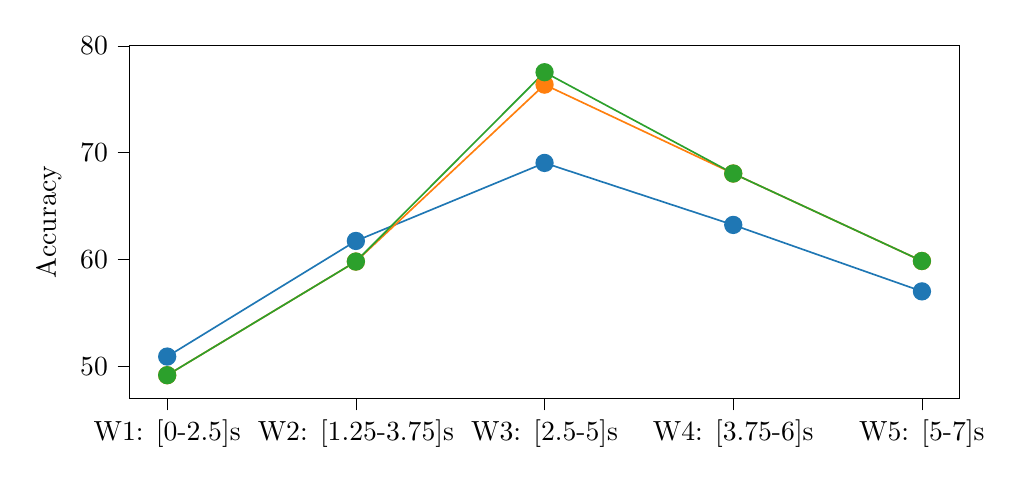
\begin{tikzpicture}

\definecolor{darkgray176}{RGB}{176,176,176}
\definecolor{darkorange25512714}{RGB}{255,127,14}
\definecolor{forestgreen4416044}{RGB}{44,160,44}
\definecolor{steelblue31119180}{RGB}{31,119,180}

\begin{axis}[
tick align=outside,
tick pos=left,
width=\textwidth,
height=0.5\textwidth,
x grid style={darkgray176},
xmin=-0.2, xmax=4.2,
xtick style={color=black},
xtick={0,1,2,3,4},
xticklabels={W1: [0-2.5]s,W2: [1.25-3.75]s,W3: [2.5-5]s,W4: [3.75-6]s,W5: [5-7]s},
y grid style={darkgray176},
ylabel={Accuracy},
ymin=47, ymax=80,
ytick style={color=black}
]
\addplot [semithick, steelblue31119180, mark=*, mark size=3, mark options={solid}]
table {%
0 50.9343747143037
1 61.7496471455741
2 69.0458206616888
3 63.2484703143283
4 57.0335169465879
};
\addplot [semithick, darkorange25512714, mark=*, mark size=3, mark options={solid}]
table {%
0 49.1931422217751
1 59.8215643889214
2 76.3688821731479
3 68.0560775205583
4 59.8733358252709
};
\addplot [semithick, forestgreen4416044, mark=*, mark size=3, mark options={solid}]
table {%
0 49.1931422217751
1 59.8215643889214
2 77.5303862995242
3 68.0560775205583
4 59.8733358252709
};
\end{axis}

\end{tikzpicture}
}
\end{frame}

\begin{frame}{Model level analysis II} 
    \centering
    \resizebox{0.7\linewidth}{!}{% This file was created with tikzplotlib v0.10.1.
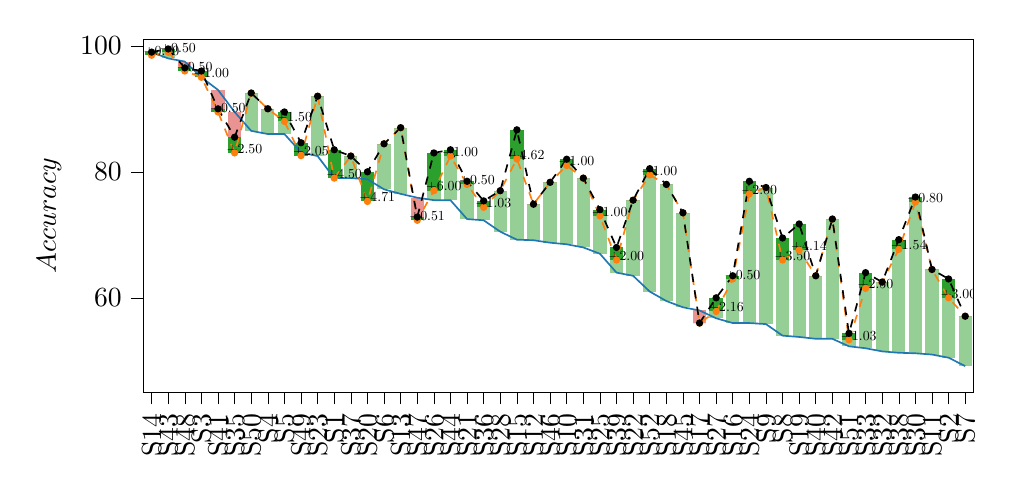
\begin{tikzpicture}

\definecolor{crimson2143940}{RGB}{214,39,40}
\definecolor{darkgray176}{RGB}{176,176,176}
\definecolor{darkorange25512714}{RGB}{255,127,14}
\definecolor{forestgreen4416044}{RGB}{44,160,44}
\definecolor{steelblue31119180}{RGB}{31,119,180}

\begin{axis}[
tick align=outside,
tick pos=left,
width=1\textwidth,
height=.5\textwidth,
x grid style={darkgray176},
xmin=-0.5, xmax=49.5,
xtick style={color=black},
xtick={0,1,2,3,4,5,6,7,8,9,10,11,12,13,14,15,16,17,18,19,20,21,22,23,24,25,26,27,28,29,30,31,32,33,34,35,36,37,38,39,40,41,42,43,44,45,46,47,48,49},
xticklabel style={rotate=90.0,anchor=east},
xticklabels={
  S14,
  S43,
  S48,
  S3,
  S41,
  S35,
  S50,
  S4,
  S5,
  S49,
  S23,
  S1,
  S37,
  S20,
  S6,
  S13,
  S47,
  S26,
  S44,
  S21,
  S36,
  S28,
  S15,
  S12,
  S46,
  S10,
  S31,
  S25,
  S39,
  S22,
  S52,
  S18,
  S45,
  S17,
  S27,
  S16,
  S24,
  S9,
  S8,
  S19,
  S40,
  S42,
  S51,
  S33,
  S32,
  S38,
  S30,
  S11,
  S2,
  S7,
},
y grid style={darkgray176},
ylabel={$Accuracy$},
ymin=45, ymax=101,
ytick style={color=black}
]
\draw[draw=none,fill=crimson2143940,fill opacity=0.5] (axis cs:-0.4,99) rectangle (axis cs:0.4,98.5);
\draw[draw=none,fill=forestgreen4416044,fill opacity=0.5] (axis cs:0.6,98) rectangle (axis cs:1.4,99);
\draw[draw=none,fill=crimson2143940,fill opacity=0.5] (axis cs:1.6,97.5) rectangle (axis cs:2.4,96);
\draw[draw=none,fill=crimson2143940,fill opacity=0.5] (axis cs:2.6,95) rectangle (axis cs:3.4,95);
\draw[draw=none,fill=crimson2143940,fill opacity=0.5] (axis cs:3.6,93) rectangle (axis cs:4.4,89.5);
\draw[draw=none,fill=crimson2143940,fill opacity=0.5] (axis cs:4.6,89.5) rectangle (axis cs:5.4,83);
\draw[draw=none,fill=forestgreen4416044,fill opacity=0.5] (axis cs:5.6,86.5) rectangle (axis cs:6.4,92.5);
\draw[draw=none,fill=forestgreen4416044,fill opacity=0.5] (axis cs:6.6,86) rectangle (axis cs:7.4,90);
\draw[draw=none,fill=forestgreen4416044,fill opacity=0.5] (axis cs:7.6,86) rectangle (axis cs:8.4,88);
\draw[draw=none,fill=crimson2143940,fill opacity=0.5] (axis cs:8.6,83.0769230769231) rectangle (axis cs:9.4,82.5641025641026);
\draw[draw=none,fill=forestgreen4416044,fill opacity=0.5] (axis cs:9.6,82.5) rectangle (axis cs:10.4,92);
\draw[draw=none,fill=crimson2143940,fill opacity=0.5] (axis cs:10.6,79) rectangle (axis cs:11.4,79);
\draw[draw=none,fill=forestgreen4416044,fill opacity=0.5] (axis cs:11.6,79) rectangle (axis cs:12.4,82.5);
\draw[draw=none,fill=crimson2143940,fill opacity=0.5] (axis cs:12.6,78.8235294117647) rectangle (axis cs:13.4,75.2941176470588);
\draw[draw=none,fill=forestgreen4416044,fill opacity=0.5] (axis cs:13.6,77.2222222222222) rectangle (axis cs:14.4,84.4444444444444);
\draw[draw=none,fill=forestgreen4416044,fill opacity=0.5] (axis cs:14.6,76.5) rectangle (axis cs:15.4,87);
\draw[draw=none,fill=crimson2143940,fill opacity=0.5] (axis cs:15.6,75.8974358974359) rectangle (axis cs:16.4,72.3076923076923);
\draw[draw=none,fill=forestgreen4416044,fill opacity=0.5] (axis cs:16.6,75.5) rectangle (axis cs:17.4,77);
\draw[draw=none,fill=forestgreen4416044,fill opacity=0.5] (axis cs:17.6,75.5) rectangle (axis cs:18.4,82.5);
\draw[draw=none,fill=forestgreen4416044,fill opacity=0.5] (axis cs:18.6,72.5) rectangle (axis cs:19.4,78);
\draw[draw=none,fill=forestgreen4416044,fill opacity=0.5] (axis cs:19.6,72.3076923076923) rectangle (axis cs:20.4,74.3589743589744);
\draw[draw=none,fill=forestgreen4416044,fill opacity=0.5] (axis cs:20.6,70.5) rectangle (axis cs:21.4,77);
\draw[draw=none,fill=forestgreen4416044,fill opacity=0.5] (axis cs:21.6,69.2307692307692) rectangle (axis cs:22.4,82.051282051282);
\draw[draw=none,fill=forestgreen4416044,fill opacity=0.5] (axis cs:22.6,69.1428571428572) rectangle (axis cs:23.4,74.8571428571429);
\draw[draw=none,fill=forestgreen4416044,fill opacity=0.5] (axis cs:23.6,68.75) rectangle (axis cs:24.4,78.3333333333333);
\draw[draw=none,fill=forestgreen4416044,fill opacity=0.5] (axis cs:24.6,68.5) rectangle (axis cs:25.4,81);
\draw[draw=none,fill=forestgreen4416044,fill opacity=0.5] (axis cs:25.6,68) rectangle (axis cs:26.4,79);
\draw[draw=none,fill=forestgreen4416044,fill opacity=0.5] (axis cs:26.6,67) rectangle (axis cs:27.4,73);
\draw[draw=none,fill=forestgreen4416044,fill opacity=0.5] (axis cs:27.6,64) rectangle (axis cs:28.4,66);
\draw[draw=none,fill=forestgreen4416044,fill opacity=0.5] (axis cs:28.6,63.5) rectangle (axis cs:29.4,75.5);
\draw[draw=none,fill=forestgreen4416044,fill opacity=0.5] (axis cs:29.6,61) rectangle (axis cs:30.4,79.5);
\draw[draw=none,fill=forestgreen4416044,fill opacity=0.5] (axis cs:30.6,59.5) rectangle (axis cs:31.4,78);
\draw[draw=none,fill=forestgreen4416044,fill opacity=0.5] (axis cs:31.6,58.5) rectangle (axis cs:32.4,73.5);
\draw[draw=none,fill=crimson2143940,fill opacity=0.5] (axis cs:32.6,58) rectangle (axis cs:33.4,56);
\draw[draw=none,fill=forestgreen4416044,fill opacity=0.5] (axis cs:33.6,56.7567567567568) rectangle (axis cs:34.4,57.8378378378379);
\draw[draw=none,fill=forestgreen4416044,fill opacity=0.5] (axis cs:34.6,56) rectangle (axis cs:35.4,63);
\draw[draw=none,fill=forestgreen4416044,fill opacity=0.5] (axis cs:35.6,56) rectangle (axis cs:36.4,76.5);
\draw[draw=none,fill=forestgreen4416044,fill opacity=0.5] (axis cs:36.6,55.8333333333333) rectangle (axis cs:37.4,77.5);
\draw[draw=none,fill=forestgreen4416044,fill opacity=0.5] (axis cs:37.6,54) rectangle (axis cs:38.4,66);
\draw[draw=none,fill=forestgreen4416044,fill opacity=0.5] (axis cs:38.6,53.7931034482759) rectangle (axis cs:39.4,67.5862068965517);
\draw[draw=none,fill=forestgreen4416044,fill opacity=0.5] (axis cs:39.6,53.5) rectangle (axis cs:40.4,63.5);
\draw[draw=none,fill=forestgreen4416044,fill opacity=0.5] (axis cs:40.6,53.5) rectangle (axis cs:41.4,72.5);
\draw[draw=none,fill=forestgreen4416044,fill opacity=0.5] (axis cs:41.6,52.3076923076923) rectangle (axis cs:42.4,53.3333333333333);
\draw[draw=none,fill=forestgreen4416044,fill opacity=0.5] (axis cs:42.6,52) rectangle (axis cs:43.4,61.5);
\draw[draw=none,fill=forestgreen4416044,fill opacity=0.5] (axis cs:43.6,51.5) rectangle (axis cs:44.4,62.5);
\draw[draw=none,fill=forestgreen4416044,fill opacity=0.5] (axis cs:44.6,51.2820512820513) rectangle (axis cs:45.4,67.6923076923077);
\draw[draw=none,fill=forestgreen4416044,fill opacity=0.5] (axis cs:45.6,51.2) rectangle (axis cs:46.4,75.2);
\draw[draw=none,fill=forestgreen4416044,fill opacity=0.5] (axis cs:46.6,51) rectangle (axis cs:47.4,64.5);
\draw[draw=none,fill=forestgreen4416044,fill opacity=0.5] (axis cs:47.6,50.5) rectangle (axis cs:48.4,60);
\draw[draw=none,fill=forestgreen4416044,fill opacity=0.5] (axis cs:48.6,49.1666666666667) rectangle (axis cs:49.4,57.0833333333333);
\draw[draw=none,fill=forestgreen4416044] (axis cs:-0.4,98.5) rectangle (axis cs:0.4,99);
\draw[draw=none,fill=forestgreen4416044] (axis cs:0.6,99) rectangle (axis cs:1.4,99.5);
\draw[draw=none,fill=forestgreen4416044] (axis cs:1.6,96) rectangle (axis cs:2.4,96.5);
\draw[draw=none,fill=forestgreen4416044] (axis cs:2.6,95) rectangle (axis cs:3.4,96);
\draw[draw=none,fill=forestgreen4416044] (axis cs:3.6,89.5) rectangle (axis cs:4.4,90);
\draw[draw=none,fill=forestgreen4416044] (axis cs:4.6,83) rectangle (axis cs:5.4,85.5);
\draw[draw=none,fill=crimson2143940] (axis cs:5.6,92.5) rectangle (axis cs:6.4,92.5);
\draw[draw=none,fill=crimson2143940] (axis cs:6.6,90) rectangle (axis cs:7.4,90);
\draw[draw=none,fill=forestgreen4416044] (axis cs:7.6,88) rectangle (axis cs:8.4,89.5);
\draw[draw=none,fill=forestgreen4416044] (axis cs:8.6,82.5641025641026) rectangle (axis cs:9.4,84.6153846153846);
\draw[draw=none,fill=crimson2143940] (axis cs:9.6,92) rectangle (axis cs:10.4,92);
\draw[draw=none,fill=forestgreen4416044] (axis cs:10.6,79) rectangle (axis cs:11.4,83.5);
\draw[draw=none,fill=crimson2143940] (axis cs:11.6,82.5) rectangle (axis cs:12.4,82.5);
\draw[draw=none,fill=forestgreen4416044] (axis cs:12.6,75.2941176470588) rectangle (axis cs:13.4,80);
\draw[draw=none,fill=crimson2143940] (axis cs:13.6,84.4444444444444) rectangle (axis cs:14.4,84.4444444444444);
\draw[draw=none,fill=crimson2143940] (axis cs:14.6,87) rectangle (axis cs:15.4,87);
\draw[draw=none,fill=forestgreen4416044] (axis cs:15.6,72.3076923076923) rectangle (axis cs:16.4,72.8205128205128);
\draw[draw=none,fill=forestgreen4416044] (axis cs:16.6,77) rectangle (axis cs:17.4,83);
\draw[draw=none,fill=forestgreen4416044] (axis cs:17.6,82.5) rectangle (axis cs:18.4,83.5);
\draw[draw=none,fill=forestgreen4416044] (axis cs:18.6,78) rectangle (axis cs:19.4,78.5);
\draw[draw=none,fill=forestgreen4416044] (axis cs:19.6,74.3589743589744) rectangle (axis cs:20.4,75.3846153846154);
\draw[draw=none,fill=crimson2143940] (axis cs:20.6,77) rectangle (axis cs:21.4,77);
\draw[draw=none,fill=forestgreen4416044] (axis cs:21.6,82.051282051282) rectangle (axis cs:22.4,86.6666666666667);
\draw[draw=none,fill=crimson2143940] (axis cs:22.6,74.8571428571429) rectangle (axis cs:23.4,74.8571428571429);
\draw[draw=none,fill=crimson2143940] (axis cs:23.6,78.3333333333333) rectangle (axis cs:24.4,78.3333333333333);
\draw[draw=none,fill=forestgreen4416044] (axis cs:24.6,81) rectangle (axis cs:25.4,82);
\draw[draw=none,fill=crimson2143940] (axis cs:25.6,79) rectangle (axis cs:26.4,79);
\draw[draw=none,fill=forestgreen4416044] (axis cs:26.6,73) rectangle (axis cs:27.4,74);
\draw[draw=none,fill=forestgreen4416044] (axis cs:27.6,66) rectangle (axis cs:28.4,68);
\draw[draw=none,fill=crimson2143940] (axis cs:28.6,75.5) rectangle (axis cs:29.4,75.5);
\draw[draw=none,fill=forestgreen4416044] (axis cs:29.6,79.5) rectangle (axis cs:30.4,80.5);
\draw[draw=none,fill=crimson2143940] (axis cs:30.6,78) rectangle (axis cs:31.4,78);
\draw[draw=none,fill=crimson2143940] (axis cs:31.6,73.5) rectangle (axis cs:32.4,73.5);
\draw[draw=none,fill=crimson2143940] (axis cs:32.6,56) rectangle (axis cs:33.4,56);
\draw[draw=none,fill=forestgreen4416044] (axis cs:33.6,57.8378378378378) rectangle (axis cs:34.4,60);
\draw[draw=none,fill=forestgreen4416044] (axis cs:34.6,63) rectangle (axis cs:35.4,63.5);
\draw[draw=none,fill=forestgreen4416044] (axis cs:35.6,76.5) rectangle (axis cs:36.4,78.5);
\draw[draw=none,fill=crimson2143940] (axis cs:36.6,77.5) rectangle (axis cs:37.4,77.5);
\draw[draw=none,fill=forestgreen4416044] (axis cs:37.6,66) rectangle (axis cs:38.4,69.5);
\draw[draw=none,fill=forestgreen4416044] (axis cs:38.6,67.5862068965517) rectangle (axis cs:39.4,71.7241379310345);
\draw[draw=none,fill=crimson2143940] (axis cs:39.6,63.5) rectangle (axis cs:40.4,63.5);
\draw[draw=none,fill=forestgreen4416044] (axis cs:40.6,72.5) rectangle (axis cs:41.4,72.5);
\draw[draw=none,fill=forestgreen4416044] (axis cs:41.6,53.3333333333333) rectangle (axis cs:42.4,54.3589743589744);
\draw[draw=none,fill=forestgreen4416044] (axis cs:42.6,61.5) rectangle (axis cs:43.4,64);
\draw[draw=none,fill=crimson2143940] (axis cs:43.6,62.5) rectangle (axis cs:44.4,62.5);
\draw[draw=none,fill=forestgreen4416044] (axis cs:44.6,67.6923076923077) rectangle (axis cs:45.4,69.2307692307692);
\draw[draw=none,fill=forestgreen4416044] (axis cs:45.6,75.2) rectangle (axis cs:46.4,76);
\draw[draw=none,fill=crimson2143940] (axis cs:46.6,64.5) rectangle (axis cs:47.4,64.5);
\draw[draw=none,fill=forestgreen4416044] (axis cs:47.6,60) rectangle (axis cs:48.4,63);
\draw[draw=none,fill=crimson2143940] (axis cs:48.6,57.0833333333333) rectangle (axis cs:49.4,57.0833333333333);
\addplot [semithick, steelblue31119180]
table {%
0 99
1 98
2 97.5
3 95
4 93
5 89.5
6 86.5
7 86
8 86
9 83.0769230769231
10 82.5
11 79
12 79
13 78.8235294117647
14 77.2222222222222
15 76.5
16 75.8974358974359
17 75.5
18 75.5
19 72.5
20 72.3076923076923
21 70.5
22 69.2307692307692
23 69.1428571428572
24 68.75
25 68.5
26 68
27 67
28 64
29 63.5
30 61
31 59.5
32 58.5
33 58
34 56.7567567567568
35 56
36 56
37 55.8333333333333
38 54
39 53.7931034482759
40 53.5
41 53.5
42 52.3076923076923
43 52
44 51.5
45 51.2820512820513
46 51.2
47 51
48 50.5
49 49.1666666666667
};
\addplot [semithick, darkorange25512714, mark=*, mark size=1, mark options={solid}, dashed]
table {%
0 98.5
1 99
2 96
3 95
4 89.5
5 83
6 92.5
7 90
8 88
9 82.5641025641026
10 92
11 79
12 82.5
13 75.2941176470588
14 84.4444444444444
15 87
16 72.3076923076923
17 77
18 82.5
19 78
20 74.3589743589744
21 77
22 82.051282051282
23 74.8571428571429
24 78.3333333333333
25 81
26 79
27 73
28 66
29 75.5
30 79.5
31 78
32 73.5
33 56
34 57.8378378378378
35 63
36 76.5
37 77.5
38 66
39 67.5862068965517
40 63.5
41 72.5
42 53.3333333333333
43 61.5
44 62.5
45 67.6923076923077
46 75.2
47 64.5
48 60
49 57.0833333333333
};
\addplot [semithick, black, mark=*, mark size=1, mark options={solid}, dashed]
table {%
0 99
1 99.5
2 96.5
3 96
4 90
5 85.5
6 92.5
7 90
8 89.5
9 84.6153846153846
10 92
11 83.5
12 82.5
13 80
14 84.4444444444444
15 87
16 72.8205128205128
17 83
18 83.5
19 78.5
20 75.3846153846154
21 77
22 86.6666666666667
23 74.8571428571429
24 78.3333333333333
25 82
26 79
27 74
28 68
29 75.5
30 80.5
31 78
32 73.5
33 56
34 60
35 63.5
36 78.5
37 77.5
38 69.5
39 71.7241379310345
40 63.5
41 72.5
42 54.3589743589744
43 64
44 62.5
45 69.2307692307692
46 76
47 64.5
48 63
49 57.0833333333333
};
\draw (axis cs:0.6,97.5) node[
  scale=0.5,
  anchor=south,
  text=black,
  rotate=0.0
]{+0.50};
\draw (axis cs:1.6,98) node[
  scale=0.5,
  anchor=south,
  text=black,
  rotate=0.0
]{+0.50};
\draw (axis cs:2.6,95) node[
  scale=0.5,
  anchor=south,
  text=black,
  rotate=0.0
]{+0.50};
\draw (axis cs:3.6,94) node[
  scale=0.5,
  anchor=south,
  text=black,
  rotate=0.0
]{+1.00};
\draw (axis cs:4.6,88.5) node[
  scale=0.5,
  anchor=south,
  text=black,
  rotate=0.0
]{+0.50};
\draw (axis cs:5.6,82) node[
  scale=0.5,
  anchor=south,
  text=black,
  rotate=0.0
]{+2.50};
\draw (axis cs:8.6,87) node[
  scale=0.5,
  anchor=south,
  text=black,
  rotate=0.0
]{+1.50};
\draw (axis cs:9.6,81.5641025641026) node[
  scale=0.5,
  anchor=south,
  text=black,
  rotate=0.0
]{+2.05};
\draw (axis cs:11.6,78) node[
  scale=0.5,
  anchor=south,
  text=black,
  rotate=0.0
]{+4.50};
\draw (axis cs:13.6,74.2941176470588) node[
  scale=0.5,
  anchor=south,
  text=black,
  rotate=0.0
]{+4.71};
\draw (axis cs:16.6,71.3076923076923) node[
  scale=0.5,
  anchor=south,
  text=black,
  rotate=0.0
]{+0.51};
\draw (axis cs:17.6,76) node[
  scale=0.5,
  anchor=south,
  text=black,
  rotate=0.0
]{+6.00};
\draw (axis cs:18.6,81.5) node[
  scale=0.5,
  anchor=south,
  text=black,
  rotate=0.0
]{+1.00};
\draw (axis cs:19.6,77) node[
  scale=0.5,
  anchor=south,
  text=black,
  rotate=0.0
]{+0.50};
\draw (axis cs:20.6,73.3589743589744) node[
  scale=0.5,
  anchor=south,
  text=black,
  rotate=0.0
]{+1.03};
\draw (axis cs:22.6,81.051282051282) node[
  scale=0.5,
  anchor=south,
  text=black,
  rotate=0.0
]{+4.62};
\draw (axis cs:25.6,80) node[
  scale=0.5,
  anchor=south,
  text=black,
  rotate=0.0
]{+1.00};
\draw (axis cs:27.6,72) node[
  scale=0.5,
  anchor=south,
  text=black,
  rotate=0.0
]{+1.00};
\draw (axis cs:28.6,65) node[
  scale=0.5,
  anchor=south,
  text=black,
  rotate=0.0
]{+2.00};
\draw (axis cs:30.6,78.5) node[
  scale=0.5,
  anchor=south,
  text=black,
  rotate=0.0
]{+1.00};
\draw (axis cs:34.6,56.8378378378378) node[
  scale=0.5,
  anchor=south,
  text=black,
  rotate=0.0
]{+2.16};
\draw (axis cs:35.6,62) node[
  scale=0.5,
  anchor=south,
  text=black,
  rotate=0.0
]{+0.50};
\draw (axis cs:36.6,75.5) node[
  scale=0.5,
  anchor=south,
  text=black,
  rotate=0.0
]{+2.00};
\draw (axis cs:38.6,65) node[
  scale=0.5,
  anchor=south,
  text=black,
  rotate=0.0
]{+3.50};
\draw (axis cs:39.6,66.5862068965517) node[
  scale=0.5,
  anchor=south,
  text=black,
  rotate=0.0
]{+4.14};
\draw (axis cs:42.6,52.3333333333333) node[
  scale=0.5,
  anchor=south,
  text=black,
  rotate=0.0
]{+1.03};
\draw (axis cs:43.6,60.5) node[
  scale=0.5,
  anchor=south,
  text=black,
  rotate=0.0
]{+2.50};
\draw (axis cs:45.6,66.6923076923077) node[
  scale=0.5,
  anchor=south,
  text=black,
  rotate=0.0
]{+1.54};
\draw (axis cs:46.6,74.2) node[
  scale=0.5,
  anchor=south,
  text=black,
  rotate=0.0
]{+0.80};
\draw (axis cs:48.6,59) node[
  scale=0.5,
  anchor=south,
  text=black,
  rotate=0.0
]{+3.00};
\end{axis}

\end{tikzpicture}}
\end{frame}

\begin{frame}{Group level analysis I}
    \centering
    \resizebox{0.7\linewidth}{!}{\input{figures/semaforo_3.tex}}
\end{frame}

\begin{frame}{Group level analysis II}
    \begin{table}
        \centering
        \begin{tabular}{|c|c|c|c|}
            \hline
            Strategy & G I & G II  & G III \\
            \hline
            EEGnet & 90.55 $\pm$ 5.88 & 72.15 $\pm$ 4.87 & 54.27 $\pm$ 3.21 \\
            KCS-FCnet & 91.46 $\pm$ 5.31   &  77.85 $\pm$ 4.76 & 66.66 $\pm$ 7.88 \\
            IRKCS-FCnet & \textbf{92.28 $\pm$ 4.79}  & \textbf{79.26 $\pm$ 4.93}  & \textbf{67.77$\pm$ 7.83} \\
            \hline
        \end{tabular}
    \end{table}
\end{frame}

\begin{frame}{Group level analysis III}
  \centering
  \resizebox{0.7\linewidth}{!}{% This file was created with tikzplotlib v0.10.1.
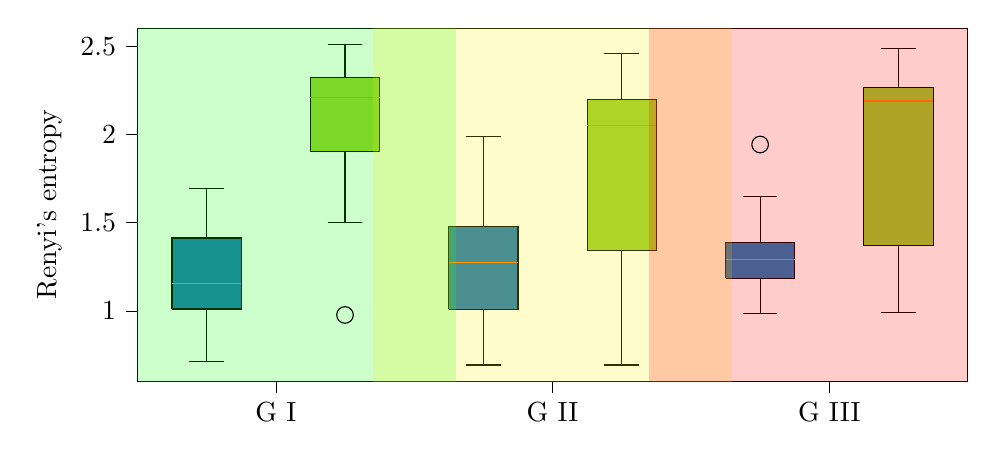
\begin{tikzpicture}

\definecolor{darkgray176}{RGB}{176,176,176}
\definecolor{darkorange25512714}{RGB}{255,127,14}

\definecolor{steelblue31119180}{RGB}{31,119,180}
\definecolor{yellowgreen}{RGB}{154, 205, 50}

\begin{axis}[
tick align=outside,
tick pos=left,
x grid style={darkgray176},
xmin=0.5, xmax=6.5,
width=\textwidth,
height=0.5\textwidth,
xtick style={color=black},
xtick={1.5,3.5,5.5},
xticklabels={G I,G II,G III},
y grid style={darkgray176},
ylabel={Renyi's entropy},
ymin=0.602331051230431, ymax=2.60267644226551,
ytick style={color=black}
]
\addplot [black, fill=steelblue31119180]
table {%
0.75 1.0111822783947
1.25 1.0111822783947
1.25 1.41367989778519
0.75 1.41367989778519
0.75 1.0111822783947
};
\addplot [black]
table {%
1 1.0111822783947
1 0.714407742023468
};
\addplot [black]
table {%
1 1.41367989778519
1 1.69561421871185
};
\addplot [black]
table {%
0.875 0.714407742023468
1.125 0.714407742023468
};
\addplot [black]
table {%
0.875 1.69561421871185
1.125 1.69561421871185
};
\addplot [black, fill=yellowgreen]
table {%
1.75 1.90198284387589
2.25 1.90198284387589
2.25 2.32088589668274
1.75 2.32088589668274
1.75 1.90198284387589
};
\addplot [black]
table {%
2 1.90198284387589
2 1.49933624267578
};
\addplot [black]
table {%
2 2.32088589668274
2 2.51175165176392
};
\addplot [black]
table {%
1.875 1.49933624267578
2.125 1.49933624267578
};
\addplot [black]
table {%
1.875 2.51175165176392
2.125 2.51175165176392
};
\addplot [black, mark=o, mark size=3, mark options={solid,fill opacity=0}, only marks]
table {%
2 0.977205276489258
};
\addplot [black, fill=steelblue31119180]
table {%
2.75 1.00999590754509
3.25 1.00999590754509
3.25 1.47894328832626
2.75 1.47894328832626
2.75 1.00999590754509
};
\addplot [black]
table {%
3 1.00999590754509
3 0.693255841732025
};
\addplot [black]
table {%
3 1.47894328832626
3 1.99005436897278
};
\addplot [black]
table {%
2.875 0.693255841732025
3.125 0.693255841732025
};
\addplot [black]
table {%
2.875 1.99005436897278
3.125 1.99005436897278
};
\addplot [black, fill=yellowgreen]
table {%
3.75 1.34344190359116
4.25 1.34344190359116
4.25 2.19900119304657
3.75 2.19900119304657
3.75 1.34344190359116
};
\addplot [black]
table {%
4 1.34344190359116
4 0.69325590133667
};
\addplot [black]
table {%
4 2.19900119304657
4 2.46135926246643
};
\addplot [black]
table {%
3.875 0.69325590133667
4.125 0.69325590133667
};
\addplot [black]
table {%
3.875 2.46135926246643
4.125 2.46135926246643
};
\addplot [black, fill=steelblue31119180]
table {%
4.75 1.18452069163322
5.25 1.18452069163322
5.25 1.38582560420036
4.75 1.38582560420036
4.75 1.18452069163322
};
\addplot [black]
table {%
5 1.18452069163322
5 0.987190246582031
};
\addplot [black]
table {%
5 1.38582560420036
5 1.65000188350677
};
\addplot [black]
table {%
4.875 0.987190246582031
5.125 0.987190246582031
};
\addplot [black]
table {%
4.875 1.65000188350677
5.125 1.65000188350677
};
\addplot [black, mark=o, mark size=3, mark options={solid,fill opacity=0}, only marks]
table {%
5 1.94329965114594
};
\addplot [black, fill=yellowgreen]
table {%
5.75 1.36978048086166
6.25 1.36978048086166
6.25 2.2656888961792
5.75 2.2656888961792
5.75 1.36978048086166
};
\addplot [black]
table {%
6 1.36978048086166
6 0.992337465286255
};
\addplot [black]
table {%
6 2.2656888961792
6 2.48897361755371
};
\addplot [black]
table {%
5.875 0.992337465286255
6.125 0.992337465286255
};
\addplot [black]
table {%
5.875 2.48897361755371
6.125 2.48897361755371
};
\addplot [darkorange25512714]
table {%
0.75 1.15490031242371
1.25 1.15490031242371
};
\addplot [darkorange25512714]
table {%
1.75 2.20872807502747
2.25 2.20872807502747
};
\addplot [darkorange25512714]
table {%
2.75 1.27640020847321
3.25 1.27640020847321
};
\addplot [darkorange25512714]
table {%
3.75 2.0507481098175
4.25 2.0507481098175
};
\addplot [darkorange25512714]
table {%
4.75 1.29070019721985
5.25 1.29070019721985
};
\addplot [darkorange25512714]
table {%
5.75 2.19007635116577
6.25 2.19007635116577
};
\path [draw=green, opacity=0.2, line width=130pt]
(axis cs:1.5,0.1)
--(axis cs:1.5,3);

\path [draw=yellow, opacity=0.2, line width=130pt]
(axis cs:3.5,0.1)
--(axis cs:3.5,3);

\path [draw=red, opacity=0.2, line width=130pt]
(axis cs:5.5,0.1)
--(axis cs:5.5,3);
\end{axis}

\end{tikzpicture}
}
\end{frame}

\begin{frame}{Post-hoc interpretability}
    \begin{table}[h!]
        \centering
        \begin{tabular}{|c|c|c|}
        \hline
        \textbf{Group} & \textbf{KCS-FCnet vs. Random} & \textbf{RKCS-FCnet vs. Random} \\ \hline
        \textbf{G I} & 0.00077* & 0.00230* \\
        \textbf{G II} & 0.00368* & 0.00434* \\
        \textbf{G III} & 0.00108* & 0.00074* \\ \hline
        \end{tabular}
        \end{table}

        \begin{table}[h!]
            \centering
            \begin{tabular}{|l|l|c|c|c|c|c|}
            \hline
            \textbf{Strategy} & \textbf{Group} & \textbf{25\%} & \textbf{20\%} & \textbf{15\%} & \textbf{10\%} & \textbf{5\%} \\ \hline
            \multirow{3}{*}{\textbf{KCS-FCnet}} & \textbf{G I} & 40.51 & 37.93 & 35.97 & 30.25 & 17.12 \\
             & \textbf{G II} & 40.10 & 39.00 & 36.46 & \cellcolor{GII!80}28.60 & 17.72 \\
             & \textbf{G III} & 39.05 & 36.98 & 31.99 & 25.28 & 15.02 \\ \hline
            \multirow{3}{*}{\textbf{RKCS-FCnet}} & \textbf{G I} &  44.80 & 39.21 &  37.79 &  30.55 & \cellcolor{GI!80} 22.46 \\
             & \textbf{G II} & 41.08 & 40.01 & 36.77 & 27.28 & 18.84 \\
             & \textbf{G III} & 39.65 & 37.30 & 33.12 & \cellcolor{GIII!70}27.10 & 16.80 \\ \hline
            \end{tabular}
            \end{table}
\end{frame}

\begin{frame}{Intrinsic interpretability I}
    \def \kerrwidth {0.3\linewidth}
\def \kerrg {0.3\linewidth}
\begin{figure}[h!]
\centering
\scalebox{0.7}[0.7]{
\begin{tabular}{ccc}
\centering
\textbf{G I} & \textbf{G II} & \textbf{G III} \\
{\resizebox{\kerrwidth}{!}{\includegraphics[trim=80 10 80 10, clip]{../Tesis_document/Figures/Objective_3/group_G I_top10_channels.pdf}}} & 
{\resizebox{\kerrwidth}{!}{\includegraphics[trim=80 10 80 10, clip]{../Tesis_document/Figures/Objective_3/group_G II_top10_channels.pdf}}} & {\resizebox{\kerrwidth}{!}{\includegraphics[trim=80 10 80 10, clip]{../Tesis_document/Figures/Objective_3/group_G III_top10_channels.pdf}}} \\
\end{tabular}
}
\end{figure}
\end{frame}


\begin{frame}{Intrinsic interpretability II}
    \def \kerrwidth {0.63\linewidth}
    \centering
    \scalebox{0.7}{
        \begin{tabular}{cc}
            \rotatebox{90}{\hspace{12mm} \textbf{G I}} &
            \resizebox{\kerrwidth}{!}{\includegraphics[trim=25 115 35 120, clip]{../Tesis_document/Figures/Objective_3/group_G I_top10_channels_PSD.pdf}} \\
            
            \rotatebox{90}{\hspace{12mm} \textbf{G II}} &
            \resizebox{\kerrwidth}{!}{\includegraphics[trim=25 115 35 120, clip]{../Tesis_document/Figures/Objective_3/group_G II_top10_channels_PSD.pdf}} \\
            
            \rotatebox{90}{\hspace{21mm} \textbf{G III}} &
            \resizebox{\kerrwidth}{!}{\includegraphics[trim=25 80 35 120, clip]{../Tesis_document/Figures/Objective_3/group_G III_top10_channels_PSD.pdf}} \\
        \end{tabular}
    }
\end{frame}


\begin{frame}{Intrinsic interpretability III}
\def \kerrwidth {0.3\linewidth}
\begin{figure}[h!]
\centering
\scalebox{0.5}[0.5]{
\begin{tabular}{ccccc}
\centering
& \textbf{G I} & \textbf{G II} & \textbf{G III} & \\
{\rotatebox{90}{\hspace{15mm} \textbf{Left class}}} & 
{\resizebox{\kerrwidth}{!}{\includegraphics[trim=80 10 80 10, clip]{../Tesis_document/Figures/Objective_3/class_Left_group_G I_GFC_renyi.pdf}}} & 
{\resizebox{\kerrwidth}{!}{\includegraphics[trim=80 10 80 10, clip]{../Tesis_document/Figures/Objective_3/class_Left_group_G II_GFC_renyi.pdf}}} & {\resizebox{\kerrwidth}{!}{\includegraphics[trim=80 10 80 10, clip]{../Tesis_document/Figures/Objective_3/class_Left_group_G III_GFC_renyi.pdf}}} & \\
{\rotatebox{90}{\hspace{15mm} \textbf{Right class}}} & 
{\resizebox{\kerrwidth}{!}{\includegraphics[trim=80 10 80 10, clip]{../Tesis_document/Figures/Objective_3/class_Right_group_G I_GFC_renyi.pdf}}} & 
{\resizebox{\kerrwidth}{!}{\includegraphics[trim=80 10 80 10, clip]{../Tesis_document/Figures/Objective_3/class_Right_group_G II_GFC_renyi.pdf}}} & {\resizebox{\kerrwidth}{!}{\includegraphics[trim=80 10 80 10, clip]{../Tesis_document/Figures/Objective_3/class_Right_group_G III_GFC_renyi.pdf}}} & \\
&\multicolumn{3}{c}{\resizebox{0.69\linewidth}{!}{\includegraphics[trim=0 0 0 250, clip]{../Tesis_document/Figures/Objective_3/colorbar.pdf}}} \\
\end{tabular}
}
\end{figure}

\end{frame}

\begin{frame}{Individual subject analysis I}
\def \kerrwidth {0.95\linewidth}
\begin{figure}[h!]
\centering
\scalebox{0.7}[0.7]{
\begin{tabular}{ccc}
\centering
    &\hspace{10mm} \textbf{Direct label} \hspace{40mm} \textbf{Cross-label} & \\
{\rotatebox{90}{\hspace{10mm} \textbf{Subject 4 - G I}}} &
{\resizebox{\kerrwidth}{!}{\includegraphics{../Tesis_document/Figures/Objective_3/subject_4_group_GI.pdf}}} \\

& {\hspace{20mm}  \resizebox{0.5\linewidth}{!}{\includegraphics[trim=0 0 0 250, clip]{../Tesis_document/Figures/Objective_3/colorbar2.pdf}}} &\\
\end{tabular}
}
\end{figure}
\end{frame}

\begin{frame}{Individual subject analysis II}
    \def \kerrwidth {0.95\linewidth}
    \begin{figure}[h!]
    \centering
    \scalebox{0.7}[0.7]{
    \begin{tabular}{ccc}
    \centering
        &\hspace{10mm} \textbf{Direct label} \hspace{40mm} \textbf{Cross-label} & \\   
    {\rotatebox{90}{\hspace{10mm} \textbf{Subject 42 - G II}}} &
    {\resizebox{\kerrwidth}{!}{\includegraphics{../Tesis_document/Figures/Objective_3/subject_42_group_GII.pdf}}} \\
        & {\hspace{20mm}  \resizebox{0.5\linewidth}{!}{\includegraphics[trim=0 0 0 250, clip]{../Tesis_document/Figures/Objective_3/colorbar2.pdf}}} &\\
    \end{tabular}
    }
    \end{figure}
\end{frame}

\begin{frame}{Individual subject analysis III}
    \def \kerrwidth {0.95\linewidth}
    \begin{figure}[h!]
    \centering
    \scalebox{0.7}[0.7]{
    \begin{tabular}{ccc}
    \centering
        &\hspace{10mm} \textbf{Direct label} \hspace{40mm} \textbf{Cross-label} & \\   
    {\rotatebox{90}{\hspace{10mm} \textbf{Subject 51 - G III}}} &
    {\resizebox{\kerrwidth}{!}{\includegraphics[trim=0 10 0 0, clip]{../Tesis_document/Figures/Objective_3/subject_51_group_GIII.pdf}}} \\
        & {\hspace{20mm}  \resizebox{0.5\linewidth}{!}{\includegraphics[trim=0 0 0 250, clip]{../Tesis_document/Figures/Objective_3/colorbar2.pdf}}} &\\
    \end{tabular}
    }
    \end{figure}
\end{frame}


\section{Conclusions}
\begin{frame}{Conclusions}
    \begin{itemize}
        \item conclusions
    \end{itemize}
\end{frame}


\section{Future work}
\begin{frame}{Future work}
    \begin{itemize}
        \item Future work
    \end{itemize}
\end{frame}

\section{References}
% ------------------------------------------------------------------------
\begin{frame}[allowframebreaks]%,noframenumbering]
\frametitle{References}
{\tiny 
\bibliographystyle{apalike}
\bibliography{../Tesis_document/References}
}
\end{frame}

\end{document}